%  Copyright (C) 2018-2021 by the authors of the World Builder code.
%
%  This file is part of the World Builder.
%
%   This program is free software: you can redistribute it and/or modify
%   it under the terms of the GNU Lesser General Public License as published
%   by the Free Software Foundation, either version 2 of the License, or
%   (at your option) any later version.
%
%   This program is distributed in the hope that it will be useful,
%   but WITHOUT ANY WARRANTY; without even the implied warranty of
%   MERCHANTABILITY or FITNESS FOR A PARTICULAR PURPOSE.  See the
%   GNU Lesser General Public License for more details.
%
%   You should have received a copy of the GNU Lesser General Public License
%   along with this program.  If not, see <https://www.gnu.org/licenses/>.

\documentclass{book} 

\usepackage[utf8]{inputenc}
\usepackage{graphicx}
\usepackage{tikz}
\usepackage{fancyhdr}
\usepackage{titletoc} %needed for chaning the table of contents
%\usepackage{calc}

\usepackage{enumitem}
\setlistdepth{9}
%\setlist{labelindent=1.5em}
%\setlist{leftmargin=0.0em}
%\setlength{\itemindent}{-2em}
\setlist[enumerate,1]{label*=\arabic*., leftmargin=*}%, itemindent=-0em}
\setlist[enumerate,2]{label*=\arabic*., leftmargin=*}%, itemindent=-0.25em}%=(\Roman*)}
\setlist[enumerate,3]{label*=\arabic*., leftmargin=*}%, itemindent=-0.5em}%=(\Alph*)}
\setlist[enumerate,4]{label*=\arabic*., leftmargin=*}%, itemindent=-0.75em}%=(\roman*)}
\setlist[enumerate,5]{label*=\arabic*., leftmargin=*}%, itemindent=-1em}%=(\alph*)}
\setlist[enumerate,6]{label*=\arabic*., leftmargin=*}%, itemindent=-1.25em}%=(\arabic*)}
\setlist[enumerate,7]{label*=\arabic*., leftmargin=*}%, itemindent=-2.5em}%=(\Roman*)}
\setlist[enumerate,8]{label*=\arabic*., leftmargin=*}%, itemindent=-3em}%=(\Alph*)}
\setlist[enumerate,9]{label*=\arabic*., leftmargin=*}%, itemindent=-3.25em}%=(\roman*)}
\setlist[enumerate,10]{label*=\arabic*., leftmargin=*}%, itemindent=-3.5em}%=(\alph*)}
\setlist[enumerate,11]{label*=\arabic*., leftmargin=*}%, itemindent=-3.75em}%=(\arabic*)}
\setlist[enumerate,12]{label*=\arabic*., leftmargin=*}%, itemindent=-4em}%=(\Roman*)}
\setlist[enumerate,13]{label*=\arabic*., leftmargin=*}%, itemindent=-4.25em}%=(\Alph*)}
\setlist[enumerate,14]{label*=\arabic*., leftmargin=*}%, itemindent=-4.5em}%=(\roman*)}
\setlist[enumerate,15]{label*=\arabic*., leftmargin=*}%, itemindent=-4.75em}
\setlist[enumerate,16]{label*=\arabic*., leftmargin=*}%, itemindent=-5em}
\setlist[enumerate,17]{label*=\arabic*., leftmargin=*}%, itemindent=-5.25em}
\setlist[enumerate,18]{label*=\arabic*., leftmargin=*}%, itemindent=-5.5em}
\setlist[enumerate,19]{label*=\arabic*., leftmargin=*}%, itemindent=-5.75em}
\setlist[enumerate,20]{label*=\arabic*., leftmargin=*}%, itemindent=-6em}

\renewlist{enumerate}{enumerate}{20}

\setlist[itemize,1]{label=$\bullet$, leftmargin=*}%, itemindent=-2em}
\setlist[itemize,2]{label=$-$, leftmargin=*}%, itemindent=-2em}
\setlist[itemize,3]{label=$\ast$, leftmargin=*}%, itemindent=-2em}
\setlist[itemize,4]{label=$\cdot$, leftmargin=*}%, itemindent=-2em}
\setlist[itemize,5]{label=$-$, leftmargin=*}%, itemindent=-2em}
\setlist[itemize,6]{label=$\ast$, leftmargin=*}%, itemindent=-2em}
\setlist[itemize,7]{label=$\cdot$, leftmargin=*}%, itemindent=-2em}
\setlist[itemize,8]{label=$\bullet$, leftmargin=*}%, itemindent=-2em}
\setlist[itemize,9]{label=$-$, leftmargin=*}%, itemindent=-2em}
\setlist[itemize,10]{label=$\ast$, leftmargin=*}%, itemindent=-2em}
\setlist[itemize,11]{label=$\cdot$, leftmargin=*}%, itemindent=-2em}
\setlist[itemize,12]{label=$\bullet$, leftmargin=*}%, itemindent=-2em}
\setlist[itemize,13]{label=$-$, leftmargin=*}%, itemindent=-2em}
\setlist[itemize,14]{label=$\ast$, leftmargin=*}%, itemindent=-2em}
\setlist[itemize,15]{label=$\bullet$, leftmargin=*}%, itemindent=-2em}
\setlist[itemize,16]{label=$-$, leftmargin=*}%, itemindent=-2em}
\setlist[itemize,17]{label=$\ast$, leftmargin=*}%, itemindent=-2em}
\setlist[itemize,18]{label=$\bullet$, leftmargin=*}%, itemindent=-2em}
\setlist[itemize,19]{label=$-$, leftmargin=*}%, itemindent=-2em}
\setlist[itemize,20]{label=$\ast$, leftmargin=*}%, itemindent=-2em}

\renewlist{itemize}{itemize}{20}

%\usepackage{makeidx} % Required to make an index
%\makeindex % Tells LaTeX to create the files required for indexing

\graphicspath{{images/}}
\title{World Builder Manual}
\author{menno.fraters }
\date{September 2018}
%%%%%%%%%%%%%%%%%%%%%%%%%%%%%%%%%%%%%%%%%
% The Legrand Orange Book
% Structural Definitions File
% Version 2.0 (9/2/15)
%
% Original author:
% Mathias Legrand (legrand.mathias@gmail.com) with modifications by:
% Vel (vel@latextemplates.com)
% 
% This file has been downloaded from:
% http://www.LaTeXTemplates.com
%
% License:
% CC BY-NC-SA 3.0 (http://creativecommons.org/licenses/by-nc-sa/3.0/)
%
%%%%%%%%%%%%%%%%%%%%%%%%%%%%%%%%%%%%%%%%%

%----------------------------------------------------------------------------------------
%	VARIOUS REQUIRED PACKAGES AND CONFIGURATIONS
%----------------------------------------------------------------------------------------

\usepackage[top=3cm,bottom=3cm,left=3cm,right=3cm,headsep=10pt,a4paper]{geometry} % Page margins

\usepackage{graphicx} % Required for including pictures
\graphicspath{{images/}} % Specifies the directory where pictures are stored

\usepackage{lipsum} % Inserts dummy text

\usepackage{tikz} % Required for drawing custom shapes

\usepackage[english]{babel} % English language/hyphenation

\usepackage{enumitem} % Customize lists
\setlist{nolistsep} % Reduce spacing between bullet points and numbered lists

\usepackage{booktabs} % Required for nicer horizontal rules in tables

\usepackage{xcolor} % Required for specifying colors by name
\definecolor{ocre}{RGB}{0,0,200} % Define the orange color used for highlighting throughout the book

%----------------------------------------------------------------------------------------
%	FONTS
%----------------------------------------------------------------------------------------

\usepackage{avant} % Use the Avantgarde font for headings
%\usepackage{times} % Use the Times font for headings
\usepackage{mathptmx} % Use the Adobe Times Roman as the default text font together with math symbols from the Sym­bol, Chancery and Com­puter Modern fonts

\usepackage{microtype} % Slightly tweak font spacing for aesthetics
\usepackage[utf8]{inputenc} % Required for including letters with accents
\usepackage[T1]{fontenc} % Use 8-bit encoding that has 256 glyphs

%----------------------------------------------------------------------------------------
%	BIBLIOGRAPHY AND INDEX
%----------------------------------------------------------------------------------------
\usepackage{csquotes}
\usepackage{natbib}
%\usepackage[style=numeric,citestyle=numeric,sorting=nyt,sortcites=true,autopunct=true,autolang=hyphen,hyperref=true,abbreviate=false,backref=true,backend=biber]{biblatex}
%\addbibresource{bibliography.bib} % BibTeX bibliography file
%\defbibheading{bibempty}{}

\usepackage{calc} % For simpler calculation - used for spacing the index letter headings correctly
\usepackage{makeidx} % Required to make an index
\makeindex % Tells LaTeX to create the files required for indexing

%----------------------------------------------------------------------------------------
%	MAIN TABLE OF CONTENTS
%----------------------------------------------------------------------------------------

\usepackage{titletoc} % Required for manipulating the table of contents

\contentsmargin{0cm} % Removes the default margin

% Part text styling
\titlecontents{part}[0cm]
{\addvspace{20pt}\centering\large\bfseries}
{}
{}
{}

% Chapter text styling
\titlecontents{chapter}[1.25cm] % Indentation
{\addvspace{12pt}\large\sffamily\bfseries} % Spacing and font options for chapters
{\color{ocre!60}\contentslabel[\Large\thecontentslabel]{1.25cm}\color{ocre}} % Chapter number
{\color{ocre}}  
{\color{ocre!60}\normalsize\;\titlerule*[.5pc]{.}\;\thecontentspage} % Page number

% Section text styling
\titlecontents{section}[1.25cm] % Indentation
{\addvspace{3pt}\sffamily\bfseries} % Spacing and font options for sections
{\contentslabel[\thecontentslabel]{1.25cm}} % Section number
{}
{\hfill\color{black}\thecontentspage} % Page number
[]

% Subsection text styling
\titlecontents{subsection}[1.25cm] % Indentation
{\addvspace{1pt}\sffamily\small} % Spacing and font options for subsections
{\contentslabel[\thecontentslabel]{1.25cm}} % Subsection number
{}
{\ \titlerule*[.5pc]{.}\;\thecontentspage} % Page number
[]

% List of figures
\titlecontents{figure}[0em]
{\addvspace{-5pt}\sffamily}
{\thecontentslabel\hspace*{1em}}
{}
{\ \titlerule*[.5pc]{.}\;\thecontentspage}
[]

% List of tables
\titlecontents{table}[0em]
{\addvspace{-5pt}\sffamily}
{\thecontentslabel\hspace*{1em}}
{}
{\ \titlerule*[.5pc]{.}\;\thecontentspage}
[]

%----------------------------------------------------------------------------------------
%	MINI TABLE OF CONTENTS IN PART HEADS
%----------------------------------------------------------------------------------------

% Chapter text styling
\titlecontents{lchapter}[0em] % Indenting
{\addvspace{15pt}\large\sffamily\bfseries} % Spacing and font options for chapters
{\color{ocre}\contentslabel[\Large\thecontentslabel]{1.25cm}\color{ocre}} % Chapter number
{}  
{\color{ocre}\normalsize\sffamily\bfseries\;\titlerule*[.5pc]{.}\;\thecontentspage} % Page number

% Section text styling
\titlecontents{lsection}[0em] % Indenting
{\sffamily\small} % Spacing and font options for sections
{\contentslabel[\thecontentslabel]{1.25cm}} % Section number
{}
{}

% Subsection text styling
\titlecontents{lsubsection}[.5em] % Indentation
{\normalfont\footnotesize\sffamily} % Font settings
{}
{}
{}

%----------------------------------------------------------------------------------------
%	PAGE HEADERS
%----------------------------------------------------------------------------------------

\usepackage{fancyhdr} % Required for header and footer configuration

\pagestyle{fancy}
\renewcommand{\chaptermark}[1]{\markboth{\sffamily\normalsize\bfseries\chaptername\ \thechapter.\ #1}{}} % Chapter text font settings
\renewcommand{\sectionmark}[1]{\markright{\sffamily\normalsize\thesection\hspace{5pt}#1}{}} % Section text font settings
\fancyhf{} \fancyhead[LE,RO]{\sffamily\normalsize\thepage} % Font setting for the page number in the header
\fancyhead[LO]{\rightmark} % Print the nearest section name on the left side of odd pages
\fancyhead[RE]{\leftmark} % Print the current chapter name on the right side of even pages
\renewcommand{\headrulewidth}{0.5pt} % Width of the rule under the header
\addtolength{\headheight}{2.5pt} % Increase the spacing around the header slightly
\renewcommand{\footrulewidth}{0pt} % Removes the rule in the footer
\fancypagestyle{plain}{\fancyhead{}\renewcommand{\headrulewidth}{0pt}} % Style for when a plain pagestyle is specified

% Removes the header from odd empty pages at the end of chapters
\makeatletter
\renewcommand{\cleardoublepage}{\newpage}
%\clearpage\ifodd\c@page\else
%\hbox{}
%\vspace*{\fill}
%\thispagestyle{empty}
%\newpage
%\fi}

%----------------------------------------------------------------------------------------
%	THEOREM STYLES
%----------------------------------------------------------------------------------------

\usepackage{amsmath,amsfonts,amssymb,amsthm} % For math equations, theorems, symbols, etc

\newcommand{\intoo}[2]{\mathopen{]}#1\,;#2\mathclose{[}}
\newcommand{\ud}{\mathop{\mathrm{{}d}}\mathopen{}}
\newcommand{\intff}[2]{\mathopen{[}#1\,;#2\mathclose{]}}
\newtheorem{notation}{Notation}[chapter]

% Boxed/framed environments
\newtheoremstyle{ocrenumbox}% % Theorem style name
{0pt}% Space above
{0pt}% Space below
{\normalfont}% % Body font
{}% Indent amount
{\small\bf\sffamily\color{ocre}}% % Theorem head font
{\;}% Punctuation after theorem head
{0.25em}% Space after theorem head
{\small\sffamily\color{ocre}\thmname{#1}\nobreakspace\thmnumber{\@ifnotempty{#1}{}\@upn{#2}}% Theorem text (e.g. Theorem 2.1)
\thmnote{\nobreakspace\the\thm@notefont\sffamily\bfseries\color{black}---\nobreakspace#3.}} % Optional theorem note
\renewcommand{\qedsymbol}{$\blacksquare$}% Optional qed square

\newtheoremstyle{blacknumex}% Theorem style name
{5pt}% Space above
{5pt}% Space below
{\normalfont}% Body font
{} % Indent amount
{\small\bf\sffamily}% Theorem head font
{\;}% Punctuation after theorem head
{0.25em}% Space after theorem head
{\small\sffamily{\tiny\ensuremath{\blacksquare}}\nobreakspace\thmname{#1}\nobreakspace\thmnumber{\@ifnotempty{#1}{}\@upn{#2}}% Theorem text (e.g. Theorem 2.1)
\thmnote{\nobreakspace\the\thm@notefont\sffamily\bfseries---\nobreakspace#3.}}% Optional theorem note

\newtheoremstyle{blacknumbox} % Theorem style name
{0pt}% Space above
{0pt}% Space below
{\normalfont}% Body font
{}% Indent amount
{\small\bf\sffamily}% Theorem head font
{\;}% Punctuation after theorem head
{0.25em}% Space after theorem head
{\small\sffamily\thmname{#1}\nobreakspace\thmnumber{\@ifnotempty{#1}{}\@upn{#2}}% Theorem text (e.g. Theorem 2.1)
\thmnote{\nobreakspace\the\thm@notefont\sffamily\bfseries---\nobreakspace#3.}}% Optional theorem note


\newtheoremstyle{blacknumcodebox} % Theorem style name
{0pt}% Space above
{0pt}% Space below
{\normalfont}% Body font
{}% Indent amount
{\small\bf\sffamily}% Theorem head font
{\;}% Punctuation after theorem head
{0.25em}% Space after theorem head
{\small\sffamily\thmname{#1}\nobreakspace\thmnumber{\@ifnotempty{#1}{}\@upn{#2}}% Theorem text (e.g. Theorem 2.1)
\thmnote{\nobreakspace\the\thm@notefont\sffamily\bfseries---\nobreakspace#3.}\\}% Optional theorem note


% Non-boxed/non-framed environments
\newtheoremstyle{ocrenum}% % Theorem style name
{5pt}% Space above
{5pt}% Space below
{\normalfont}% % Body font
{}% Indent amount
{\small\bf\sffamily\color{ocre}}% % Theorem head font
{\;}% Punctuation after theorem head
{0.25em}% Space after theorem head
{\small\sffamily\color{ocre}\thmname{#1}\nobreakspace\thmnumber{\@ifnotempty{#1}{}\@upn{#2}}% Theorem text (e.g. Theorem 2.1)
\thmnote{\nobreakspace\the\thm@notefont\sffamily\bfseries\color{black}---\nobreakspace#3.}} % Optional theorem note
\renewcommand{\qedsymbol}{$\blacksquare$}% Optional qed square
\makeatother

% Defines the theorem text style for each type of theorem to one of the three styles above
\newcounter{dummy} 
\numberwithin{dummy}{section}
\theoremstyle{ocrenumbox}
\newtheorem{theoremeT}[dummy]{Theorem}
\newtheorem{problem}{Problem}[chapter]
\newtheorem{exerciseT}{Exercise}[chapter]
\theoremstyle{blacknumex}
\newtheorem{exampleT}{Example}[chapter]
\theoremstyle{blacknumbox}
\newtheorem{vocabulary}{Vocabulary}[chapter]
\newtheorem{definitionT}{Definition}[section]
\newtheorem{corollaryT}[dummy]{Corollary}
\theoremstyle{blacknumcodebox}
\newtheorem{codeT}[dummy]{}
\theoremstyle{ocrenum}
\newtheorem{proposition}[dummy]{Proposition}

%----------------------------------------------------------------------------------------
%	DEFINITION OF COLORED BOXES
%----------------------------------------------------------------------------------------

\RequirePackage[framemethod=default]{mdframed} % Required for creating the theorem, definition, exercise and corollary boxes

% Theorem box
\newmdenv[skipabove=7pt,
skipbelow=7pt,
backgroundcolor=black!5,
linecolor=ocre,
innerleftmargin=5pt,
innerrightmargin=5pt,
innertopmargin=5pt,
leftmargin=0cm,
rightmargin=0cm,
innerbottommargin=5pt]{tBox}

% Exercise box	  
\newmdenv[skipabove=7pt,
skipbelow=7pt,
rightline=false,
leftline=true,
topline=false,
bottomline=false,
backgroundcolor=ocre!10,
linecolor=ocre,
innerleftmargin=5pt,
innerrightmargin=5pt,
innertopmargin=5pt,
innerbottommargin=5pt,
leftmargin=0cm,
rightmargin=0cm,
linewidth=4pt]{eBox}	

% Definition box
\newmdenv[skipabove=7pt,
skipbelow=7pt,
rightline=false,
leftline=true,
topline=false,
bottomline=false,
linecolor=ocre,
innerleftmargin=5pt,
innerrightmargin=5pt,
innertopmargin=0pt,
leftmargin=0cm,
rightmargin=0cm,
linewidth=4pt,
innerbottommargin=0pt]{dBox}	

% Corollary box
\newmdenv[skipabove=7pt,
skipbelow=7pt,
rightline=false,
leftline=true,
topline=false,
bottomline=false,
linecolor=gray,
backgroundcolor=black!5,
innerleftmargin=5pt,
innerrightmargin=5pt,
innertopmargin=5pt,
leftmargin=0cm,
rightmargin=0cm,
linewidth=4pt,
innerbottommargin=5pt]{cBox}

% Code box
\newmdenv[skipabove=7pt,
skipbelow=7pt,
backgroundcolor=black!5,
linecolor=ocre,
innerleftmargin=5pt,
innerrightmargin=5pt,
innertopmargin=5pt,
leftmargin=0cm,
rightmargin=0cm,
innerbottommargin=5pt]{codeBox}




% Creates an environment for each type of theorem and assigns it a theorem text style from the "Theorem Styles" section above and a colored box from above
\newenvironment{theorem}{\begin{tBox}\begin{theoremeT}}{\end{theoremeT}\end{tBox}}
\newenvironment{exercise}{\begin{eBox}\begin{exerciseT}}{\hfill{\color{ocre}\tiny\ensuremath{\blacksquare}}\end{exerciseT}\end{eBox}}				  
\newenvironment{definition}{\begin{dBox}\begin{definitionT}}{\end{definitionT}\end{dBox}}	
\newenvironment{example}{\begin{exampleT}}{\hfill{\tiny\ensuremath{\blacksquare}}\end{exampleT}}		
\newenvironment{corollary}{\begin{cBox}\begin{corollaryT}}{\end{corollaryT}\end{cBox}}	
\usepackage{listings}
\usepackage[most]{tcolorbox}
\usepackage{inconsolata}
\usepackage{accsupp} % for having non-copyable line numbers
\usepackage{tabularx}

\definecolor{mygreen}{rgb}{0.1,0.8,0.1}

\definecolor{mygray}{rgb}{0.5,0.5,0.5}
\definecolor{lightgray}{rgb}{0.8,0.8,0.8}

\newcommand\emptyaccsupp[1]{\BeginAccSupp{ActualText={}}#1\EndAccSupp{}}

\newtcblisting[auto counter]{bashcode}[2][]{sharp corners, 
    fonttitle=\bfseries, colframe=ocre!60, listing only, top=0pt, bottom=0pt, left=20pt, lefttitle=0pt,
    listing options={basicstyle=\ttfamily,language=bash, commentstyle=\color{mygreen}, numberstyle=\small\emptyaccsupp\bf\color{mygray}, columns=flexible, numbers=left, stepnumber=1, showspaces=false, showstringspaces=false}, before=\vspace{10pt}\noindent, after=\vspace{10pt}, title=Listing \thetcbcounter: #2, #1}

%\definecolor{lightgray}{rgb}{.9,.9,.9}
\definecolor{darkgray}{rgb}{.4,.4,.4}
\definecolor{purple}{rgb}{0.65, 0.12, 0.82}
\lstdefinelanguage{JavaScript}{
  keywords={break, case, catch, continue, debugger, default, delete, do, else, false, finally, for, function, if, in, instanceof, new, null, return, switch, this, throw, true, try, typeof, var, void, while, with},
  morecomment=[l]{//},
  morecomment=[s]{/*}{*/},
  morestring=[b]',
  morestring=[b]",
  basicstyle=\normalsize,
  ndkeywords={class, export, boolean, throw, implements, import, this},
  keywordstyle=\color{blue}\bfseries,
  ndkeywordstyle=\color{darkgray}\bfseries,
  identifierstyle=\color{black},
  commentstyle=\color{purple}\ttfamily,
  stringstyle=\color{red}\ttfamily,
  sensitive=true
}

    
\newtcblisting[auto counter]{javascriptcode}[3][]{sharp corners, 
    fonttitle=\bfseries, colframe=ocre!60, listing only, top=0pt, bottom=0pt, left=20pt, lefttitle=0pt,label=#3,
    listing options={basicstyle=\ttfamily, language=javascript, commentstyle=\color{mygreen}, numberstyle=\small\emptyaccsupp\bf\color{mygray}, columns=flexible, numbers=left, stepnumber=1, showspaces=false, showstringspaces=false}, before=\vspace{10pt}\noindent, after=\vspace{10pt}, title=Listing \thetcbcounter: #2,  #1}
    
\newtcblisting[auto counter]{fortrancode}[2][]{sharp corners, 
    fonttitle=\bfseries, colframe=ocre!60, listing only, top=0pt, bottom=0pt, left=20pt, lefttitle=0pt,
    listing options={basicstyle=\ttfamily,language=fortran, commentstyle=\color{mygreen}, numberstyle=\small\emptyaccsupp\bf\color{mygray}, columns=flexible, numbers=left, stepnumber=1, showspaces=false, showstringspaces=false}, before=\vspace{10pt}\noindent, after=\vspace{10pt},
    title=Listing \thetcbcounter: #2, #1}
    
\newtcblisting[auto counter]{pythoncode}[2][]{sharp corners, 
    fonttitle=\bfseries, colframe=ocre!60, listing only, top=0pt, bottom=0pt, left=20pt, lefttitle=0pt,
    listing options={basicstyle=\ttfamily,language=python, commentstyle=\color{mygreen}, numberstyle=\small\emptyaccsupp\bf\color{mygray}, columns=flexible, numbers=left, stepnumber=1, showspaces=false, showstringspaces=false}, before=\vspace{10pt}\noindent, after=\vspace{10pt},
    title=Listing \thetcbcounter: #2, #1}
    
%    \newtcblisting[auto counter]{parameterbox}[4][]{sharp corners, 
%    fonttitle=\bfseries, colframe=ocre!60, listing only, top=0pt, bottom=0pt, left=0pt, lefttitle=0pt,
%    listing options={showspaces=false, showstringspaces=false, breaklines=true}, 
%    title=Parameter \thetcbcounter: name: #2 -- required: #3 -- type: #4, #1}
 \newenvironment{parameterbox}[4]{\begin{tcolorbox}[title={ \begin{tabularx}{\textwidth}{ l  | X | l | X }Name: #1 & Required: #2 & Type: #3 & Default: #4\end{tabularx}},colframe=ocre!60]}{  \end{tcolorbox}}
    \usepackage{color,soul} %for highlighting text
    \sethlcolor{lightgray}
    %\newcommand{\hlc}[2][yellow]{ {\sethlcolor{#1} \hl{#2}} }
    
%\newenvironment{code}{\begin{codeBox}\begin{codeT}}{\end{codeT}\end{codeBox}}	

\usepackage{titlesec}

\setcounter{secnumdepth}{4}

\titleformat{\paragraph}
{\normalfont\normalsize\bfseries}{\theparagraph}{1em}{}
\titlespacing*{\paragraph}
{0pt}{3.25ex plus 1ex minus .2ex}{1.5ex plus .2ex}

%----------------------------------------------------------------------------------------
%	REMARK ENVIRONMENT
%----------------------------------------------------------------------------------------

\newenvironment{remark}{\par\vspace{10pt}\small % Vertical white space above the remark and smaller font size
\begin{samepage}\begin{list}{}{
\leftmargin=35pt % Indentation on the left
\rightmargin=25pt}\item\ignorespaces % Indentation on the right
\makebox[-2.5pt]{\begin{tikzpicture}[overlay]
\node[draw=ocre!60,line width=1pt,circle,fill=ocre!25,font=\sffamily\bfseries,inner sep=2pt,outer sep=0pt] at (-15pt,0pt){\textcolor{ocre}{R}};\end{tikzpicture}} % Orange R in a circle
\advance\baselineskip -1pt}{\end{list}\end{samepage}\vskip5pt} % Tighter line spacing and white space after remark

%----------------------------------------------------------------------------------------
%	SECTION NUMBERING IN THE MARGIN
%----------------------------------------------------------------------------------------

\makeatletter
\renewcommand{\@seccntformat}[1]{\llap{\textcolor{ocre}{\csname the#1\endcsname}\hspace{1em}}}                    
\renewcommand{\section}{\@startsection{section}{1}{\z@}
{-4ex \@plus -1ex \@minus -.4ex}
{1ex \@plus.2ex }
{\normalfont\large\sffamily\bfseries}}
\renewcommand{\subsection}{\@startsection {subsection}{2}{\z@}
{-3ex \@plus -0.1ex \@minus -.4ex}
{0.5ex \@plus.2ex }
{\normalfont\sffamily\bfseries}}
\renewcommand{\subsubsection}{\@startsection {subsubsection}{3}{\z@}
{-2ex \@plus -0.1ex \@minus -.2ex}
{.2ex \@plus.2ex }
{\normalfont\small\sffamily\bfseries}}                        
\renewcommand\paragraph{\@startsection{paragraph}{4}{\z@}
{-2ex \@plus-.2ex \@minus .2ex}
{.1ex}
{\normalfont\small\sffamily\bfseries}}

%----------------------------------------------------------------------------------------
%	PART HEADINGS
%----------------------------------------------------------------------------------------

% numbered part in the table of contents
\newcommand{\@mypartnumtocformat}[2]{%
\setlength\fboxsep{0pt}%
\noindent\colorbox{ocre!20}{\strut\parbox[c][.7cm]{\ecart}{\color{ocre!70}\Large\sffamily\bfseries\centering#1}}\hskip\esp\colorbox{ocre!40}{\strut\parbox[c][.7cm]{\linewidth-\ecart-\esp}{\Large\sffamily\centering#2}}}%
%%%%%%%%%%%%%%%%%%%%%%%%%%%%%%%%%%
% unnumbered part in the table of contents
\newcommand{\@myparttocformat}[1]{%
\setlength\fboxsep{0pt}%
\noindent\colorbox{ocre!40}{\strut\parbox[c][.7cm]{\linewidth}{\Large\sffamily\centering#1}}}%
%%%%%%%%%%%%%%%%%%%%%%%%%%%%%%%%%%
\newlength\esp
\setlength\esp{4pt}
\newlength\ecart
\setlength\ecart{1.2cm-\esp}
\newcommand{\thepartimage}{}%
\newcommand{\partimage}[1]{\renewcommand{\thepartimage}{#1}}%
\def\@part[#1]#2{%
\ifnum \c@secnumdepth >-2\relax%
\refstepcounter{part}%
\addcontentsline{toc}{part}{\texorpdfstring{\protect\@mypartnumtocformat{\thepart}{#1}}{\partname~\thepart\ ---\ #1}}
\else%
\addcontentsline{toc}{part}{\texorpdfstring{\protect\@myparttocformat{#1}}{#1}}%
\fi%
\startcontents%
\markboth{}{}%
{\thispagestyle{empty}%
\begin{tikzpicture}[remember picture,overlay]%
\node at (current page.north west){\begin{tikzpicture}[remember picture,overlay]%	
\fill[ocre!20](0cm,0cm) rectangle (\paperwidth,-\paperheight);
\node[anchor=north] at (4cm,-3.25cm){\color{ocre!40}\fontsize{220}{100}\sffamily\bfseries\thepart}; 
\node[anchor=south east] at (\paperwidth-1cm,-\paperheight+1cm){\parbox[t][][t]{8.5cm}{
\printcontents{l}{0}{\setcounter{tocdepth}{1}}%
}};
\node[anchor=north east] at (\paperwidth-1.5cm,-3.25cm){\parbox[t][][t]{15cm}{\strut\raggedleft\color{white}\fontsize{30}{30}\sffamily\bfseries#2}};
\end{tikzpicture}};
\end{tikzpicture}}%
\@endpart}
\def\@spart#1{%
\startcontents%
\phantomsection
{\thispagestyle{empty}%
\begin{tikzpicture}[remember picture,overlay]%
\node at (current page.north west){\begin{tikzpicture}[remember picture,overlay]%	
\fill[ocre!20](0cm,0cm) rectangle (\paperwidth,-\paperheight);
\node[anchor=north east] at (\paperwidth-1.5cm,-3.25cm){\parbox[t][][t]{15cm}{\strut\raggedleft\color{white}\fontsize{30}{30}\sffamily\bfseries#1}};
\end{tikzpicture}};
\end{tikzpicture}}
\addcontentsline{toc}{part}{\texorpdfstring{%
\setlength\fboxsep{0pt}%
\noindent\protect\colorbox{ocre!40}{\strut\protect\parbox[c][.7cm]{\linewidth}{\Large\sffamily\protect\centering #1\quad\mbox{}}}}{#1}}%
\@endpart}
\def\@endpart{\vfil\newpage
\if@twoside
\if@openright
%\null
%\thispagestyle{empty}%
%\newpage
\fi
\fi
\if@tempswa
\twocolumn
\fi}

%----------------------------------------------------------------------------------------
%	CHAPTER HEADINGS
%----------------------------------------------------------------------------------------

% A switch to conditionally include a picture, implemented by  Christian Hupfer
\newif\ifusechapterimage
\usechapterimagetrue
\newcommand{\thechapterimage}{}%
\newcommand{\chapterimage}[1]{\ifusechapterimage\renewcommand{\thechapterimage}{#1}\fi}%
\newcommand{\autodot}{.}
\def\@makechapterhead#1{%
{\parindent \z@ \raggedright \normalfont
\ifnum \c@secnumdepth >\m@ne
\if@mainmatter
\begin{tikzpicture}[remember picture,overlay]
\node at (current page.north west)
{\begin{tikzpicture}[remember picture,overlay]
\node[anchor=north west,inner sep=0pt] at (0,0) {\ifusechapterimage\includegraphics[width=\paperwidth]{\thechapterimage}\fi};
\draw[anchor=west] (\Gm@lmargin,-2.5cm) node [line width=2pt,rounded corners=15pt,draw=ocre,fill=white,fill opacity=0.5,inner sep=15pt]{\strut\makebox[22cm]{}};
\draw[anchor=west] (\Gm@lmargin+.3cm,-2.5cm) node {\huge\sffamily\bfseries\color{black}\thechapter\autodot~#1\strut};
\end{tikzpicture}};
\end{tikzpicture}
\else
\begin{tikzpicture}[remember picture,overlay]
\node at (current page.north west)
{\begin{tikzpicture}[remember picture,overlay]
\node[anchor=north west,inner sep=0pt] at (0,0) {\ifusechapterimage\includegraphics[width=\paperwidth]{\thechapterimage}\fi};
\draw[anchor=west] (\Gm@lmargin,-2.5cm) node [line width=2pt,rounded corners=15pt,draw=ocre,fill=white,fill opacity=0.5,inner sep=15pt]{\strut\makebox[22cm]{}};
\draw[anchor=west] (\Gm@lmargin+.3cm,-2.5cm) node {\huge\sffamily\bfseries\color{black}#1\strut};
\end{tikzpicture}};
\end{tikzpicture}
\fi\fi\par\vspace*{20\p@}}}

%-------------------------------------------

\def\@makeschapterhead#1{%
\begin{tikzpicture}[remember picture,overlay]
\node at (current page.north west)
{\begin{tikzpicture}[remember picture,overlay]
\node[anchor=north west,inner sep=0pt] at (0,0) {\ifusechapterimage\includegraphics[width=\paperwidth]{\thechapterimage}\fi};
\draw[anchor=west] (\Gm@lmargin,-2.5cm) node [line width=2pt,rounded corners=15pt,draw=ocre,fill=white,fill opacity=0.5,inner sep=15pt]{\strut\makebox[22cm]{}};
\draw[anchor=west] (\Gm@lmargin+.3cm,-2.5cm) node {\huge\sffamily\bfseries\color{black}#1\strut};
\end{tikzpicture}};
\end{tikzpicture}
\par\vspace*{20\p@}}
\makeatother

%----------------------------------------------------------------------------------------
%	HYPERLINKS IN THE DOCUMENTS
%----------------------------------------------------------------------------------------

\usepackage{hyperref}
\hypersetup{hidelinks,colorlinks=false,breaklinks=true,urlcolor= ocre,bookmarksopen=false,pdftitle={The Geodynamic World Builder Manual},pdfauthor={The Geodynamic World Builder}}
\usepackage{bookmark}
\bookmarksetup{
open,
numbered,
addtohook={%
\ifnum\bookmarkget{level}=0 % chapter
\bookmarksetup{bold}%
\fi
\ifnum\bookmarkget{level}=-1 % part
\bookmarksetup{color=ocre,bold}%
\fi
}
}



\newcommand{\GWB}{{Geodynamic World Builder}}
\newcommand{\WB}{{World Builder}}
\newcommand{\paraview}{{Paraview}}
\newcommand{\boost}{{Boost}}
\newcommand{\ghost}{{GHOST}}
\newcommand{\aspect}{{ASPECT}}
\newcommand{\elephant}{{EleFant}}
\newcommand{\sepran}{{SEPRAN}}
\newcommand{\cmake}{{cmake}}
\newcommand{\gcov}{{Gcov}}


\makeatletter
\renewcommand*\l@subsection{\@dottedtocline{2}{0em}{5.0em}}
\renewcommand*\l@subsubsection{\@dottedtocline{3}{0em}{5.5em}}
\renewcommand*\l@paragraph{\@dottedtocline{4}{0em}{6.0em}}
\makeatother

\begin{document}
\usechapterimagefalse
\begingroup
\thispagestyle{empty}
\begin{tikzpicture}[remember picture,overlay]
\node[inner sep=0pt] (background) at (current page.center) {\includegraphics[width=\paperwidth]{world_builder_logo_v4.png}};
\draw (current page.center) node [fill opacity=0.0,text opacity=1,inner sep=1cm]{\Huge\centering\bfseries\sffamily\parbox[c][][t]{\paperwidth}{\centering  Manual of \\  the Geodynamic \\ World Builder \\ [10pt] 
	{\Large geodynamicworldbuilder.github.io} \\ [0pt] {\Large Generated \today{}} \\ [10pt] {\huge version \input{../../VERSION}}}}; 
\draw (current page.south) node [fill opacity=0.0,text opacity=1,inner sep=1cm]{\Large\centering\bfseries\sffamily\parbox[t][][t]{\paperwidth}{\centering  Written by Menno Fraters \\[10pt]\large With contributions from Arie van den Berg, Wim Spakman and Cedric Thieulot \\ [100pt]}}; 
\end{tikzpicture}
\vfill
\endgroup
%\newpage
%\pagestyle{empty} % No headers
\setcounter{tocdepth}{3}
\tableofcontents
%\cleardoublepage
\pagestyle{fancy}




\part{An overview of the Geodynamic World builder}
\chapter{Introduction}
The \GWB{} (\url{https://geodynamicworldbuilder.github.io}), or in short \WB{}, is a code library intended to set up initial conditions for computational geodynamic models in both Cartesian and Spherical coordinates. For each point in space, the \WB{} can return the composition and/or temperature. It uses a JSON (\url{https://json.org}) style parameter file to set up a mathematical representation of the world, which can then be sampled. The input for the JSON style parameter file are not mathematical equations or a program language, but a structured nested list describing tectonic features, e.g. a continental, an oceanic or a subducting plate. Each of these tectonic features can be assigned a specific model representing its temperature (e.g. half-cooling space) or composition (e.g. layers). In short, this software has been designed to form a bridge between plate tectonic interpretation and geodynamic modelling.
\\
The \WB{} is a C++ standalone library, which no external dependencies besides a C++11 compiler, and has wrappers for CPP, C, Python and Fortran available. Besides this library, the \WB{} repository also contains two utility programs. The first one is the "App" which allows users or an other program to use the \WB{} library directly from the command line. The second program is the \WB{} Visualization program which allows users to visualize their models through \paraview{} (\url{https://paraview.org}) files. The Visualization program code is based on \ghost{} \citep{Thieulot_2018}, which is available at \url{https://github.com/cedrict/GHOST}. The \WB{} has already been successfully used in the C++ FEM \aspect{} \citep{KHB12,heister_aspect_methods2,aspect-doi-v2.0.1,aspectmanual}, the Fortran FEM \elephant{} \citep{Thieulot_2017} and the Fortran FEM \sepran \citep{vasy15} codes.
\section{The idea behind the World Builder}
\label{section:idea_behind_WB}
The geodynamic models can be divided in three broad classes. The first one comprises those which involve simplistic geometries for generic modelling and are easy to paramiterize. 
The second one consists of those (often instantaneous) models which use tomographic data sets as a starting point. 
The third one remains the hardest class, because it usually blends complex 3d interpretation driven detailed geometrical features and thermal fields. The \WB{} has been designed with this third class in mind. 
With the advance and the widespread availability of ever more powerful computers to the geodynamic community, detailed regional 3d problems are now within computational range. Although successful attempts have been published (cite wim and other), such model setups can not be easily created, adapted within the same code, shared with the community nor be transferred to an other code. 
The \WB{} has been designed to solve all these problems at once, thereby also promoting reproducibility and open science. 
Finally, thanks to its intuitive and simple design, the \WB{} is easy to use by students and researchers alike. Besides setting up geodynamic models, it can also be used to visualize geological or geodynamic ideas with the Visualization utility. 
\\
The \GWB{} relies on the following design principles:
\\
\begin{enumerate}
    \item A single text-based {\bf input file centered around plate tectonic terminology}, in which users label the plate tectonic features they wish to model, and prescribe their location. A model (temperature or composition) is attached to each plate tectonic feature. Depending on the model, additional parameters might be required. (e.g. an oceanic plate with a plate model requires a ridge position.) 
    \item {\bf Code and language independent:} There are many different codes to model geodyamic problems, for which many different languages are used. The \WB{} is designed to easily be integrated in these codes. Although the library itself is written in C++ and has a specific CPP interface, it also has C, Python and Fortran interfaces available and it is also possible to call the \WB{} from the command line. Note that the C wrapper enables calling the \WB{} from almost any other language like Java and Matlab. 
    \item An {\bf up-to-date user manual and doxygen based documentation}, available at \\ \url{https://geodynamicworldbuilder.github.io/}. The parameter description section of the manual is generated based on the code.

    \item {\bf Version numbering } following Semantic Versioning 2.0.0 (\url{https://semver.org/spec/v2.0.0.html}).
    All versions follow the major.minor.patch nomenclature: major is the version when incompatible API changes are made, minor is the version when functionality in a backwards-compatible manner is added, and patch is the version when backwards-compatible bug fixes are made. Before any release the label -pre is added (e.g. 1.1.0-pre). The input file has to contain the major version number which should match the major version number of the used version of the \WB{}. Before the release of version 1.0.0, backwards incompatible changes may be made in minor versions, because this is considered to be a beta release. All these features help ensuring {\bf reproducibility of results}.

    \item {\bf Safe use in parallel codes:} The \WB{} is designed for large problems, and should therefore be safe to use in parallel codes. The library is split into two parts: a setup phase, in which both reading and writing in global persistent variables is allowed, and a using phase, in which only reading from these variables is allowed. The first phase is encapsulated in the function create\_world. When this function is done, the resulting world object is thread-safe and ready to be queried for temperature and composition at different locations.
    
    \item {\bf Readable and extendable code:} Following the example of \aspect{} we have implemented a plugin system for different parts of the code. These plugins enable users to add functionalities such as new plate tectonic features and temperature or compositional models to existing features. This allows beginner developers to focus only on understanding the code pertaining to the features they wish to add. 
    
    \item {\bf Visualizing concepts:} The \GWB{} together with the visualization program is also useful for making 3d representations of complex geodynamic setting (akin to a CT scan) in the context of scientific discussions and meetings with partners and colleagues. 
\end{enumerate}

\begin{remark}
Throughout the manual we will use this symbol to add remarks, or emphasize points.
\end{remark}


\section{Citing the world builder}
The developers of the Geodynamic World Builder request that you cite the following publication:\\

\noindent Fraters, M., Thieulot, C., van den Berg, A., and Spakman, W.: The Geodynamic World Builder: a solution for complex initial conditions in numerical modelling, Solid Earth., 10, 1785–1807, \url{https://doi.org/10.5194/se-10-1785-2019}, 2019.\\

\noindent And cite the specific version of the software used. Version 0.4.0 can be cited as:\\

\noindent Menno Fraters and others. 2021, Jule 22. The Geodynamic World Builder v0.4.0. Zenodo. \url{https://doi.org/10.5281/zenodo.5014808}.


\section{Acknowledgments}
M.F. acknowledges constructive feedback from the ASPECT community, and especially from T. Heister, W. Bangerth and R. Gassm\"oller. The authors also acknowledge constructive proofreading by R. Myhill, H. Brett and L. van de Wiel. MF and CT are indebted to the Computational Infrastructure for Geodynamics (CIG) for there recurring participation to the ASPECT hackathons, during which the foundation of this work was laid out.
This work is funded by the Netherlands Organization for Scientific Research (NWO), as part of the Caribbean Research program, grant 858.14.070. This work was partly supported by the Research Council of Norway through its Centres of Excellence funding scheme, project number 223272
Data visualization is carried out with ParaView software \url{https://paraview.org/}.


\chapter{Installation}
\label{chapter:installation}
The world builder is currently official supports Linux, OSX and Windows operating systems. Each change to the library is tested against these platforms. The only requirement are a c++ compiler (tested both with gcc and clang) with at minimum c++14 is installed together with \cmake{} (\url{https://cmake.org/}). 

Section \ref{section:in_package} will go in depth about what is in the \GWB{} package when it is downloaded and installed completely. If you want to skip this explanation, go directly to section \ref{section:installation_for_different_cases}.


\section{What is in the \GWB{} package?}
\label{section:in_package}
The \GWB{} contains more than just a initial conditions builder library. When it is downloaded, the folder contains the main library, two programs and a tester package. Each one is described in more detail in the next few sections.

\subsection{The World Builder library}
This is the main code of the \GWB{}. In this library all the code related to setting up and querying the \WB{} world. It also contains the wrapper code to interface with C, Python and Fortran programs.

\subsection{The World Builder App}
This is a program which can be used to query the \WB{} from the command line, by providing it a world builder file, and then a data file. This data file should contain in the header information on the dimension you want to use and the amount of compositions, and in the main part the required information like for example for a 3d case x,y and z position, depth and gravity. It then outputs a file with these properties, and the temperature and compositional values behind them. For more information on how to use the World Builder app see Section \ref{section:using_the_app}.

\subsection{The World Builder Visualization program}
This program helps with visualizing the \WB{} file by producing pvd files which can be opened with visualization programs like \paraview{}. It requires a \WB{} file and a grid file. A grid file is a file which contains information about what part of the \WB{} domain should be visualized and with what resolution. For more information on how to use the World Builder visualizer see Section \ref{section:using_the_visualizer}.

\subsection{The tester}

It is important for every software to be properly tested. The \WB{} is no exception. We currently have two types of test implemented. The first, and currently the most important one, is the unit tester. This tester allows to test individual functions of the \WB{} library in relative isolation. The second type of tester is an integration tester, which works through the \WB{} app. This tester tests whether the whole library works in the expected way it is supposed to by providing a \WB{} file and data points to get temperature and composition from them. The tester package is run evertime on proposed new code before that code is added to the main \WB{} repository, and all test have to pass before the code can be merged. This happens through Travis CI (see \url{https://travis-ci.org/GeodynamicWorldBuilder/WorldBuilder}) and AppVeyor (see \url{https://ci.appveyor.com/project/MFraters/worldbuilder}).

Having tests alone is not good enough to make sure that the \WB{} actually does what it is supposed to do. The tester should theoretically cover all the possible cases which a software package can provide. In practice we test the coverage by counting the number of 'relevant' lines and how much of these lines are touched when running the tester. This is counted and reported by the program \gcov{} (\url{https://gcc.gnu.org/onlinedocs/gcc/Gcov.html}).

This approach is not perfect and has two main problems. The first problem is that a 100\% coverage is practically not achievable, since code might have fail assertions in places which should never be reached. The second problem is that even though a line of code is touched by the tester, it may not mean that all possible cases in that line are tested. Think for example of an inline if statement, or an assertion macro line. These lines count as being touched by the tester, but only one case may actually be tested.

As long as these limits are kept in mind, there is no problem in using this kind of coverage to test the tester quality. Keeping these limits in mind, we try to keep the code above 95\% coverage. At the time of writing the coverage is above 98\%. The coverage is measured and reported every time when new code is proposed. This happens through Coveralls (see \url{https://coveralls.io/github/GeodynamicWorldBuilder/WorldBuilder}).


\section{Installation guidelines for different cases}
\label{section:installation_for_different_cases}
When installing the \WB{} on a system, make sure \cmake{} is installed. If you want a Fortran wrapper then also make sure a Fortran compiler (gfortran is the prefered option, but other Fortran compilers should works as well) is installed. In you want a Python interface, make sure you have Python 3 installed. In the following section we will give examples of how to install it on different operating systems.
\begin{remark}
See the beginning of this chapter for more details the minimum requirements of the \WB{}.
\end{remark}

\subsection{Install the prerequisites}
There are many ways to install the prerequisites of the \WB{} per operating system. We show per system some options for which we know it works. If it doesn't work for your system, please let us know through the github issues (https://github.com/GeodynamicWorldBuilder/WorldBuilder/issues) and/or make a pull request to describe how to fix the issue for your system.
\subsubsection{Linux (Debian based)}
\begin{enumerate}
    \item run in a terminal \hl{sudo apt install cmake}
    \item for a Fortran wrapper also run in a terminal \hl{sudo apt install gfortran}
    \item for a Python wrapper also run in a terminal \hl{sudo apt install swig python3-setuptools}
\end{enumerate}
\subsubsection{OSX no fortran compiler needed (recomended for normal use)}
The world builder can create a fortran wrapper to be able to link to fortran programs. If you don't explicitly need a fortran wrapper to be build you can use the following instructions:
\begin{enumerate}
    \item if not already installed, install homebrew. Run in a terminal:\\ \hl{/usr/bin/ruby -e "\$(curl -fsSL https://raw.githubusercontent.com/Homebrew/install/master/install)"}
    \item run in a terminal \hl{brew install cmake} 
    \item for a Python wrapper also run in a terminal \hl{brew install swig} 
\end{enumerate}
Note that if you already had a fortran compiler installed and cmake can find it, the fortran wrapper will still be build.
\subsubsection{OSX before Xcode 10 with fortran compiler}
\begin{enumerate}
    \item if not already installed, install homebrew. Run in a terminal:\\ \hl{/usr/bin/ruby -e "\$(curl -fsSL https://raw.githubusercontent.com/Homebrew/install/master/install)"}
    \item run in a terminal \hl{brew install cmake} 
    \item run in a terminal \hl{brew install gcc || true  \&\& brew link --overwrite gcc} 
    \item run in a terminal \hl{export LDFLAGS="-L/usr/local/opt/llvm/lib"}
    \item run in a terminal \hl{export CPPFLAGS="-I/usr/local/opt/llvm/include"}
    \item run in a terminal \hl{export CC=/usr/local/opt/llvm/bin/clang}
    \item run in a terminal \hl{export CXX=/usr/local/opt/llvm/bin/clang++}
    \item run in a terminal \hl{export FC=gfortran"}
    \item for a Python wrapper also run in a terminal \hl{brew install swig} 
\end{enumerate}
\subsubsection{OSX from Xcode 10 with fortran compiler}
You will need to check where clang is installed. It should be installed in a folder called /Applications/Xcode.X.X.app/ or something similair, where the X represents a number. For Xcode 10 for example, use the following:
\begin{enumerate}
    \item if not already installed, install homebrew. Run in a terminal:\\ \hl{/usr/bin/ruby -e "\$(curl -fsSL https://raw.githubusercontent.com/Homebrew/install/master/install)"}
    \item run in a terminal \hl{brew install cmake} 
    \item run in a terminal \hl{brew install gcc || true  \&\& brew link --overwrite gcc} 
    \item run in a terminal \hl{export LDFLAGS="-L/Applications/Xcode-10.0.app/Contents/Developer/Toolchains/XcodeDefault.xctoolchain/usr/lib"}
    \item run in a terminal \hl{export CPPFLAGS="-I/Applications/Xcode-10.0.app/Contents/Developer/Toolchains/XcodeDefault.xctoolchain/usr/include"}
    \item run in a terminal \hl{export CC=/Applications/Xcode-10.0.app/Contents/Developer/Toolchains/XcodeDefault.xctoolchain/usr/clang}
    \item run in a terminal \hl{export CXX=/Applications/Xcode-10.0.app/Contents/Developer/Toolchains/XcodeDefault.xctoolchain/usr/clang++}
    \item run in a terminal \hl{export FC=gfortran"}
    \item for a Python wrapper also run in a terminal \hl{brew install swig} 
\end{enumerate}
\subsubsection{Windows}
There are three main ways to install in on Windows. The recommended way is to use Linux subsystems for windows, see \url{https://docs.microsoft.com/en-us/windows/wsl/install-win10}. In this case, start the linux in windows terminal and follow the Linux installation description. If you want to have a native installation, the two main options are using MinGW or Visual Studio. 
In both cases it might be possible to install both the Fortran wrapper and the Python wrapper, but we have not gotten it to work on our tester setup. Currently we know that with MinGW you can create a sucesssfull Fortran wrapper and with Visual Studio you can create a successfull Python wrapper. The problem with Python in MingWG is not enirerly clear, but it seems that only Visual Studio compilers are supported. So it may or may not be able to find the GWB Python module when it is compiled and installed. 
The problem with Fortran with Visual Studio is that you need to install a Fortran compiler somehow, so if you know how to do that, please contibute.
\paragraph{Windows with MinGW}
\begin{enumerate}
    \item if not already installed, install chocolatey: \url{https://chocolatey.org}. In a PowerShell, you can install it with the following command (in one line): \\ \hl{Set-ExecutionPolicy Bypass -Scope Process -Force; iex \\ ((New-Object System.Net.WebClient).DownloadString('https://chocolatey.org/install.ps1'))}
    \item run in a terminal \hl{choco install msys2}
    \item open a mingw64 terminal
    \item run in a mingw64 terminal \hl{pacman --noconfirm -Syu}
    \item run in a mingw64 terimnal \hl{pacman -S mingw-w64-x86\_64-toolchain}
    \item run in a mingw64 terimnal \hl{pacman --noconfirm -S dos2unix}
\end{enumerate}
\paragraph{Windows with Visual Studio}
\begin{enumerate}
    \item if not already installed, install chocolatey: \url{https://chocolatey.org}. In a PowerShell, you can install it with the following command (in one line): \\ \hl{Set-ExecutionPolicy Bypass -Scope Process -Force; iex \\ ((New-Object System.Net.WebClient).DownloadString('https://chocolatey.org/install.ps1'))}
    \item run in a terminal \hl{choco install cmake} 
    \item for a Python wrapper run in a terminal \hl{choco install python} 
    \item for a Python wrapper run in a terminal \hl{choco install swig} 
\end{enumerate}

\subsection{Installing it as a stand-alone program}
\label{subsection:install_stand_aline}
\begin{enumerate}
    \item Make a directory where you want to install it to (e.g. \hl{mkdir world\_builder}).
    \item Enter that directory (e.g. \hl{cd world\_builder}).
    \item clone the git repository from github (e.g. \hl{git clone  \\ \hbox{\url{ git@github.com:GeodynamicWorldBuilder/WorldBuilder.git}}}). It is strongly recommended to make sure you have a working github account first, with correctly setup ssh keys.
    \item enter the new world builder directory (e.g. \hl{cd WorldBuilder}).
    \item make a build directory and enter it.
\end{enumerate}
For every configuration except Windows with Visual Studio
\begin{enumerate}
    \item run cmake by entering: \hl{cmake ..} and make sure cmake finds all the dependencies.
    \item for production runs set build type to release by entering \hl{make release}.
    \item run make with the amount of threads you want to use (e.g. use 8 processes: \hl{make -j 8}).
    \item if you want the \GWB to be installed on your system run \hl{sudo make install -j 4}
    \item run the tests to make sure everything installed correctly (\hl{ctest}).
\end{enumerate}
For Windows with Visual Studio:
\begin{enumerate}
    \item run cmake by entering: \hl{cmake MAKE\_FILE\_GENERATOR="Visual Studio 15 2017 Win64"..}, or the version of Visual studio you have installed and make sure cmake finds all the dependencies.
    \item for production runs set build type to release by entering \hl{-DCMAKE\_BUILD\_TYPE=Release}.
    \item run make with the amount of threads you want to use (e.g. use 8 processes: \hl{cmake --build . -j 8}).
    \item if you want the \GWB to be installed on your system run \hl{cmake --build . --target install -j 8}
    \item run the tests to make sure everything installed correctly (\hl{cmake --build . --target run\_tests -j 8}).
\end{enumerate}
Now all the library, tester and the two programs, described in section \ref{section:in_package}, are ready for use.

\subsection{Installing it as part of a cpp program}
For this case, there are two options. Either compile the library and link it, or directly compile the library source files within your project. Compiling the \GWB seperately and linking it through the CPP wrapper is the recommended option.

\subsubsection{Compile the library and link it}
First follow the instructions from section \ref{subsection:install_stand_aline}. The library can be found in the \hl{build/lib/} directory with the name \hl{libWorldBuilder.a}. Link your project with this file. 
\\
The only file you need to include in your code is \hl{world\_builder/wrapper\_cpp.h}. Initialize a variable of type \hl{wrapper\_cpp::WorldBuilderWrapper} with a valid std::string pointing to the world builder file. Then implement in the correct locations the temperature and composition querying functions. It is also possible to directly use the World class in the World Builder, by including \hl{world\_builder/world.h}.

\subsubsection{Directly compile the library source files within your project}
\label{subsubsection:direct_compile_library_source}
This is the way it is implemented in \aspect{}. Although it is possible to just copy the library source and head directory files, it is recommended to clone the whole world builder project into a directory in your project (possibly as a git submodule). This way the \WB{} can be easily updated. Add the \WB{} files to cmake/make/compiler. 
\\
The only file you need to include in your code is \hl{world\_builder/world.h}. Initialize a variable of type \hl{WorldBuilder::World} with a valid std::string pointing to the world builder file. Then implement in the correct locations the temperature and composition querying functions.
\subsection{Installing it as part of a c program}
First follow the instructions from section \ref{subsection:install_stand_aline}. The library can be found in the \hl{build/lib/} directory with the name \hl{libWorldBuilder.a}. Link your project with this file. 
\\
The only file you need to include in your code is \hl{world\_builder/wrapper\_c.h}. Create a void variable which is a pointer to a pointer and set it so NULL (e.g. \hl{void **ptr\_ptr\_world}), and create a pointer to a c-string (e.g. \hl{char *world\_builder\_file}). Pass these variables to the \hl{create\_world} function. This function will create the \WB{} world. Now this pointer can be used to call the temperature and composition quering functions. When done with the \WB{}, call the \hl{release\_world} function. This will clean up the memory used by the world builder.
\begin{remark}
Do not forget to call release\_world, when done with the \WB{}.
\end{remark}

\subsection{Installing it as part of a Fortran program}
First follow the instructions from section \ref{subsection:install_stand_aline}.The library can be found in the \hl{build/mod/} directory with the name \hl{worldbuilder.mod}. Link your project with this file. 
\\
Include the module into your project. The only thing you need to care for, when creating the world is to provide file name which ends with \hl{//C\_NULL\_CHAR}. Then call the \hl{create\_world} function with the variable \hl{cworld} and the file name variable. The Fortran module takes care of the world pointer internally. When the \WB{} world is created, the temperature and composition functions can be called at will. When done with the \WB{} call the function \hl{release\_world(cworld)}. 
\begin{remark}
Do not forget to call release\_world, when done with the \WB{}.
\end{remark}
To be more clear, we show here an example Fortran program using the \GWB{}. 

\begin{fortrancode}{Example how to interface the \WB{} with Fortran code}
program test
use WorldBuilder

IMPLICIT NONE

  ! Declare the types which will be needed.
  REAL*8 :: temperature,x=120e3,y=500e3,z=0,depth=0,gravity = 10
  INTEGER :: composition_number = 3
  REAL*8 :: composition
  character(len=256) :: file_name = "path/to/world_builder_file"//C_NULL_CHAR

  ! Show how to call the functions.
  CALL create_world(cworld, file_name)

  write(*, *) '2d temperature:'
  CALL temperature_2d(cworld,x,z,depth,gravity,temperature)
  write(*, *) 'temperature in Fortran = ', temperature

  write(*, *) '3d temperature:'
  CALL temperature_3d(cworld,x,y,z,depth,gravity,temperature)
  write(*, *) 'temperature in Fortran = ', temperature

    write(*, *) '2d composition:'
  CALL composition_2d(cworld,x,z,depth,composition_number,composition)
  write(*, *) 'composition in Fortran = ', composition

  write(*, *) '3d composition:'
  CALL composition_3d(cworld,x,y,z,depth,composition_number,composition)
  write(*, *) 'composition in Fortran = ', composition

  CALL release_world(cworld)
END program
\end{fortrancode}

A more extensive example for how to link Fortran code with the \WB{} can be found in the example directory. This includes instructions on how to compile the example.

\subsection{Installing it as part of a Python program}
You only need to include the module called gwb. To be more clear, we show here a python example using the \GWB{}:

\begin{pythoncode}{Example how to interface the \WB{} with Python}
from gwb import WorldBuilderWrapper

filename = "../../tests/data/continental_plate.wb"
world_builder = WorldBuilderWrapper(filename);

print("2d temperature:")
print("Temp. = ", world_builder.temperature_2d(120.0e3,500.0e3,0,10));
print("3d temperature:")
print("Temp.  = ", world_builder.temperature_3d(120.0e3,500.0e3,0,0,10));
print("2d composition:")
print("Comp. = ", world_builder.composition_2d(120.0e3,500.0e3,0,3));
print("3d composition:")
print("Comp. = ", world_builder.composition_3d(120.0e3,500.0e3,.0e3,0e3,3));
\end{pythoncode}

\subsection{Installing it as part of ASPECT}
The \GWB{} is installed by default in aspect starting with the next release (2.2.0). If you want to use a newer version of the \GWB{} in ASPECT you can point aspect to the location of the \WB directory.

\begin{remark}The \GWB{} is in version 2.1.0 implemented in \aspect{} as a submodule, with a method similar to what is described in section \ref{subsubsection:direct_compile_library_source}, where ASPECT can be directly compiled with the \WB{} source files. The only thing you have to do, is to make sure that the submodule is actually loaded.
\\
 If the \WB{} submodule is initialized, \aspect{}'s \cmake{} configuration will automatically find it and use it. When cloning the \aspect{} repository, add the \hl{--recursive} flag (e.g. \hl{git clone --recursive git@github.com:geodynamics/aspect.git}), to automatically initialize the git submodule. If you already cloned \aspect{}, use the command \hl{git submodule update --init --recursive}. 
\end{remark}
 
 When \aspect{} as been successfully compiled with the \WB{}, set the \aspect{} global input parameter \hl{World builder file} to the \WB{} file location. 


\chapter{Using the World builder}
\section{Introduction}
When the \WB{} is installed and/or coupled correctly to the geodynamics code of your choosing, you will only need to create the correct \WB{} file for your problem. This section of the manual will explain how the \WB{} file is designed, and how it can be used to create complex problems in both 2d and 3d. 
\section{Design of the \WB{} input file}
\subsection{JSON}
One of the goals of the \GWB{} is to make it easy for users to create very complex initial conditions, with only providing the most essential information needed to create that complex initial condition. To be more concrete, we want users to just fill in data on how they want their model to look like, and the \WB{} should do the rest. For this reason we have chosen the data file format JSON to form the basis of the \WB{} file. It is designed to have data in a format which is readable and writable by both humans and computers, which is what is the intent of this file. 
\begin{remark}
There are also some downsides to using a strict JSON based format, one of which is that is doesn't support comments directly in the file. We are therefore using a relaxed JSON format style in which comment (// for a single line comment and /* */ for multiline comments) and tailing comma's are allowed.
\end{remark}
\subsection{A minimum world builder example}
To understand how the \WB{} file is structured, let's begin with a minimal example. The only things which are always required in the file are a value called \hl{version} and an object called \hl{features}, which should be inside an 'object':

\begin{javascriptcode}{A minimal \WB{} example}{}
{
  "version":"0.5",
  "features":[]
}
\end{javascriptcode}

Let's first get through the basics of reading a JSON file. The curly brackets (\{ and \}) indicate an object in JSON. An object can contain several keys and associated values. The keys in this case are version, which has a string value of "0.4", and features, which has two square brackets as value. The square brackets in the JSON language indicate that the value is an array. More on that later. As you can see there are different type of values in the JSON language. The important ones for the world builder are numbers (e.g. a double: 5.0e3 or and integer: 6), strings ("hello world"), arrays (e.g. [0,1]),  and objects (e.g. { "key 1":1 }). Note that, keys are always strings and that all items in an object are separated with a comma.

Although this example obviously doesn't do much, a lot is already happening in the background. To make life easy, parameters can be set to default values, which also the case here. The version number indicates the major and minor version number of the \GWB{}. Note that after the release of version 1.0.0, only the major version number need to be provided (see section \ref{section:idea_behind_WB}).

If you where to visualize the temperature and the compositions of this model, you would see an adiabatic temperature profile and all compositions returning zero. One of the most important global parameters which has a default value is the coordinate system:

\begin{javascriptcode}[label={lst:code_minimal_example_default_coordinate_system}]{A minimal example explicitly showing the default coordinate system}{}
{
  "version":"0.5",
  "coordinate system":{"model":"cartesian"},
  "features":[]
}
\end{javascriptcode}

This already shows some interesting features of the JSON file. First of all, all parameters (or keys) in this file can be set by writing their name between double quotations marks, followed by a colon and the value you want to set it to. In this case that value of coordinate system is an object. That object contains a key called model which is set to a value.
\begin{remark}
Want to know what parameters can be set in the \WB{} file? See the \WB{} file reference in Appendix \ref{chapter:WB_file_parameter_reference}.
\end{remark}
\begin{remark}
Before starting to build useful model, we will first explain some more theory. If you are impatient, skip ahead to section \ref{section:continetnal_plate}, where we will show how to build a simple model through the \WB{} file. 
\end{remark}
\subsection{Coordinate systems}
\label{section:coordinate_systems}
The \GWB{} currently supports two different coordinate systems: Cartesian and spherical. The Cartesian coordinate system works as you would expect to and has coordinates x, y and z, all in meters, where x and y are the surface coordinates and z is the vertical coordinate which is zero at the bottom of the model. 
\\
The spherical coordinate system is a bit more complex. It works with radius (in meters), longitude (in degrees) and latitude (in degrees). The difficulty arises when we want to start thinking about something like a slab going with a certain dip into the mantle in a spherical geometry. There is no clear good definition on what that should mean. There are two logical options. The first option is that we take the angle at the surface where we start, and draw a line with that dip for the required distance. The second option is that we draw a line, which always has that angle with respect to the surface above. That means that is has a constant angle with the surface following the line from the center of the world through this point to the surface. With a constant angle, this means that this is a logarithmic spiral. See figure \ref{fig:coordinate_systems_line_spiral} for what the options look like.
\begin{figure}
    \centering
    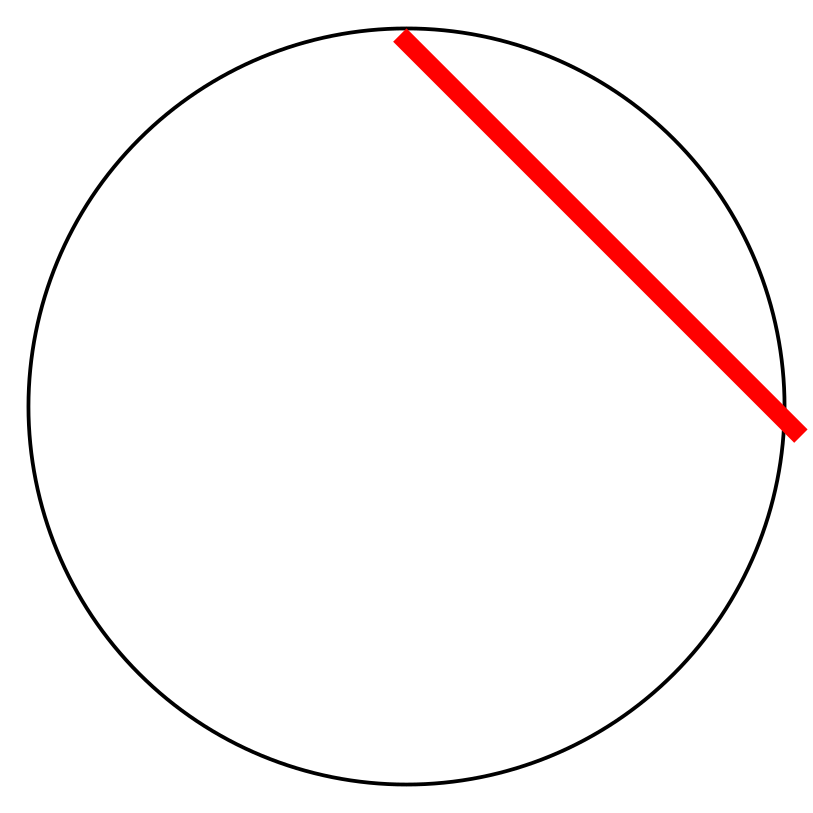
\includegraphics[width=0.35\textwidth]{spherical_approximations_line}
    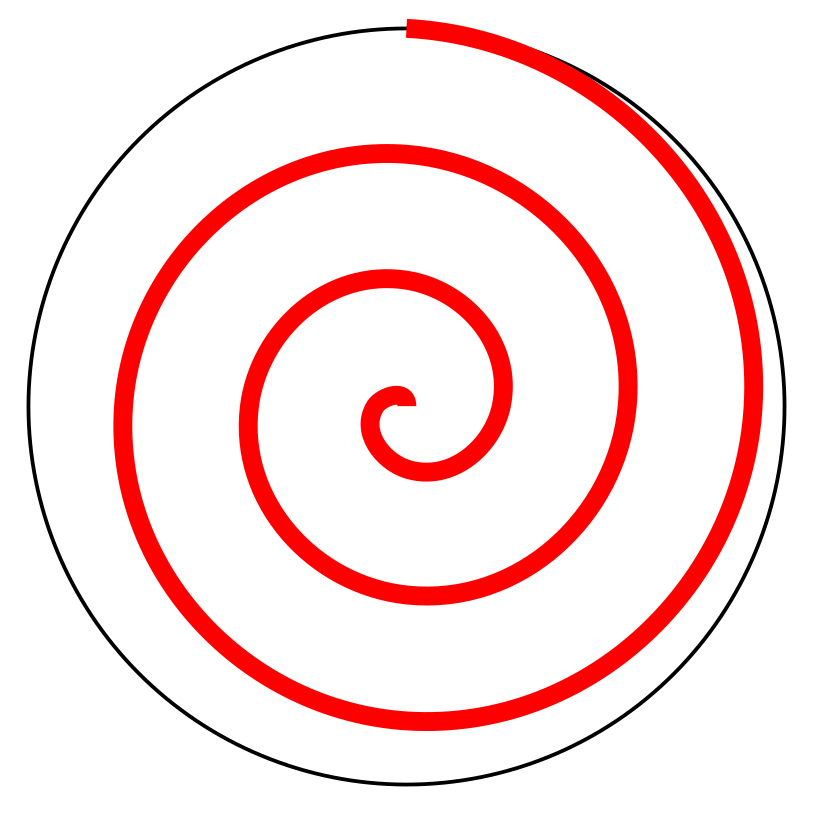
\includegraphics[width=0.35\textwidth]{spherical_approximations_spiral}
    \caption{Two possible interpretations of what a line with a constant angle in a spherical geometry could mean. On the left side a line with a constant angle (of 45 degrees) relative to the surface where it started. Although this is the most intuitive way of interpreting a plate going down with a certain dip, when using very long plates this means that the plate may go back out the earth again. Note that this will only happen with unrealistically long slabs and/or dips very close to zero. On the right side is the other interpretation, constant dip with resprect to the surface directly above it. This resutls in a logarithmic spiral.}
    \label{fig:coordinate_systems_line_spiral}
\end{figure}

\begin{remark}
Note that currently only the constant angle relative to the surface where it started (the left side of figure \ref{fig:coordinate_systems_line_spiral}).
\end{remark}

The first option (line) is simpler, more intuitive and makes no assumptions about what a slab should do within the earth. The second option (spiral) is less intuitive, 
but implicitly includes gravity in the slab. There are two more options, option three and four, which are a compromise between the first two. 
Both option three and four use the slab segments and recomputes the angle at the beginning of every segment. 
The third option of these two actually applies it directly at the beginning of the segment. This is most logical, but it can lead to discontiuities between two curved slab segments, 
even though they have the same ending and starting angle respectively.
The forth option applies the extra angle computed at the beginning of the segment to the end of the segment. This allows for a smmooth tranition and is generally recommended. 
With small enough segments, both these approximates the second (spiral) option. We have implemented the other options because the implementation of the spiral option has proven to 
be difficult and time consuming. 
So currently only the first, third and fourth option can be set through the \hl{depth method} parameter in the \hl{spherical} parameter, by setting the \hl{depth method} parameter 
to \hl{starting point}, \hl{begin point} and \hl{begin at end segment} respectively. 
Adding to the \WB{} file from the previous section by setting it to a spherical geometry, we get the following \WB{} file:

\begin{javascriptcode}{}{}
{
  "version":"0.5",
  "coordinate system":{"model":"spherical", "depth method":"starting point"},
  "features":[]
}
\end{javascriptcode}


\subsubsection{An endless world}
As you may have noticed, there are no bounds given to coordinate system extent. So how does the \WB{} know how big your model is? It doesn't, because it doesn't need to know. Both in Cartesian and spherical coordinates, the world is endless, with a small note that in spherical coordinates, entering 361 degrees longitude will yield the same position as 1 degree longitude. This doesn't mean that they can always be use interchangeably. But we will explain more on that in section \ref{section:continetnal_plate}. For now it is important to know that the \WB{} world knows no (spatial) limits.

\subsection{2d and 3d models}
The world we live in is an inherently 3d world, and so is the \WB{}. So no matter whether you are intending to use the \WB{} for a 2d or a 3d problem, you will need to define the 3d world. This doesn't mean that you can't use the \WB{} for 2d problems. On the contrary even, one of the core functionalities of the \WB{} are the 2d temperature and composition functions. The way this works is that you can define cross section through the 3d world. The cross section is given by providing the \hl{Cross section} parameter with two points on the surface. The first point will be the origin of the cross section, and the second point is the direction in which the cross section will be taken. Let's expand the Cartesian example from Listing \ref{lst:code_minimal_example_default_coordinate_system}, with a cross section:

\begin{javascriptcode}{An example showing how to use the cross section}{}
{
  "version":"0.5",
  "cross section":[[100e3,100e3],[400e3,500e3]],
  "coordinate system":{"model":"cartesian"},
  "features":[]
}
\end{javascriptcode}

The first thing you will notice is a first actual use of an array with the square brackets \hl{[ ]}. In this case it is an array, which contains two arrays, which each two numbers, i.e. it is an array of two 2d points. Remember from section \ref{section:coordinate_systems} that since we are using a Cartesian coordinate system, all the values have the unit meters. 

A second thing to note is that we are only using 2d surface coordinates to define a plane in 3d space. The reason we can do this is that we already know what the range of the 3rth coordinate needs to be: from the bottom of the model to the surface. So there is no need to let the user specify this.

When no cross section is given, the 3d functions of the \WB{} can be used without problems. When you want to set up a 2d model, make sure you have provided the cross section parameter with the correct surface coordinates.

\subsection{Plate tectonic features and models}
Before we can make our first real model, there is one more topic to discuss: features and models. As stated in the section on the idea behind the world builder (section \ref{section:idea_behind_WB}), we want users to be able to enter plate tectonic features and attach models to them to represent how certain properties, such as the temperature within that tectonic feature should be modeled. This is where the \hl{features} parameter comes into play. Through this parameter we can define the features and attach to them models for temperature and composition. In a generic way that looks something like this:

\begin{javascriptcode}{A example of a generic feature}{}
{
  "version":"0.5",
  "cross section":[[100e3,100e3],[400e3,500e3]],
  "coordinate system":{"model":"cartesian"},
  "features":
  [
    {
      "model":"feature model 1",
      "temperature models":[{"model":"temp. model 1"}],
      "composition models":[{"model":"comp. model 1"}]
    }
  ]
}
\end{javascriptcode}

A feature has a name and for every available property an array of models attached. Note that this example would not work in practice, because there is no feature implemented which is called \hl{feature model 1} or a temperature model with the name \hl{temperature model 1}. Only specific feature names are allowed, which will be introduced in section \ref{section:continetnal_plate} and can be found in the \WB{} input file parameter reference (see Appendix \ref{chapter:WB_file_parameter_reference}). Note that there is no requirement to have the temperature models or compositional models keys in the feature object. If you leave them out, they will just not do anything. Let's now expand the generic example:

\begin{javascriptcode}{A example of two generic features use}{}
{
  "version":"0.5",
  "cross section":[[100e3,100e3],[400e3,500e3]],
  "coordinate system":{"model":"cartesian"},
  "features":
  [
    {
      "model":"feature model 1",
      "temperature models":[{"model":"temp. model 1"}],
      "composition models":[{"model":"comp. model 1"}],
    },
    {
      "model":"feature model 2",
      "generic feature option 1":1000.0,
      "generic feature option 2":"value 2",
      "temperature models":[{"model":"temp. model 2", "temp. parameter":100e3}],
      "composition models":[{"model":"comp. model 2", "comp. parameter":1}]
    }
  ]
}
\end{javascriptcode}

Here we have added a second feature (again a non-existent feature). The second feature now has parameters which are set, and even the temperature and composition models have parameters which can be set. What is very important to know is that the order in which the features are listed matters. We haven't discussed the placing of features yet, but features may overlap, e.g. for one location, multiple features may be present. The list is read from top to bottom by the \WB{}, and every feature model receives the current value of the property in question. The specific model then returns a new value, which can be based on the value it received, but that doesn't have to be the case. 

\begin{remark}
The order in which the features are listed is important. It determines what happens when features overlap. In general it is a good rule to have the largest features at the top, and the smallest features at the bottom.
\end{remark}

This also means that there should be a starting value for each property. The starting value of the temperature is an adiabatic profile, of which the parameters can be set in the \WB{} input file. All the compositions start out with a value of zero.

\subsection{Naming and placing the features in the world}
There are two feature parameters which are required for every feature. The first one is the parameter \hl{name}. This is required to make sure that the \WB{} files remain readable. The name should indicate what the feature represents in the real world, or at least in the model. 

The second required parameter is the parameter is \hl{coordinates}. This is always an array of arrays of numbers, representing a list of 2d points on the surface. This list of 2d surface points can be interpreted by the features in three ways: an enclosed area, a line or a point. These determine three distinct type of features: area features, line features and point features. Examples of area features are a continental or oceanic plate. Examples of line features are subducting plates and faults. Although there are currently no point features implemented, one could think of a plume or a spherical anomaly as a point feature. Depending on the type of feature, the coordinates are interpreted differently, as is documented by the individual features. Here is our first generic example again, but now with the required parameters:

\begin{javascriptcode}{An example with a generic feature and the required parameters}{}
{
  "version":"0.5",
  "cross section":[[100e3,100e3],[400e3,500e3]],
  "coordinate system":{"model":"cartesian"},
  "features":
  [
    {
      "model":"feature model 1",
      "name":"Eurasia",
      "coordinates":[[0,0],[0,100e3],[200e3,100e3],[200e3,0]],
      "temperature models":[{"model":"temp. model 1"}],
      "composition models":[{"model":"comp. model 1"}],
    },
    {
      "model":"feature model 2",
      "name":"Africa",
      "coordinates":[[0,0],[0,-100e3],[-200e3,-100e3],[-200e3,0]],
      "generic feature option 1":1000.0,
      "generic feature option 2":"value 2",
      "temperature models":[{"model":"temp. model 2", "temp. parameter":100e3}],
      "composition models":[{"model":"comp. model 2", "comp. parameter":1}]
    }
  ]
}
\end{javascriptcode}

\begin{remark}
Note that a point feature can only have one point, a line features requires at least two points and an area features requires at least three points.
\end{remark}

\section{The continental plate}
\label{section:continetnal_plate}
\subsection{A basic continental plate}
We can now finally start building a useful geodynamic model. We begin with a continental plate, because this is probably the easiest feature. It is a type of feature where the coordinates define an area on the surface of the world. It has no additional requirements, so the most basic continental plate \WB{} file looks like this:

\begin{javascriptcode}[label=lst:simple_continental_plate]{An example of the most basic continental plate}{}
{
  "version":"0.5",
  "features":
  [
    {
      "model":"continental plate", "name":"Eurasia",
      "coordinates":[[0,0],[0,100e3],[200e3,100e3],[200e3,0]]
    }
  ]
}
\end{javascriptcode}

The example in listing \ref{lst:simple_continental_plate} is not yet functional since we need to attach temperature and compositional models to it. For the continental feature there are different models available. The simplest model for both temperature and composition are the uniform models. They set the temperature or a single compositions respectively to a specified value. In this case the only other paramter is the depth to which the continental plate goes. This is set by the \hl{depth} paramater in each models.

\begin{javascriptcode}{A first functioning continental plate example}{}
{
  "version":"0.5",
  "features":
  [
    {
      "model":"continental plate", "name":"Eurasia", "max depth":100e3,
      "coordinates":[[0,0],[0,100e3],[200e3,100e3],[200e3,0]],
      "temperature models":[{"model":"uniform", "temperature":293}],
      "composition models":
      [
        {"model":"uniform", "max depth":20e3, "compositions":[1]}
      ]
    }
  ]
}
\end{javascriptcode}

This code creates a continental plate which is 100 km thick which has a temperature of 293 K. In the first 20 km the composition with number 1 is present. Note that the compositions parameters is an array. Multiple compositions can be set through one composition model. When more then one composition is present, there is no need to set the fractions for each. The default value for fractions if there is just one composition is [1]. In the next example we show how to place two compositions in one feature, on with a fraction of 0.25 and one with a fraction of 0.75.
\begin{remark}
It is also possible to set a "min depth" for both the continental plate and the uniform models. In this case the default value of zero for min depth is good enough.
\end{remark}

\begin{javascriptcode}{A continental plate with two compositions with different fractions}{}
{
  "version":"0.5",
  "features":
  [
    {
      "model":"continental plate", "name":"Eurasia", "max depth":100e3,
      "coordinates":[[0,0],[0,100e3],[200e3,100e3],[200e3,0]],
      "temperature models":[{"model":"uniform", "temperature":293}],
      "composition models":
      [
        {
          "model":"uniform", "max depth":20e3, "compositions":[1,4], 
          "fractions":[0.25,0.75]
        }
      ]
    }
  ]
}
\end{javascriptcode}

We have stated before that temperature and composition models get the previous tempeature or compostional value respectively, and that each model can decide wheter to use that value or not. Many temperature models give the option to the user. This is also the case with the uniform temperature models for the continental plate. By default it replaces the value, but the it can also be added or substracted. This is set with the operation key. Let's do that now, but do that in a second temperature model in the array.

\begin{javascriptcode}{A continental plate with an add operation for the temperature model}{}
{
  "version":"0.5",
  "features":
  [
    {
      "model":"continental plate", "name":"Eurasia", "max depth":100e3,
      "coordinates":[[0,0],[0,100e3],[200e3,100e3],[200e3,0]],
      "temperature models":
      [
        {"model":"uniform", "temperature":293},
        {"model":"uniform", "temperature":1, "operation":"add"}
      ],
      "composition models":
      [
        {
          "model":"uniform", "max depth":20e3, "compositions":[1,4], 
          "fractions":[0.25,0.75]
        }
      ]
    }
  ]
}
\end{javascriptcode}

\begin{remark}
There is no fundamental reason why the compositional uniform model doesn't have an add operation, except that it hasn't been implemented yet.
\end{remark}

\subsection{linear temperature profile and layers}
Continents with a constant temperature and composition are obviously not very realistic. The next step we can take is prescribing a linear temperature gradient with depth. The \hl{linear} temperature model is then used. This temperature model has one required and four optional parameters. The required parameter is the \hl{max depth}. The optional parameters are the \hl{min depth} (default 0), the \hl{top temperature} (default 293) and the \hl{bottom temperature} (default -1). The negative default value for the bottom temperature might seem odd for a temperature. In this temperature model, if the temperature is negative, it is replaced with an adiabatic temperature at the depth of min depth for the top temperature and at max depth for the bottom temperature. So the default is a linear temperature profile from the surface with surface temperature to a user-specified depth with an adiabatic temperature at that depth.

\begin{javascriptcode}{Using the linear temperature model}{}
{
  "version":"0.5",
  "features":
  [
    {
      "model":"continental plate", "name":"Eurasia", "max depth":100e3,
      "coordinates":[[0,0],[0,100e3],[200e3,100e3],[200e3,0]],
      "temperature models":[{"model":"linear", "max depth":100e3}],
      "composition models":
      [
        {"model":"uniform", "max depth":20e3, "compositions":[1]}
      ]
    }
  ]
}
\end{javascriptcode}

We can also improve the compositional representation through having multiple compositional models in a single feature. This allows us to for example have a separate composition for the upper crust, lower crust and the rest of the plate.

\begin{javascriptcode}{Using the linear temperature model}{}
{
  "version":"0.5",
  "features":
  [
    {
      "model":"continental plate", "name":"Eurasia", "max depth":100e3,
      "coordinates":[[0,0],[0,100e3],[200e3,100e3],[200e3,0]],
      "temperature models":[{"model":"linear", "max depth":100e3}],
      "composition models":
      [
        {"model":"uniform", "max depth":20e3, "compositions":[0]},
        {"model":"uniform", "min depth":20e3, "max depth":50e3, "compositions":[1]},
        {"model":"uniform", "min depth":50e3, "max depth":100e3, "compositions":[2]}
      ]
    }
  ]
}
\end{javascriptcode}

The first layer is the top layer, which reaches a depth of 20 km. The second layer starts from 20 km and reaches 50 km. The third layer starts at 50 km and ends at 100km. In this case the order does not really matter because there is no overlap. In case of overlap between the models, the order works the same way as it does for the features, it is drawn from top to bottom.

\begin{remark}
Note that any layer beyond the continental plate depth is ignored. So in this case if we made the third layer max depth 120 km, the results would still be the same.
\end{remark}

With this you are now able to create your own continents. Congratulations and well done for reaching this point in the manual! Next up are Oceanic plates.

\section{The oceanic plate}
Oceanic plates are very similair to continental plates, with the exeption of the extra model: the \hl{plate model}. This name may sound confusing, since we have been talking about plates all the time. The reason we use this name is that this is the name commonly used in the geodynamics community, see for example \cite{fowler2005}. 

This temperature model takes exactly the same parameters as the linear temperature model, but has two more parameters. The first one is the \hl{spreading velocity} in meters per second. The second one is a list of 2d points where the ridge is located. From the ridge defined by these points, the plate will symmetrically cool on each side.

\begin{javascriptcode}{Using the oceanic plate's "plate model" temperature model}{}
{
  "version":"0.5",
  "features":
  [
    {
      "model":"oceanic plate", "name":"Eurasia", "max depth":100e3,
      "coordinates":[[0,0],[0,100e3],[200e3,100e3],[200e3,0]],
      "temperature models":
      [
        {
          "model":"plate model", "max depth":100e3, "plate velocity":0.01,
          "ridge points":[[50e3,0],[50e3,50e3],[100e3,100e3]]
        }
      ],
      "composition models":
      [
        {"model":"uniform", "max depth":20e3, "compositions":[0]}
      ]
    }
  ]
}
\end{javascriptcode}

\section{The mantle layer}
The \WB{} supports layering of the mantle. Teh mantle layer feature follows the same logic as the continental and oceanic plate. An example of a different compositional layer at the 660 is given in listing \ref{listing_mantle_layer_different_composition}.

\begin{javascriptcode}{Using the oceanic plate's "plate model" temperature model}{listing_mantle_layer_different_composition}
{
  "version":"0.5",
  "features":
  [
    {
      "model":"mantle layer", "name":"660 phase change", "max depth":100e3,
      "coordinates":[[0,0],[0,100e3],[200e3,100e3],[200e3,0]],
      "composition models":
      [
        {"model":"uniform", "max depth":100e3, "compositions":[0]}
        {"model":"uniform", "min depth":100e3, "max depth":1000e3, "compositions":[1]}
      ]
    }
  ]
}
\end{javascriptcode}

\section{The subducting plate}
While the continental plate, the oceanic plate and the mantle layer are all area features, we now come across the first line feature: the subducting plate. This means that the coordinates defined in this feature do not form an area on the surface, which we extrapolate into the depth, but instead it represents the intersection between the plane and the surface. Beside the two normal required parameters, this feature requires at least two more parameters to be specified. The first one is called the \hl{dip point}. In simple terms, a subducting plate, with a angle between 0 and 90 degrees, will always point in the general direction of the location of this point. The second parameter is the called \hl{segments}. The way this parameter works is best explained by an example. Let's make for our first slab a slab which goes down with an angle of 45 degrees, is 200 km long and 100 km thick.

\begin{javascriptcode}{Using the subducting plate constant segment}{}
{
"version":"0.5",
"features":
[
     {
       "model":"subducting plate", "name":"Antilles slab", "dip point":[1e7,-1e7],
       "coordinates":[[0,0],[50e3,50e3]], 
       "segments":[{"length":200e3, "thickness":[100e3], "angle":[45]}]
    }
}
\end{javascriptcode}

Segments have three required values and two optional. Let's first discuss the required options. The required options are the length, an array with one or two thicknesses and an array with one or two angles (in degrees). The arrays for the thickness and angle can be used to let that value change (linearly) from the beginning of the segment to the end of the segment. The following example changes the thickness from 100km to 50km and the angle from 0 degree to 45 degrees along the 200km length. We also add a second segment which is 400km long and where the angle changes from 45 degrees back to 0 degree. To be able to visualize this we also add a cross section and a composition and temperature model. The result is shown in figure \ref{fig:simple_2d_subduction_1}.

\begin{javascriptcode}{Using the subducting plate changing segment}{lst_json:simple_2d_subduction}
{
  "version":"0.5",
  "cross section":[[0,50e3],[50e3,0]],
  "features":
  [
     {
       "model":"subducting plate", "name":"Antilles slab", "dip point":[1e7,-1e7],
       "coordinates":[[0,0],[50e3,50e3]], 
       "segments":
       [
         {"length":200e3, "thickness":[100e3, 50e3], "angle":[0,45]},
         {"length":400e3, "thickness":[50e3, 100e3], "angle":[45,0]}
       ],
       "temperature models":[{"model":"uniform", "temperature":600}],
       "composition models":[{"model":"uniform", "compositions":[0]}]
    }
  ]
}
\end{javascriptcode}

\begin{figure}
    \centering
    \includegraphics[width=0.99\textwidth]{simple_subducting_plate_example.png}
    \caption{A slab produced by Listing \ref{lst_json:simple_2d_subduction}, where the red indicates the position of the slab}
    \label{fig:simple_2d_subduction_1}
\end{figure}

Now rises the question, what if you want to give the second segment a different compositions, or even a layered composition? This is where the two optional segment options come into play. These are \hl{compositional models} and \hl{temperature models}. The composition (and temperature) models given in top feature just act as a default composition model, but if you want something different in a segment, you only need to define it. To make different layers in a subducting slab we have to use \hl{min distance slab top} and \hl{max distance slab top} instead of \hl{min depth} and \hl{max depth}, because we want to define a layer in a curved slab. Let's now combine these two new pieces of information into a more interesting model.

\begin{javascriptcode}{Using the subducting plate changing segment}{lst_json:simple_2d_subduction_layered_second_segment}
{
  "version":"0.5",
  "cross section":[[0,50e3],[50e3,0]],
  "features":
  [
     {
       "model":"subducting plate", "name":"Antilles slab", "dip point":[1e7,-1e7],
       "coordinates":[[0,0],[50e3,50e3]], 
       "segments":
       [
         {"length":200e3, "thickness":[100e3, 50e3], "angle":[0,45]},
         {
           "length":400e3, "thickness":[50e3, 100e3], "angle":[45,0],
           "composition models":
           [
             {"model":"uniform", "compositions":[1], "max distance slab top":30e3},
             {"model":"uniform", "compositions":[1], "min distance slab top":30e3}
           ]
         }
       ],
       "temperature models":[{"model":"uniform", "temperature":600}],
       "composition models":[{"model":"uniform", "compositions":[0]}]
    }
  ]
}
\end{javascriptcode}


\begin{figure}
    \centering
    \includegraphics[width=0.99\textwidth]{simple_subducting_plate_example_segments.png}
    \caption{A slab produced by Listing \ref{lst_json:simple_2d_subduction_layered_second_segment}, where the red indicates the position of the first segment of the slab slab, the green indicates the top 20 km of the second segment of the slab, and the yellow shows the lower part of the second segment of the slab.}
    \label{fig:simple_2d_subduction_2}
\end{figure}

Although this is already an interesting model things might not only change down dip, but also along the trench. To explain how this is facilitated, let's first introduce a new term: sections. Sections are slices in the dip direction of the slab, and may consist of several segments. Each coordinate given by the user forms a section. All properties are computed for the two sections closed to the point we are requesting the data for and then we make a linear interpolation between those sections. By default all the sections of a slab are filled with the segments by the segments parameter. So if we want to change for example the temperature along the trench, we only need to change one of the sections. This is done through the sections parameter, which has as value an array of subducting plate features. The only difference is that you don't need (nor can) use the model parameter, because it has to be a subducting plate, and you have to provide the coordinate number which you want to change. In text that may more more complated then it is, so lets show extend the example a bit with some different sections.

\begin{javascriptcode}{Using the subducting plate changing segment}{lst_json:simple_2d_subduction_layered_second_segment_sections}
{
  "version":"0.5",
  "cross section":[[0,99e3],[99e3,0]],
  "features":
  [
     {
       "model":"subducting plate", "name":"Antilles slab", "dip point":[1e7,-1e7],
       "coordinates":[[0,0],[50e3,50e3]],
       "segments":
       [
         {"length":200e3, "thickness":[100e3, 50e3], "angle":[0,45]},
         {
           "length":400e3, "thickness":[50e3, 100e3], "angle":[45,0],
           "composition models":
           [
             {"model":"uniform", "compositions":[1], "max distance slab top":30e3},
             {"model":"uniform", "compositions":[2], "min distance slab top":30e3}
           ]
         }
       ],
       "sections":
       [
         {
           "coordinate":1,
           "segments":
            [
              {"length":200e3, "thickness":[100e3, 50e3], "angle":[0,45]},
              {"length":400e3, "thickness":[50e3, 100e3], "angle":[45,0], 
                "temperature models":[{"model":"uniform", "temperature":650}]}
            ],
            "temperature models":[{"model":"linear", "max distance slab top":100e3, 
                                     "top temperature":650, "bottom temperature":550}]
         }
       ],
       "temperature models":[{"model":"uniform", "temperature":600}],
       "composition models":[{"model":"uniform", "compositions":[0]}]
    }
  ]
}
\end{javascriptcode}

\begin{figure}
    \centering
    \includegraphics[width=0.99\textwidth]{manual_subduction_section_segments_dist_all_v3_small.png}
    \caption{Three cross sections of the temperature and composition fields of slab produced by Listing \ref{lst_json:simple_2d_subduction_layered_second_segment_sections}. Distance is in km.}
    \label{fig:simple_2d_subduction_3}
\end{figure}

The example in listing \ref{lst_json:simple_2d_subduction_layered_second_segment_sections} shows that an enormous amount of flexibility is available, but only to those who really need it. If you want something simple, your input file will be simple.

The subducting plate has, like the oceanic plate, a special temperature model. This is also called the plate model. It it based on the \cite{mckenzie1970} paper. Because that paper assumes a constant angle, and the slabs in the \GWB{} are not constant, we compute an average angle at the depth we are currently intrested in. Lets combine everything we know up to now and create a more realistic slab with a crust an a plate model. Feel free to visualize this yourself through the world builder visualizer or any other program.

\begin{javascriptcode}{Using the subducting plate changing segment}{lst_json:simple_2d_subduction_layered_second_segment}
{
  "version":"0.5",
  "cross section":[[0,50e3],[50e3,0]],
  "features":
  [
     {
       "model":"subducting plate", "name":"Antilles slab", "dip point":[1e7,-1e7],
       "coordinates":[[0,0],[50e3,50e3]], 
     "segments":
     [
         {"length":200e3, "thickness":[100e3, 50e3], "angle":[0,45]},
         {"length":400e3, "thickness":[50e3, 100e3], "angle":[45,0]}
     ],
     "temperature models":
     [
       {"model":"plate model", "density":3300, "plate velocity":0.01}
     ],
     "composition models":
     [
       {"model":"uniform", "compositions":[0], "max distance slab top":10e3},
       {"model":"uniform", "compositions":[1], "min distance slab top":10e3}
     ]
    }
  ]
}
\end{javascriptcode}


\section{Faults}
Fault in the \WB{} work in a very similar way as subducting plates. The mayor difference is that where subducting plates measure distance based on the top of the plate, faults measure from the center of the fault. This means that faults modules are usually symmetric. For example, the \hl{uniform} composition model askes for min and max distance from fault center instead of slab top as with the subducting plate feature. This make faults symmetric around the center. Note that the thickness of the central layer is twice the max distance fault center, because it goes in both directions.

\begin{javascriptcode}{Using the fault feature}{}
"version":"0.5",
"features":
{
  {
    "model":"fault", "name":"none fault",  "dip point":[0,-1],
    "coordinates":[[0e3,250e3],[500e3,250e3],[1000e3,500e3]],
    "segments":
    [
      {"length":200e3, "thickness":[100e3,90e3], "angle":[0,45]}, 
      {"length":200e3, "thickness":[90,80], "angle":[45,60]}, 
      {"length":150e3, "thickness":[80], "angle":[60,0]}
    ],
    "temperature models":[{"model":"uniform", "temperature":100e3}],
    "composition models":
    [
      {"model":"uniform", "compositions":[0], "max distance fault center":16.5e3},
      {"model":"uniform", "compositions":[1], "min distance fault center":16.5e3, 
        "max distance fault center":33e3},
      {"model":"uniform", "compositions":[2,3], "fractions":[0.25,0.75], 
         "min distance fault center":33e3}
    ]
  }
}
\end{javascriptcode}

\section{Cookbooks}
Up to now we have shows several features in isolation, but the \WB{} is designed to combine those features together to one integrated model. How this is done is shown in the cookbooks in the cookbook directory.

\section{Using the World Builder App}
\label{section:using_the_app}
This is a program which can be used to query the \WB{} from the command line, by providing it a world builder file, and then a data file. This data file should contain in the header information on the dimension you want to use and the amount of compositions, and in the main part the required information like for example for a 3d case x,y and z position, depth and gravity (See Listing \ref{lst:code_example_app_input_data_file}). The output of the data file from listing \ref{lst:code_example_app_input_data_file},, with a certain \WB{} file, is presented in Listing \ref{lst:code_example_app_out}.

\begin{bashcode}[label={lst:code_example_app_input_data_file}]{Example input data file}
# This is a comment in the data
# file. 
# Now define parameters:
# dim = 2
# compositions = 5
# x      z d g  T c1 c2 c3 c4 c5
  1      2 2 10
  2      2 2 10
  3      4 0 10
  560e3  0 0 10
  1999e3 0 0 10
\end{bashcode}

\begin{bashcode}[label={lst:code_example_app_out}]{Example output from above input for the \WB{} app}
# x z d T c0 c1 c2 c3 c4 
1 2 2 10 1600 0 0 0 0 0 
2 2 2 10 1600 0 0 0 0 0 
3 4 0 10 1600 0 0 0 0 0 
560e3 0 0 10 150 0 0 0 1 0 
2000e3 0 0 10 20 0 0 1 0 0
\end{bashcode}

\section{Using the World Builder Visualizer}
\label{section:using_the_visualizer}
This program helps with visualizing the \WB{} file by producing pvd files which can be opened with visualization programs like \paraview{}. It requires a \WB{} file and a grid file. A grid file is a file which contains information about what part of the \WB{} domain should be visualized. An example of a grid file can be found in Listing \ref{lst:code_example_grid_file}.

\begin{bashcode}[label={lst:code_example_grid_file}]{An example of a grid file for a 3d Cartesian grid.}
# ouput variables
grid_type = cartesian
dim = 3
compositions = 2

# domain of the grid
x_min = 0e3
x_max = 2000e3
y_min = 0e3
y_max = 1000e3
z_min = 0 
z_max = 750e3

# grid properties
n_cell_x = 160
n_cell_y = 80
n_cell_z = 60
\end{bashcode}

\section{Final comments}
There you have it, all the basics of the \GWB{}! You have seen how each component of the \WB{} works, and how the ideas are implemented. But in the end the best way to learn and to find out what the \WB{} is really capable of is to just try it out. If stumble on a problem or think that something should work differently or even that you really need a specific functionality, don't stay silent. Please let it know on github: \url{https://github.com/GeodynamicWorldBuilder/WorldBuilder}. Feel free to make an issue, so that your problem or idea can be discussed. 
\\
We are also happy if you want to contribute code or documentation. If you find a mistake in the manual or code, even is it is a simple spelling or grammatical mistake, please report it. The effort is really appreciated. It would also make for a great first pull request!




\part{Information for developing for the World Builder}
\chapter{Introduction}
\section{prerequisites}
To contribute to the world builder there the only prerequisites is that you are willing to contriube to open-source software under the GNU LESSER GENERAL PUBLIC LICENSE version 2.1. See the licence document in the repository for more information. As mentioned in part 1 of the manual, we really appreciate any contribution!

If you want to contribute code, some knowledge of of c++ is required. For writing and changing plugins, a basic knowledge of how variables, loops and functions work should be sufficient to be able to contribute. 

As a version management system, and also as a system to manage and discuss contributions, we use git and github. Some basic knowledge on how git works will speed up how fast you can contribute to the \WB{}.

If there is something you do not understand, do not hesitate to ask a question by making a issue on github.

\section{Conventions}
There are several conversions used when writing code. Because the code is still very young, we will only name the most important ones. 
\begin{enumerate}
    \item all parameters in the \WB{} parameter file are lower case.
    \item all variable names are snake case (variable\_name).
    \item all function names are snake case (function\_name).
    \item all class names are camel case (ClassName).
\end{enumerate}
\chapter{Structure and flow of the code}
From version 0.2.0 to version 0.3.0 the structure has mostly been stabelized. On a high level the structure is very similair to that of \aspect{}, 
with an extensive modular plugin system. Also the way to declare and parse parameters is very similair to \aspect{} and DEAL.II. Besides being a 
good and proven strucutre for these kind of codes, these similairities are also on propose to allow for an easy transition for \WB{} and \aspect{}
developers between the codes. This is also reflected in having similair conventions and the use of exactly the same indenting tool and version 
astyle (2.04). 

The \GWB{} currently consists of three parts: the core library, the App and the Visualizer. The App and Visualizer are self contained
with their own main program and use the core library. The core library has a includes/world\_builder folder and a source folder containing
all the header files and source files respectively. The source folder contains three folders and several files. The files in this folder are a 
combination of core files glueing the WB together, configuration files and wrapper files the for the interfaces to different programming languages.
The most important files here are world.cc and parameters.cc. The file world.cc contains the world class which other programs use to interact with 
the world builder library. The parameters.cc file contains the Parameters class which deals with loading and parsing the world builder file (.wb). 
The load and parsing process is quite involved, but the high level version of it is that the core files and each plugin declares what parameters are 
available and what values are allowed for that parameter. These declarations build a JSON schema (Remember that the world builder files use JSON syntax).
Then this schema is used to see if the provided world builder file is valid according to that schema. If the world builder file passes the schema check 
phase, the actual parsing phase starts. This means that the core files and plugins will load the information in the world builder file into memory and
can perform extra checks on those values. After this phase is done, the plugins do not have access anymore to the parameters class. This is also the 
last pahse of the construction of the world class.

The three folders contain plugin systems. Writing a new plugin for the coordinate system and types is as easy as copying an exsiting plugin (both in the 
include and source folders!) and modifying it for your own purposes. The plugins in the features plugin system are a bit more complicated since they have 
their owns plugin systems. If you want tomake a whole new feature you are adviced to make an issue on github so that you can get help with it from the 
developers and to allow discussion on the best approach. The features folder contains a folder for each features plugin (system). Each of those folders 
contains a folder for the output provided by the world builder. That is at time of writing temperature, compositions and grains (experimental). Eeach of 
those folders contains an interface file and at least one plugin. Adding a new plugin is, like with the coordinate and types plugins as easy as copying 
and modifing one of those plugins (again, you need to do that for both the include and source files. So if you want to for example add a new temperature 
plugin for the oceanic plate plugin system called "my cool oceanic plate temperature", you could copy the plate\_model.cc to my\_cool\_temperature.cc and 
uniform.h to my\_cool\_temperature.h in their respective folders. You will need to change plate\_model to my\_cool\_temperature, PlateModel to MyCoolTemperature,
etc.

In depth question of the structure and flow of the code can always be asked on github as an issue.
%\chapter*{Bibliography}
\bibliographystyle{apalike}
\bibliography{bibliography}
\addcontentsline{toc}{chapter}{\textcolor{ocre}{Bibliography}}

\appendix
\chapter{\WB{} file parameter reference}
%\setlistdepth{15}
\label{chapter:WB_file_parameter_reference}
\section{/}
\begin{itemize}\item {\bf type}: object
\item {\bf documentation}: Root object
\item {\bf additionalProperties}: false
\item {\bf required}: [version, features]\end{itemize}
\section{/version}
\begin{itemize}\item {\bf default value}: 
\item {\bf type}: string
\item {\bf documentation}: The major and minor version number for which the input file was written.
\end{itemize}\section{/cross section}
\begin{itemize}\item {\bf type}: array
\item {\bf minItems}: 2
\item {\bf maxItems}: 2
\item {\bf uniqueItems}: false
\item {\bf documentation}: This is an array of two points along where the cross section is taken
\end{itemize}\section{/cross section/items}
\begin{itemize}\item {\bf type}: array
\item {\bf minItems}: 2
\item {\bf maxItems}: 2
\item {\bf documentation}: 
\end{itemize}\subsection{/cross section/items/items}
\begin{itemize}\item {\bf type}: number
\end{itemize}\section{/potential mantle temperature}
\begin{itemize}\item {\bf default value}: 1600.0
\item {\bf type}: number
\item {\bf documentation}: The potential temperature of the mantle at the surface in Kelvin.
\end{itemize}\section{/surface temperature}
\begin{itemize}\item {\bf default value}: 293.15
\item {\bf type}: number
\item {\bf documentation}: The temperature at the surface in Kelvin.
\end{itemize}\section{/force surface temperature}
\begin{itemize}\item {\bf default value}: false
\item {\bf type}: boolean
\item {\bf documentation}: Force the provided surface temperature to be set at the surface
\end{itemize}\section{/thermal expansion coefficient}
\begin{itemize}\item {\bf default value}: 0.000035
\item {\bf type}: number
\item {\bf documentation}: The thermal expansion coefficient in $K^{-1}$.
\end{itemize}\section{/specific heat}
\begin{itemize}\item {\bf default value}: 1250.0
\item {\bf type}: number
\item {\bf documentation}: The specific heat in $J kg^{-1} K^{-1}.$
\end{itemize}\section{/thermal diffusivity}
\begin{itemize}\item {\bf default value}: 8.04e-7
\item {\bf type}: number
\item {\bf documentation}: The thermal diffusivity in $m^{2} s^{-1}$.
\end{itemize}\section{/maximum distance between coordinates}
\begin{itemize}\item {\bf default value}: 0.0
\item {\bf type}: number
\item {\bf documentation}: This enforces a maximum distance (in degree for spherical coordinates or meter in cartesian coordinates) between coordinates in the model. If the distance is larger, extra points are added by interpolation. Requires interpolation to be not 'none'.
\end{itemize}\section{/interpolation}
\begin{itemize}\item {\bf default value}: none
\item {\bf type}: string
\item {\bf documentation}: What type of interpolation should be used to enforce the minimum points per distance parameter. Options are none, linear, monotone spline and continuous monotone spline interpolation.
\end{itemize}\section{/coordinate system}
\begin{itemize}\item {\bf documentation}: A coordinate system. Cartesian or spherical.
\item {\bf default value}: cartesian
\item {\bf type}: object
\end{itemize}
\section{/coordinate system/oneOf/1}
\begin{itemize}\item {\bf type}: object
\item {\bf documentation}: Coordinate system object
\item {\bf additionalProperties}: false
\item {\bf required}: [model]\end{itemize}
\subsection{/coordinate system/oneOf/1/model}
\begin{itemize}\item {\bf default value}: 
\item {\bf type}: string
\item {\bf documentation}: The name which the user has given to the feature.
\item {\bf enum}: [cartesian]\end{itemize}\section{/coordinate system/oneOf/2}
\begin{itemize}\item {\bf type}: object
\item {\bf documentation}: Coordinate sysetm object
\item {\bf additionalProperties}: false
\item {\bf required}: [model, depth method]\end{itemize}
\subsection{/coordinate system/oneOf/2/model}
\begin{itemize}\item {\bf default value}: 
\item {\bf type}: string
\item {\bf documentation}: The name which the user has given to the feature.
\item {\bf enum}: [spherical]\end{itemize}\subsection{/coordinate system/oneOf/2/depth method}
\begin{itemize}\item {\bf default value}: 
\item {\bf type}: string
\item {\bf documentation}: Which depth method to use in the spherical case. The available options are 'starting point' and 'begin segment'.
\item {\bf enum}: [starting point, begin segment, continuous]\end{itemize}\section{/features}
\begin{itemize}\item {\bf documentation}: A list of features.
\item {\bf default value}: 
\item {\bf type}: array
\end{itemize}\section{/features/items}

\subsection{/features/items/oneOf/1}
\begin{itemize}\item {\bf type}: object
\item {\bf documentation}: continental plate object
\item {\bf additionalProperties}: false
\item {\bf required}: [model, coordinates]\end{itemize}
\subsection{/features/items/oneOf/1/model}
\begin{itemize}\item {\bf default value}: 
\item {\bf type}: string
\item {\bf documentation}: The name which the user has given to the feature.
\item {\bf enum}: [continental plate]\end{itemize}\subsection{/features/items/oneOf/1/name}
\begin{itemize}\item {\bf default value}: 
\item {\bf type}: string
\item {\bf documentation}: The name which the user has given to the feature.
\end{itemize}\subsection{/features/items/oneOf/1/coordinates}
\begin{itemize}\item {\bf type}: array
\item {\bf minItems}: 1
\item {\bf maxItems}: 4294967295
\item {\bf uniqueItems}: false
\item {\bf documentation}: An array of 2d Points representing an array of coordinates where the feature is located.
\end{itemize}\subsection{/features/items/oneOf/1/coordinates/items}
\begin{itemize}\item {\bf type}: array
\item {\bf minItems}: 2
\item {\bf maxItems}: 2
\item {\bf documentation}: 
\end{itemize}\subsubsection{/features/items/oneOf/1/coordinates/items/items}
\begin{itemize}\item {\bf type}: number
\end{itemize}\subsection{/features/items/oneOf/1/interpolation}
\begin{itemize}\item {\bf default value}: global
\item {\bf type}: string
\item {\bf documentation}: What type of interpolation should be used to enforce the minimum points per distance parameter. Options are global, none, linear, monotone spline and continuous monotone spline interpolation. If this value is set to global, the global value for interpolation is used.
\end{itemize}\subsection{/features/items/oneOf/1/min depth}
\begin{itemize}\item {\bf default value}: 0.0
\item {\bf type}: number
\item {\bf documentation}: The depth to which this feature is present
\end{itemize}\subsection{/features/items/oneOf/1/max depth}
\begin{itemize}\item {\bf default value}: 1.7976931348623157e308
\item {\bf type}: number
\item {\bf documentation}: The depth to which this feature is present
\end{itemize}\subsection{/features/items/oneOf/1/temperature models}
\begin{itemize}\item {\bf documentation}: A list of temperature models.
\item {\bf default value}: 
\item {\bf type}: array
\end{itemize}\subsection{/features/items/oneOf/1/temperature models/items}

\subsubsection{/features/items/oneOf/1/temperature models/items/oneOf/1}
\begin{itemize}\item {\bf type}: object
\item {\bf documentation}: temperature object
\item {\bf additionalProperties}: false
\item {\bf required}: [model]\end{itemize}
\subsubsection{/features/items/oneOf/1/temperature models/items/oneOf/1/model}
\begin{itemize}\item {\bf default value}: 
\item {\bf type}: string
\item {\bf documentation}: The name of the temperature model.
\item {\bf enum}: [adiabatic]\end{itemize}\subsubsection{/features/items/oneOf/1/temperature models/items/oneOf/1/operation}
\begin{itemize}\item {\bf default value}: replace
\item {\bf type}: string
\item {\bf documentation}: Whether the value should replace any value previously defined at this location (replace), add the value to the previously define value (add) or subtract the value to the previously define value (subtract).
\item {\bf enum}: [replace, add, subtract]\end{itemize}\subsubsection{/features/items/oneOf/1/temperature models/items/oneOf/1/min depth}
\begin{itemize}\item {\bf default value}: 0.0
\item {\bf type}: number
\item {\bf documentation}: The depth in meters from which the temperature of this feature is present.
\end{itemize}\subsubsection{/features/items/oneOf/1/temperature models/items/oneOf/1/max depth}
\begin{itemize}\item {\bf default value}: 1.7976931348623157e308
\item {\bf type}: number
\item {\bf documentation}: The depth in meters to which the temperature of this feature is present.
\end{itemize}\subsubsection{/features/items/oneOf/1/temperature models/items/oneOf/1/potential mantle temperature}
\begin{itemize}\item {\bf default value}: -1.0
\item {\bf type}: number
\item {\bf documentation}: The potential temperature of the mantle at the surface in Kelvin. If the value is lower then zero, the global value is used.
\end{itemize}\subsubsection{/features/items/oneOf/1/temperature models/items/oneOf/1/thermal expansion coefficient}
\begin{itemize}\item {\bf default value}: -1.0
\item {\bf type}: number
\item {\bf documentation}: The thermal expansion coefficient in $K^{-1}$. If the value is lower then zero, the global value is used.
\end{itemize}\subsubsection{/features/items/oneOf/1/temperature models/items/oneOf/1/specific heat}
\begin{itemize}\item {\bf default value}: -1.0
\item {\bf type}: number
\item {\bf documentation}: The specific heat in $J kg^{-1} K^{-1}$. If the value is lower then zero, the global value is used.
\end{itemize}\subsubsection{/features/items/oneOf/1/temperature models/items/oneOf/2}
\begin{itemize}\item {\bf type}: object
\item {\bf documentation}: Temperature model object
\item {\bf additionalProperties}: false
\item {\bf required}: [model, max depth]\end{itemize}
\subsubsection{/features/items/oneOf/1/temperature models/items/oneOf/2/model}
\begin{itemize}\item {\bf default value}: 
\item {\bf type}: string
\item {\bf documentation}: The name of the temperature model.
\item {\bf enum}: [linear]\end{itemize}\subsubsection{/features/items/oneOf/1/temperature models/items/oneOf/2/operation}
\begin{itemize}\item {\bf default value}: replace
\item {\bf type}: string
\item {\bf documentation}: Whether the value should replace any value previously defined at this location (replace), add the value to the previously define value (add) or subtract the value to the previously define value (subtract).
\item {\bf enum}: [replace, add, subtract]\end{itemize}\subsubsection{/features/items/oneOf/1/temperature models/items/oneOf/2/min depth}
\begin{itemize}\item {\bf default value}: 0.0
\item {\bf type}: number
\item {\bf documentation}: The depth in meters from which the temperature of this feature is present.
\end{itemize}\subsubsection{/features/items/oneOf/1/temperature models/items/oneOf/2/max depth}
\begin{itemize}\item {\bf default value}: 1.7976931348623157e308
\item {\bf type}: number
\item {\bf documentation}: The depth in meters to which the temperature of this feature is present.
\end{itemize}\subsubsection{/features/items/oneOf/1/temperature models/items/oneOf/2/top temperature}
\begin{itemize}\item {\bf default value}: 293.15
\item {\bf type}: number
\item {\bf documentation}: The temperature at the top in degree Kelvin of this feature.If the value is below zero, the an adiabatic temperature is used.
\end{itemize}\subsubsection{/features/items/oneOf/1/temperature models/items/oneOf/2/bottom temperature}
\begin{itemize}\item {\bf default value}: -1.0
\item {\bf type}: number
\item {\bf documentation}: The temperature at the top in degree Kelvin of this feature. If the value is below zero, an adiabatic temperature is used.
\end{itemize}\subsubsection{/features/items/oneOf/1/temperature models/items/oneOf/3}
\begin{itemize}\item {\bf type}: object
\item {\bf documentation}: Temperature model object
\item {\bf additionalProperties}: false
\item {\bf required}: [model, temperature]\end{itemize}
\subsubsection{/features/items/oneOf/1/temperature models/items/oneOf/3/model}
\begin{itemize}\item {\bf default value}: 
\item {\bf type}: string
\item {\bf documentation}: The name of the temperature model.
\item {\bf enum}: [uniform]\end{itemize}\subsubsection{/features/items/oneOf/1/temperature models/items/oneOf/3/operation}
\begin{itemize}\item {\bf default value}: replace
\item {\bf type}: string
\item {\bf documentation}: Whether the value should replace any value previously defined at this location (replace), add the value to the previously define value (add) or subtract the value to the previously define value (subtract).
\item {\bf enum}: [replace, add, subtract]\end{itemize}\subsubsection{/features/items/oneOf/1/temperature models/items/oneOf/3/min depth}
\begin{itemize}\item {\bf default value}: 0.0
\item {\bf type}: number
\item {\bf documentation}: The depth in meters from which the temperature of this feature is present.
\end{itemize}\subsubsection{/features/items/oneOf/1/temperature models/items/oneOf/3/max depth}
\begin{itemize}\item {\bf default value}: 1.7976931348623157e308
\item {\bf type}: number
\item {\bf documentation}: The depth in meters to which the temperature of this feature is present.
\end{itemize}\subsubsection{/features/items/oneOf/1/temperature models/items/oneOf/3/temperature}
\begin{itemize}\item {\bf default value}: 293.15
\item {\bf type}: number
\item {\bf documentation}: The temperature in degree Kelvin which this feature should have
\end{itemize}\subsection{/features/items/oneOf/1/composition models}
\begin{itemize}\item {\bf documentation}: A list of composition models.
\item {\bf default value}: 
\item {\bf type}: array
\end{itemize}\subsection{/features/items/oneOf/1/composition models/items}

\subsubsection{/features/items/oneOf/1/composition models/items/oneOf/1}
\begin{itemize}\item {\bf type}: object
\item {\bf documentation}: Uniform compositional model object
\item {\bf additionalProperties}: false
\item {\bf required}: [model, compositions]\end{itemize}
\subsubsection{/features/items/oneOf/1/composition models/items/oneOf/1/model}
\begin{itemize}\item {\bf default value}: 
\item {\bf type}: string
\item {\bf documentation}: The name of the composition model.
\item {\bf enum}: [uniform]\end{itemize}\subsubsection{/features/items/oneOf/1/composition models/items/oneOf/1/min depth}
\begin{itemize}\item {\bf default value}: 0.0
\item {\bf type}: number
\item {\bf documentation}: The depth in meters from which the composition of this feature is present.
\end{itemize}\subsubsection{/features/items/oneOf/1/composition models/items/oneOf/1/max depth}
\begin{itemize}\item {\bf default value}: 1.7976931348623157e308
\item {\bf type}: number
\item {\bf documentation}: The depth in meters to which the composition of this feature is present.
\end{itemize}\subsubsection{/features/items/oneOf/1/composition models/items/oneOf/1/compositions}
\begin{itemize}\item {\bf type}: array
\item {\bf minItems}: 0
\item {\bf maxItems}: 4294967295
\item {\bf uniqueItems}: false
\item {\bf documentation}: A list with the labels of the composition which are present there.
\end{itemize}\subsubsection{/features/items/oneOf/1/composition models/items/oneOf/1/compositions/items}
\begin{itemize}\item {\bf default value}: 0
\item {\bf type}: integer
\item {\bf documentation}: 
\end{itemize}\subsubsection{/features/items/oneOf/1/composition models/items/oneOf/1/fractions}
\begin{itemize}\item {\bf type}: array
\item {\bf minItems}: 1
\item {\bf maxItems}: 4294967295
\item {\bf uniqueItems}: false
\item {\bf documentation}: TA list of compositional fractions corresponding to the compositions list.
\end{itemize}\subsubsection{/features/items/oneOf/1/composition models/items/oneOf/1/fractions/items}
\begin{itemize}\item {\bf default value}: 1.0
\item {\bf type}: number
\item {\bf documentation}: 
\end{itemize}\subsubsection{/features/items/oneOf/1/composition models/items/oneOf/1/operation}
\begin{itemize}\item {\bf default value}: replace
\item {\bf type}: string
\item {\bf documentation}: Whether the value should replace any value previously defined at this location (replace) or add the value to the previously define value (add, not implemented). Replacing implies that all values not explicitly defined are set to zero.
\item {\bf enum}: [replace]\end{itemize}\subsection{/features/items/oneOf/1/grains models}
\begin{itemize}\item {\bf documentation}: A list of grains models.
\item {\bf default value}: 
\item {\bf type}: array
\end{itemize}\subsection{/features/items/oneOf/1/grains models/items}

\subsubsection{/features/items/oneOf/1/grains models/items/oneOf/1}
\begin{itemize}\item {\bf type}: object
\item {\bf documentation}: random uniform distribution grains model object
\item {\bf additionalProperties}: false
\item {\bf required}: [model, compositions]\end{itemize}
\subsubsection{/features/items/oneOf/1/grains models/items/oneOf/1/model}
\begin{itemize}\item {\bf default value}: 
\item {\bf type}: string
\item {\bf documentation}: The name of the grains model.
\item {\bf enum}: [random uniform distribution]\end{itemize}\subsubsection{/features/items/oneOf/1/grains models/items/oneOf/1/min depth}
\begin{itemize}\item {\bf default value}: 0.0
\item {\bf type}: number
\item {\bf documentation}: The depth in meters from which the composition of this feature is present.
\end{itemize}\subsubsection{/features/items/oneOf/1/grains models/items/oneOf/1/max depth}
\begin{itemize}\item {\bf default value}: 1.7976931348623157e308
\item {\bf type}: number
\item {\bf documentation}: The depth in meters to which the composition of this feature is present.
\end{itemize}\subsubsection{/features/items/oneOf/1/grains models/items/oneOf/1/compositions}
\begin{itemize}\item {\bf type}: array
\item {\bf minItems}: 0
\item {\bf maxItems}: 4294967295
\item {\bf uniqueItems}: false
\item {\bf documentation}: A list with the integer labels of the composition which are present there.
\end{itemize}\subsubsection{/features/items/oneOf/1/grains models/items/oneOf/1/compositions/items}
\begin{itemize}\item {\bf default value}: 0
\item {\bf type}: integer
\item {\bf documentation}: 
\end{itemize}\subsubsection{/features/items/oneOf/1/grains models/items/oneOf/1/orientation operation}
\begin{itemize}\item {\bf default value}: replace
\item {\bf type}: string
\item {\bf documentation}: Whether the value should replace any value previously defined at this location (replace) or add the value to the previously define value (add, not implemented). Replacing implies that all values not explicitly defined are set to zero.
\item {\bf enum}: [replace]\end{itemize}\subsubsection{/features/items/oneOf/1/grains models/items/oneOf/1/grain sizes}
\begin{itemize}\item {\bf type}: array
\item {\bf minItems}: 0
\item {\bf maxItems}: 4294967295
\item {\bf uniqueItems}: false
\item {\bf documentation}: A list of the size of all of the grains in each composition. If set to <0, the size will be randomized between 0 and 1.
\end{itemize}\subsubsection{/features/items/oneOf/1/grains models/items/oneOf/1/grain sizes/items}
\begin{itemize}\item {\bf default value}: 1.0
\item {\bf type}: number
\item {\bf documentation}: 
\end{itemize}\subsubsection{/features/items/oneOf/1/grains models/items/oneOf/1/normalize grain sizes}
\begin{itemize}\item {\bf type}: array
\item {\bf minItems}: 0
\item {\bf maxItems}: 4294967295
\item {\bf uniqueItems}: false
\item {\bf documentation}: A list of whether the sizes of the grains should be normalized or not. If normalized, the total of the grains of a composition will be equal to 1.
\end{itemize}\subsubsection{/features/items/oneOf/1/grains models/items/oneOf/1/normalize grain sizes/items}
\begin{itemize}\item {\bf default value}: true
\item {\bf type}: boolean
\item {\bf documentation}: 
\end{itemize}\subsubsection{/features/items/oneOf/1/grains models/items/oneOf/2}
\begin{itemize}\item {\bf type}: object
\item {\bf documentation}: Uniform grains model object
\item {\bf additionalProperties}: false
\item {\bf required}: [model, compositions]\end{itemize}
\subsubsection{/features/items/oneOf/1/grains models/items/oneOf/2/model}
\begin{itemize}\item {\bf default value}: 
\item {\bf type}: string
\item {\bf documentation}: The name of the grains model.
\item {\bf enum}: [uniform]\end{itemize}\subsubsection{/features/items/oneOf/1/grains models/items/oneOf/2/min depth}
\begin{itemize}\item {\bf default value}: 0.0
\item {\bf type}: number
\item {\bf documentation}: The depth in meters from which the composition of this feature is present.
\end{itemize}\subsubsection{/features/items/oneOf/1/grains models/items/oneOf/2/max depth}
\begin{itemize}\item {\bf default value}: 1.7976931348623157e308
\item {\bf type}: number
\item {\bf documentation}: The depth in meters to which the composition of this feature is present.
\end{itemize}\subsubsection{/features/items/oneOf/1/grains models/items/oneOf/2/compositions}
\begin{itemize}\item {\bf type}: array
\item {\bf minItems}: 0
\item {\bf maxItems}: 4294967295
\item {\bf uniqueItems}: false
\item {\bf documentation}: A list with the integer labels of the composition which are present there.
\end{itemize}\subsubsection{/features/items/oneOf/1/grains models/items/oneOf/2/compositions/items}
\begin{itemize}\item {\bf default value}: 0
\item {\bf type}: integer
\item {\bf documentation}: 
\end{itemize}\subsubsection{/features/items/oneOf/1/grains models/items/oneOf/2/rotation matrices}
\begin{itemize}\item {\bf type}: array
\item {\bf minItems}: 0
\item {\bf maxItems}: 4294967295
\item {\bf uniqueItems}: false
\item {\bf documentation}: A list with the rotation matrices of the grains which are present there for each compositions.
\end{itemize}\subsubsection{/features/items/oneOf/1/grains models/items/oneOf/2/rotation matrices/items}
\begin{itemize}\item {\bf type}: array
\item {\bf minItems}: 3
\item {\bf maxItems}: 3
\item {\bf uniqueItems}: false
\item {\bf documentation}: 
\end{itemize}\paragraph{/features/items/oneOf/1/grains models/items/oneOf/2/rotation matrices/items/items}
\begin{itemize}\item {\bf type}: array
\item {\bf minItems}: 3
\item {\bf maxItems}: 3
\item {\bf uniqueItems}: false
\item {\bf documentation}: 
\end{itemize}\paragraph{/features/items/oneOf/1/grains models/items/oneOf/2/rotation matrices/items/items/items}
\begin{itemize}\item {\bf default value}: 0.0
\item {\bf type}: number
\item {\bf documentation}: 
\end{itemize}\subsubsection{/features/items/oneOf/1/grains models/items/oneOf/2/Euler angles z-x-z}
\begin{itemize}\item {\bf type}: array
\item {\bf minItems}: 0
\item {\bf maxItems}: 4294967295
\item {\bf uniqueItems}: false
\item {\bf documentation}: A list with the z-x-z Euler angles of the grains which are present there for each compositions.
\end{itemize}\subsubsection{/features/items/oneOf/1/grains models/items/oneOf/2/Euler angles z-x-z/items}
\begin{itemize}\item {\bf type}: array
\item {\bf minItems}: 3
\item {\bf maxItems}: 3
\item {\bf uniqueItems}: false
\item {\bf documentation}: 
\end{itemize}\paragraph{/features/items/oneOf/1/grains models/items/oneOf/2/Euler angles z-x-z/items/items}
\begin{itemize}\item {\bf default value}: 0.0
\item {\bf type}: number
\item {\bf documentation}: 
\end{itemize}\subsubsection{/features/items/oneOf/1/grains models/items/oneOf/2/orientation operation}
\begin{itemize}\item {\bf default value}: replace
\item {\bf type}: string
\item {\bf documentation}: Whether the value should replace any value previously defined at this location (replace) or add the value to the previously define value (add, not implemented). Replacing implies that all values not explicitly defined are set to zero.
\item {\bf enum}: [replace, multiply]\end{itemize}\subsubsection{/features/items/oneOf/1/grains models/items/oneOf/2/grain sizes}
\begin{itemize}\item {\bf type}: array
\item {\bf minItems}: 0
\item {\bf maxItems}: 4294967295
\item {\bf uniqueItems}: false
\item {\bf documentation}: A list of the size of all of the grains in each composition. If set to <0, the size will be set so that the total is equal to 1.
\end{itemize}\subsubsection{/features/items/oneOf/1/grains models/items/oneOf/2/grain sizes/items}
\begin{itemize}\item {\bf default value}: -1.0
\item {\bf type}: number
\item {\bf documentation}: 
\end{itemize}\subsection{/features/items/oneOf/2}
\begin{itemize}\item {\bf type}: object
\item {\bf documentation}: feature object
\item {\bf additionalProperties}: false
\item {\bf required}: [model, coordinates]\end{itemize}
\subsection{/features/items/oneOf/2/model}
\begin{itemize}\item {\bf default value}: 
\item {\bf type}: string
\item {\bf documentation}: The name which the user has given to the feature.
\item {\bf enum}: [fault]\end{itemize}\subsection{/features/items/oneOf/2/name}
\begin{itemize}\item {\bf default value}: 
\item {\bf type}: string
\item {\bf documentation}: The name which the user has given to the feature.
\end{itemize}\subsection{/features/items/oneOf/2/coordinates}
\begin{itemize}\item {\bf type}: array
\item {\bf minItems}: 1
\item {\bf maxItems}: 4294967295
\item {\bf uniqueItems}: false
\item {\bf documentation}: An array of 2d Points representing an array of coordinates where the feature is located.
\end{itemize}\subsection{/features/items/oneOf/2/coordinates/items}
\begin{itemize}\item {\bf type}: array
\item {\bf minItems}: 2
\item {\bf maxItems}: 2
\item {\bf documentation}: 
\end{itemize}\subsubsection{/features/items/oneOf/2/coordinates/items/items}
\begin{itemize}\item {\bf type}: number
\end{itemize}\subsection{/features/items/oneOf/2/interpolation}
\begin{itemize}\item {\bf default value}: global
\item {\bf type}: string
\item {\bf documentation}: What type of interpolation should be used to enforce the minimum points per distance parameter. Options are global, none, linear, monotone spline and continuous monotone spline interpolation. If this value is set to global, the global value for interpolation is used.
\end{itemize}\subsection{/features/items/oneOf/2/min depth}
\begin{itemize}\item {\bf default value}: 0.0
\item {\bf type}: number
\item {\bf documentation}: The depth to which this feature is present
\end{itemize}\subsection{/features/items/oneOf/2/max depth}
\begin{itemize}\item {\bf default value}: 1.7976931348623157e308
\item {\bf type}: number
\item {\bf documentation}: The depth to which this feature is present
\end{itemize}\subsection{/features/items/oneOf/2/dip point}
\begin{itemize}\item {\bf type}: array
\item {\bf minItems}: 2
\item {\bf maxItems}: 2
\item {\bf documentation}: The depth to which this feature is present
\end{itemize}\subsection{/features/items/oneOf/2/dip point/items}
\begin{itemize}\item {\bf type}: number
\end{itemize}\subsection{/features/items/oneOf/2/segments}
\begin{itemize}\item {\bf type}: array
\item {\bf minItems}: 0
\item {\bf maxItems}: 4294967295
\item {\bf uniqueItems}: false
\item {\bf documentation}: The depth to which this feature is present
\end{itemize}\subsection{/features/items/oneOf/2/segments/items}
\begin{itemize}\item {\bf type}: object
\item {\bf additionalProperties}: false
\item {\bf documentation}: 
\item {\bf required}: [length, thickness, angle]\end{itemize}
\subsubsection{/features/items/oneOf/2/segments/items/length}
\begin{itemize}\item {\bf type}: number
\end{itemize}\subsubsection{/features/items/oneOf/2/segments/items/thickness}
\begin{itemize}\item {\bf type}: array
\item {\bf minItems}: 1
\item {\bf maxItems}: 2
\end{itemize}\subsubsection{/features/items/oneOf/2/segments/items/thickness/items}
\begin{itemize}\item {\bf type}: number
\end{itemize}\subsubsection{/features/items/oneOf/2/segments/items/top truncation}
\begin{itemize}\item {\bf type}: array
\item {\bf minItems}: 1
\item {\bf maxItems}: 2
\end{itemize}\subsubsection{/features/items/oneOf/2/segments/items/top truncation/items}
\begin{itemize}\item {\bf type}: number
\end{itemize}\subsubsection{/features/items/oneOf/2/segments/items/angle}
\begin{itemize}\item {\bf type}: array
\item {\bf minItems}: 1
\item {\bf maxItems}: 2
\end{itemize}\subsubsection{/features/items/oneOf/2/segments/items/angle/items}
\begin{itemize}\item {\bf type}: number
\end{itemize}\subsubsection{/features/items/oneOf/2/segments/items/temperature models}
\begin{itemize}\item {\bf documentation}: 
\item {\bf default value}: 
\item {\bf type}: array
\end{itemize}\subsubsection{/features/items/oneOf/2/segments/items/temperature models/items}

\subsubsection{/features/items/oneOf/2/segments/items/temperature models/items/oneOf/1}
\begin{itemize}\item {\bf type}: object
\item {\bf documentation}: temperature object
\item {\bf additionalProperties}: false
\item {\bf required}: [model]\end{itemize}
\paragraph{/features/items/oneOf/2/segments/items/temperature models/items/oneOf/1/model}
\begin{itemize}\item {\bf default value}: 
\item {\bf type}: string
\item {\bf documentation}: The name of the temperature model.
\item {\bf enum}: [adiabatic]\end{itemize}\paragraph{/features/items/oneOf/2/segments/items/temperature models/items/oneOf/1/operation}
\begin{itemize}\item {\bf default value}: replace
\item {\bf type}: string
\item {\bf documentation}: Whether the value should replace any value previously defined at this location (replace), add the value to the previously define value (add) or subtract the value to the previously define value (subtract).
\item {\bf enum}: [replace, add, subtract]\end{itemize}\paragraph{/features/items/oneOf/2/segments/items/temperature models/items/oneOf/1/min distance fault center}
\begin{itemize}\item {\bf default value}: 0.0
\item {\bf type}: number
\item {\bf documentation}: todo The depth in meters from which the composition of this feature is present.
\end{itemize}\paragraph{/features/items/oneOf/2/segments/items/temperature models/items/oneOf/1/max distance fault center}
\begin{itemize}\item {\bf default value}: 1.7976931348623157e308
\item {\bf type}: number
\item {\bf documentation}: todo The depth in meters to which the composition of this feature is present.
\end{itemize}\paragraph{/features/items/oneOf/2/segments/items/temperature models/items/oneOf/1/potential mantle temperature}
\begin{itemize}\item {\bf default value}: -1.0
\item {\bf type}: number
\item {\bf documentation}: The potential temperature of the mantle at the surface in Kelvin. If the value is lower then zero, the global value is used.
\end{itemize}\paragraph{/features/items/oneOf/2/segments/items/temperature models/items/oneOf/1/thermal expansion coefficient}
\begin{itemize}\item {\bf default value}: -1.0
\item {\bf type}: number
\item {\bf documentation}: The thermal expansion coefficient in $K^{-1}$. If the value is lower then zero, the global value is used.
\end{itemize}\paragraph{/features/items/oneOf/2/segments/items/temperature models/items/oneOf/1/specific heat}
\begin{itemize}\item {\bf default value}: -1.0
\item {\bf type}: number
\item {\bf documentation}: The specific heat in $J kg^{-1} K^{-1}$. If the value is lower then zero, the global value is used.
\end{itemize}\subsubsection{/features/items/oneOf/2/segments/items/temperature models/items/oneOf/2}
\begin{itemize}\item {\bf type}: object
\item {\bf documentation}: Temperature model object
\item {\bf additionalProperties}: false
\item {\bf required}: [model, max distance fault center]\end{itemize}
\paragraph{/features/items/oneOf/2/segments/items/temperature models/items/oneOf/2/model}
\begin{itemize}\item {\bf default value}: 
\item {\bf type}: string
\item {\bf documentation}: The name of the temperature model.
\item {\bf enum}: [linear]\end{itemize}\paragraph{/features/items/oneOf/2/segments/items/temperature models/items/oneOf/2/operation}
\begin{itemize}\item {\bf default value}: replace
\item {\bf type}: string
\item {\bf documentation}: Whether the value should replace any value previously defined at this location (replace), add the value to the previously define value (add) or subtract the value to the previously define value (subtract).
\item {\bf enum}: [replace, add, subtract]\end{itemize}\paragraph{/features/items/oneOf/2/segments/items/temperature models/items/oneOf/2/min distance fault center}
\begin{itemize}\item {\bf default value}: 0.0
\item {\bf type}: number
\item {\bf documentation}: The minimum distance to the center of the fault. This determines where the linear temperature starts.
\end{itemize}\paragraph{/features/items/oneOf/2/segments/items/temperature models/items/oneOf/2/max distance fault center}
\begin{itemize}\item {\bf default value}: 1.7976931348623157e308
\item {\bf type}: number
\item {\bf documentation}: The minimum distance to the center of the fault. This determines where the linear temperature end.
\end{itemize}\paragraph{/features/items/oneOf/2/segments/items/temperature models/items/oneOf/2/top temperature}
\begin{itemize}\item {\bf default value}: 293.15
\item {\bf type}: number
\item {\bf documentation}: The temperature at the top in degree Kelvin of this feature.If the value is below zero, the an adiabatic temperature is used.
\end{itemize}\paragraph{/features/items/oneOf/2/segments/items/temperature models/items/oneOf/2/bottom temperature}
\begin{itemize}\item {\bf default value}: -1.0
\item {\bf type}: number
\item {\bf documentation}: The temperature at the top in degree Kelvin of this feature. If the value is below zero, an adiabatic temperature is used.
\end{itemize}\subsubsection{/features/items/oneOf/2/segments/items/temperature models/items/oneOf/3}
\begin{itemize}\item {\bf type}: object
\item {\bf documentation}: Temperature model object
\item {\bf additionalProperties}: false
\item {\bf required}: [model, temperature]\end{itemize}
\paragraph{/features/items/oneOf/2/segments/items/temperature models/items/oneOf/3/model}
\begin{itemize}\item {\bf default value}: 
\item {\bf type}: string
\item {\bf documentation}: The name of the temperature model.
\item {\bf enum}: [uniform]\end{itemize}\paragraph{/features/items/oneOf/2/segments/items/temperature models/items/oneOf/3/operation}
\begin{itemize}\item {\bf default value}: replace
\item {\bf type}: string
\item {\bf documentation}: Whether the value should replace any value previously defined at this location (replace), add the value to the previously define value (add) or subtract the value to the previously define value (subtract).
\item {\bf enum}: [replace, add, subtract]\end{itemize}\paragraph{/features/items/oneOf/2/segments/items/temperature models/items/oneOf/3/min distance fault center}
\begin{itemize}\item {\bf default value}: 0.0
\item {\bf type}: number
\item {\bf documentation}: todo The depth in meters from which the composition of this feature is present.
\end{itemize}\paragraph{/features/items/oneOf/2/segments/items/temperature models/items/oneOf/3/max distance fault center}
\begin{itemize}\item {\bf default value}: 1.7976931348623157e308
\item {\bf type}: number
\item {\bf documentation}: todo The depth in meters to which the composition of this feature is present.
\end{itemize}\paragraph{/features/items/oneOf/2/segments/items/temperature models/items/oneOf/3/temperature}
\begin{itemize}\item {\bf default value}: 293.15
\item {\bf type}: number
\item {\bf documentation}: The temperature in degree Kelvin which this feature should have
\end{itemize}\subsubsection{/features/items/oneOf/2/segments/items/composition models}
\begin{itemize}\item {\bf documentation}: 
\item {\bf default value}: 
\item {\bf type}: array
\end{itemize}\subsubsection{/features/items/oneOf/2/segments/items/composition models/items}

\subsubsection{/features/items/oneOf/2/segments/items/composition models/items/oneOf/1}
\begin{itemize}\item {\bf type}: object
\item {\bf documentation}: Uniform compositional model object
\item {\bf additionalProperties}: false
\item {\bf required}: [model, compositions]\end{itemize}
\paragraph{/features/items/oneOf/2/segments/items/composition models/items/oneOf/1/model}
\begin{itemize}\item {\bf default value}: 
\item {\bf type}: string
\item {\bf documentation}: The name of the composition model.
\item {\bf enum}: [uniform]\end{itemize}\paragraph{/features/items/oneOf/2/segments/items/composition models/items/oneOf/1/min distance fault center}
\begin{itemize}\item {\bf default value}: 0.0
\item {\bf type}: number
\item {\bf documentation}: todo The depth in meters from which the composition of this feature is present.
\end{itemize}\paragraph{/features/items/oneOf/2/segments/items/composition models/items/oneOf/1/max distance fault center}
\begin{itemize}\item {\bf default value}: 1.7976931348623157e308
\item {\bf type}: number
\item {\bf documentation}: todo The depth in meters to which the composition of this feature is present.
\end{itemize}\paragraph{/features/items/oneOf/2/segments/items/composition models/items/oneOf/1/compositions}
\begin{itemize}\item {\bf type}: array
\item {\bf minItems}: 0
\item {\bf maxItems}: 4294967295
\item {\bf uniqueItems}: false
\item {\bf documentation}: A list with the labels of the composition which are present there.
\end{itemize}\paragraph{/features/items/oneOf/2/segments/items/composition models/items/oneOf/1/compositions/items}
\begin{itemize}\item {\bf default value}: 0
\item {\bf type}: integer
\item {\bf documentation}: 
\end{itemize}\paragraph{/features/items/oneOf/2/segments/items/composition models/items/oneOf/1/fractions}
\begin{itemize}\item {\bf type}: array
\item {\bf minItems}: 1
\item {\bf maxItems}: 4294967295
\item {\bf uniqueItems}: false
\item {\bf documentation}: TA list of compositional fractions corresponding to the compositions list.
\end{itemize}\paragraph{/features/items/oneOf/2/segments/items/composition models/items/oneOf/1/fractions/items}
\begin{itemize}\item {\bf default value}: 1.0
\item {\bf type}: number
\item {\bf documentation}: 
\end{itemize}\paragraph{/features/items/oneOf/2/segments/items/composition models/items/oneOf/1/operation}
\begin{itemize}\item {\bf default value}: replace
\item {\bf type}: string
\item {\bf documentation}: Whether the value should replace any value previously defined at this location (replace) or add the value to the previously define value (add, not implemented). Replacing implies that all values not explicitly defined are set to zero.
\item {\bf enum}: [replace]\end{itemize}\subsubsection{/features/items/oneOf/2/segments/items/grains models}
\begin{itemize}\item {\bf documentation}: 
\item {\bf default value}: 
\item {\bf type}: array
\end{itemize}\subsubsection{/features/items/oneOf/2/segments/items/grains models/items}

\subsubsection{/features/items/oneOf/2/segments/items/grains models/items/oneOf/1}
\begin{itemize}\item {\bf type}: object
\item {\bf documentation}: random uniform distribution grains model object
\item {\bf additionalProperties}: false
\item {\bf required}: [model, compositions]\end{itemize}
\paragraph{/features/items/oneOf/2/segments/items/grains models/items/oneOf/1/model}
\begin{itemize}\item {\bf default value}: 
\item {\bf type}: string
\item {\bf documentation}: The name of the grains model.
\item {\bf enum}: [random uniform distribution]\end{itemize}\paragraph{/features/items/oneOf/2/segments/items/grains models/items/oneOf/1/min distance fault center}
\begin{itemize}\item {\bf default value}: 0.0
\item {\bf type}: number
\item {\bf documentation}: The distance from the fault center in meters from which the composition of this feature is present.
\end{itemize}\paragraph{/features/items/oneOf/2/segments/items/grains models/items/oneOf/1/max distance fault center}
\begin{itemize}\item {\bf default value}: 1.7976931348623157e308
\item {\bf type}: number
\item {\bf documentation}: The distance from the fault in meters to which the composition of this feature is present.
\end{itemize}\paragraph{/features/items/oneOf/2/segments/items/grains models/items/oneOf/1/compositions}
\begin{itemize}\item {\bf type}: array
\item {\bf minItems}: 0
\item {\bf maxItems}: 4294967295
\item {\bf uniqueItems}: false
\item {\bf documentation}: A list with the integer labels of the composition which are present there.
\end{itemize}\paragraph{/features/items/oneOf/2/segments/items/grains models/items/oneOf/1/compositions/items}
\begin{itemize}\item {\bf default value}: 0
\item {\bf type}: integer
\item {\bf documentation}: 
\end{itemize}\paragraph{/features/items/oneOf/2/segments/items/grains models/items/oneOf/1/orientation operation}
\begin{itemize}\item {\bf default value}: replace
\item {\bf type}: string
\item {\bf documentation}: Whether the value should replace any value previously defined at this location (replace) or add the value to the previously define value (add, not implemented). Replacing implies that all values not explicitly defined are set to zero.
\item {\bf enum}: [replace]\end{itemize}\paragraph{/features/items/oneOf/2/segments/items/grains models/items/oneOf/1/grain sizes}
\begin{itemize}\item {\bf type}: array
\item {\bf minItems}: 0
\item {\bf maxItems}: 4294967295
\item {\bf uniqueItems}: false
\item {\bf documentation}: A list of the size of all of the grains in each composition. If set to <0, the size will be randomized between 0 and 1.
\end{itemize}\paragraph{/features/items/oneOf/2/segments/items/grains models/items/oneOf/1/grain sizes/items}
\begin{itemize}\item {\bf default value}: 1.0
\item {\bf type}: number
\item {\bf documentation}: 
\end{itemize}\paragraph{/features/items/oneOf/2/segments/items/grains models/items/oneOf/1/normalize grain sizes}
\begin{itemize}\item {\bf type}: array
\item {\bf minItems}: 0
\item {\bf maxItems}: 4294967295
\item {\bf uniqueItems}: false
\item {\bf documentation}: A list of whether the sizes of the grains should be normalized or not. If normalized, the total of the grains of a composition will be equal to 1.
\end{itemize}\paragraph{/features/items/oneOf/2/segments/items/grains models/items/oneOf/1/normalize grain sizes/items}
\begin{itemize}\item {\bf default value}: true
\item {\bf type}: boolean
\item {\bf documentation}: 
\end{itemize}\subsubsection{/features/items/oneOf/2/segments/items/grains models/items/oneOf/2}
\begin{itemize}\item {\bf type}: object
\item {\bf documentation}: Uniform grains model object
\item {\bf additionalProperties}: false
\item {\bf required}: [model, compositions]\end{itemize}
\paragraph{/features/items/oneOf/2/segments/items/grains models/items/oneOf/2/model}
\begin{itemize}\item {\bf default value}: 
\item {\bf type}: string
\item {\bf documentation}: The name of the grains model.
\item {\bf enum}: [uniform]\end{itemize}\paragraph{/features/items/oneOf/2/segments/items/grains models/items/oneOf/2/min distance fault center}
\begin{itemize}\item {\bf default value}: 0.0
\item {\bf type}: number
\item {\bf documentation}: The distance from the fault center in meters from which the composition of this feature is present.
\end{itemize}\paragraph{/features/items/oneOf/2/segments/items/grains models/items/oneOf/2/max distance fault center}
\begin{itemize}\item {\bf default value}: 1.7976931348623157e308
\item {\bf type}: number
\item {\bf documentation}: The distance from the fault in meters to which the composition of this feature is present.
\end{itemize}\paragraph{/features/items/oneOf/2/segments/items/grains models/items/oneOf/2/compositions}
\begin{itemize}\item {\bf type}: array
\item {\bf minItems}: 0
\item {\bf maxItems}: 4294967295
\item {\bf uniqueItems}: false
\item {\bf documentation}: A list with the integer labels of the composition which are present there.
\end{itemize}\paragraph{/features/items/oneOf/2/segments/items/grains models/items/oneOf/2/compositions/items}
\begin{itemize}\item {\bf default value}: 0
\item {\bf type}: integer
\item {\bf documentation}: 
\end{itemize}\paragraph{/features/items/oneOf/2/segments/items/grains models/items/oneOf/2/rotation matrices}
\begin{itemize}\item {\bf type}: array
\item {\bf minItems}: 0
\item {\bf maxItems}: 4294967295
\item {\bf uniqueItems}: false
\item {\bf documentation}: A list with the labels of the grains which are present there for each compositions.
\end{itemize}\paragraph{/features/items/oneOf/2/segments/items/grains models/items/oneOf/2/rotation matrices/items}
\begin{itemize}\item {\bf type}: array
\item {\bf minItems}: 3
\item {\bf maxItems}: 3
\item {\bf uniqueItems}: false
\item {\bf documentation}: 
\end{itemize}\paragraph{/features/items/oneOf/2/segments/items/grains models/items/oneOf/2/rotation matrices/items/items}
\begin{itemize}\item {\bf type}: array
\item {\bf minItems}: 3
\item {\bf maxItems}: 3
\item {\bf uniqueItems}: false
\item {\bf documentation}: 
\end{itemize}\paragraph{/features/items/oneOf/2/segments/items/grains models/items/oneOf/2/rotation matrices/items/items/items}
\begin{itemize}\item {\bf default value}: 0.0
\item {\bf type}: number
\item {\bf documentation}: 
\end{itemize}\paragraph{/features/items/oneOf/2/segments/items/grains models/items/oneOf/2/Euler angles z-x-z}
\begin{itemize}\item {\bf type}: array
\item {\bf minItems}: 0
\item {\bf maxItems}: 4294967295
\item {\bf uniqueItems}: false
\item {\bf documentation}: A list with the z-x-z Euler angles of the grains which are present there for each compositions.
\end{itemize}\paragraph{/features/items/oneOf/2/segments/items/grains models/items/oneOf/2/Euler angles z-x-z/items}
\begin{itemize}\item {\bf type}: array
\item {\bf minItems}: 3
\item {\bf maxItems}: 3
\item {\bf uniqueItems}: false
\item {\bf documentation}: 
\end{itemize}\paragraph{/features/items/oneOf/2/segments/items/grains models/items/oneOf/2/Euler angles z-x-z/items/items}
\begin{itemize}\item {\bf default value}: 0.0
\item {\bf type}: number
\item {\bf documentation}: 
\end{itemize}\paragraph{/features/items/oneOf/2/segments/items/grains models/items/oneOf/2/orientation operation}
\begin{itemize}\item {\bf default value}: replace
\item {\bf type}: string
\item {\bf documentation}: Whether the value should replace any value previously defined at this location (replace) or add the value to the previously define value (add, not implemented). Replacing implies that all values not explicitly defined are set to zero.
\item {\bf enum}: [replace]\end{itemize}\paragraph{/features/items/oneOf/2/segments/items/grains models/items/oneOf/2/grain sizes}
\begin{itemize}\item {\bf type}: array
\item {\bf minItems}: 0
\item {\bf maxItems}: 4294967295
\item {\bf uniqueItems}: false
\item {\bf documentation}: A list of the size of all of the grains in each composition. If set to <0, the size will be set so that the total is equal to 1.
\end{itemize}\paragraph{/features/items/oneOf/2/segments/items/grains models/items/oneOf/2/grain sizes/items}
\begin{itemize}\item {\bf default value}: -1.0
\item {\bf type}: number
\item {\bf documentation}: 
\end{itemize}\subsection{/features/items/oneOf/2/temperature models}
\begin{itemize}\item {\bf documentation}: A list of temperature models.
\item {\bf default value}: 
\item {\bf type}: array
\end{itemize}\subsection{/features/items/oneOf/2/temperature models/items}

\subsubsection{/features/items/oneOf/2/temperature models/items/oneOf/1}
\begin{itemize}\item {\bf type}: object
\item {\bf documentation}: temperature object
\item {\bf additionalProperties}: false
\item {\bf required}: [model]\end{itemize}
\subsubsection{/features/items/oneOf/2/temperature models/items/oneOf/1/model}
\begin{itemize}\item {\bf default value}: 
\item {\bf type}: string
\item {\bf documentation}: The name of the temperature model.
\item {\bf enum}: [adiabatic]\end{itemize}\subsubsection{/features/items/oneOf/2/temperature models/items/oneOf/1/operation}
\begin{itemize}\item {\bf default value}: replace
\item {\bf type}: string
\item {\bf documentation}: Whether the value should replace any value previously defined at this location (replace), add the value to the previously define value (add) or subtract the value to the previously define value (subtract).
\item {\bf enum}: [replace, add, subtract]\end{itemize}\subsubsection{/features/items/oneOf/2/temperature models/items/oneOf/1/min distance fault center}
\begin{itemize}\item {\bf default value}: 0.0
\item {\bf type}: number
\item {\bf documentation}: todo The depth in meters from which the composition of this feature is present.
\end{itemize}\subsubsection{/features/items/oneOf/2/temperature models/items/oneOf/1/max distance fault center}
\begin{itemize}\item {\bf default value}: 1.7976931348623157e308
\item {\bf type}: number
\item {\bf documentation}: todo The depth in meters to which the composition of this feature is present.
\end{itemize}\subsubsection{/features/items/oneOf/2/temperature models/items/oneOf/1/potential mantle temperature}
\begin{itemize}\item {\bf default value}: -1.0
\item {\bf type}: number
\item {\bf documentation}: The potential temperature of the mantle at the surface in Kelvin. If the value is lower then zero, the global value is used.
\end{itemize}\subsubsection{/features/items/oneOf/2/temperature models/items/oneOf/1/thermal expansion coefficient}
\begin{itemize}\item {\bf default value}: -1.0
\item {\bf type}: number
\item {\bf documentation}: The thermal expansion coefficient in $K^{-1}$. If the value is lower then zero, the global value is used.
\end{itemize}\subsubsection{/features/items/oneOf/2/temperature models/items/oneOf/1/specific heat}
\begin{itemize}\item {\bf default value}: -1.0
\item {\bf type}: number
\item {\bf documentation}: The specific heat in $J kg^{-1} K^{-1}$. If the value is lower then zero, the global value is used.
\end{itemize}\subsubsection{/features/items/oneOf/2/temperature models/items/oneOf/2}
\begin{itemize}\item {\bf type}: object
\item {\bf documentation}: Temperature model object
\item {\bf additionalProperties}: false
\item {\bf required}: [model, max distance fault center]\end{itemize}
\subsubsection{/features/items/oneOf/2/temperature models/items/oneOf/2/model}
\begin{itemize}\item {\bf default value}: 
\item {\bf type}: string
\item {\bf documentation}: The name of the temperature model.
\item {\bf enum}: [linear]\end{itemize}\subsubsection{/features/items/oneOf/2/temperature models/items/oneOf/2/operation}
\begin{itemize}\item {\bf default value}: replace
\item {\bf type}: string
\item {\bf documentation}: Whether the value should replace any value previously defined at this location (replace), add the value to the previously define value (add) or subtract the value to the previously define value (subtract).
\item {\bf enum}: [replace, add, subtract]\end{itemize}\subsubsection{/features/items/oneOf/2/temperature models/items/oneOf/2/min distance fault center}
\begin{itemize}\item {\bf default value}: 0.0
\item {\bf type}: number
\item {\bf documentation}: The minimum distance to the center of the fault. This determines where the linear temperature starts.
\end{itemize}\subsubsection{/features/items/oneOf/2/temperature models/items/oneOf/2/max distance fault center}
\begin{itemize}\item {\bf default value}: 1.7976931348623157e308
\item {\bf type}: number
\item {\bf documentation}: The minimum distance to the center of the fault. This determines where the linear temperature end.
\end{itemize}\subsubsection{/features/items/oneOf/2/temperature models/items/oneOf/2/top temperature}
\begin{itemize}\item {\bf default value}: 293.15
\item {\bf type}: number
\item {\bf documentation}: The temperature at the top in degree Kelvin of this feature.If the value is below zero, the an adiabatic temperature is used.
\end{itemize}\subsubsection{/features/items/oneOf/2/temperature models/items/oneOf/2/bottom temperature}
\begin{itemize}\item {\bf default value}: -1.0
\item {\bf type}: number
\item {\bf documentation}: The temperature at the top in degree Kelvin of this feature. If the value is below zero, an adiabatic temperature is used.
\end{itemize}\subsubsection{/features/items/oneOf/2/temperature models/items/oneOf/3}
\begin{itemize}\item {\bf type}: object
\item {\bf documentation}: Temperature model object
\item {\bf additionalProperties}: false
\item {\bf required}: [model, temperature]\end{itemize}
\subsubsection{/features/items/oneOf/2/temperature models/items/oneOf/3/model}
\begin{itemize}\item {\bf default value}: 
\item {\bf type}: string
\item {\bf documentation}: The name of the temperature model.
\item {\bf enum}: [uniform]\end{itemize}\subsubsection{/features/items/oneOf/2/temperature models/items/oneOf/3/operation}
\begin{itemize}\item {\bf default value}: replace
\item {\bf type}: string
\item {\bf documentation}: Whether the value should replace any value previously defined at this location (replace), add the value to the previously define value (add) or subtract the value to the previously define value (subtract).
\item {\bf enum}: [replace, add, subtract]\end{itemize}\subsubsection{/features/items/oneOf/2/temperature models/items/oneOf/3/min distance fault center}
\begin{itemize}\item {\bf default value}: 0.0
\item {\bf type}: number
\item {\bf documentation}: todo The depth in meters from which the composition of this feature is present.
\end{itemize}\subsubsection{/features/items/oneOf/2/temperature models/items/oneOf/3/max distance fault center}
\begin{itemize}\item {\bf default value}: 1.7976931348623157e308
\item {\bf type}: number
\item {\bf documentation}: todo The depth in meters to which the composition of this feature is present.
\end{itemize}\subsubsection{/features/items/oneOf/2/temperature models/items/oneOf/3/temperature}
\begin{itemize}\item {\bf default value}: 293.15
\item {\bf type}: number
\item {\bf documentation}: The temperature in degree Kelvin which this feature should have
\end{itemize}\subsection{/features/items/oneOf/2/composition models}
\begin{itemize}\item {\bf documentation}: A list of composition models.
\item {\bf default value}: 
\item {\bf type}: array
\end{itemize}\subsection{/features/items/oneOf/2/composition models/items}

\subsubsection{/features/items/oneOf/2/composition models/items/oneOf/1}
\begin{itemize}\item {\bf type}: object
\item {\bf documentation}: Uniform compositional model object
\item {\bf additionalProperties}: false
\item {\bf required}: [model, compositions]\end{itemize}
\subsubsection{/features/items/oneOf/2/composition models/items/oneOf/1/model}
\begin{itemize}\item {\bf default value}: 
\item {\bf type}: string
\item {\bf documentation}: The name of the composition model.
\item {\bf enum}: [uniform]\end{itemize}\subsubsection{/features/items/oneOf/2/composition models/items/oneOf/1/min distance fault center}
\begin{itemize}\item {\bf default value}: 0.0
\item {\bf type}: number
\item {\bf documentation}: todo The depth in meters from which the composition of this feature is present.
\end{itemize}\subsubsection{/features/items/oneOf/2/composition models/items/oneOf/1/max distance fault center}
\begin{itemize}\item {\bf default value}: 1.7976931348623157e308
\item {\bf type}: number
\item {\bf documentation}: todo The depth in meters to which the composition of this feature is present.
\end{itemize}\subsubsection{/features/items/oneOf/2/composition models/items/oneOf/1/compositions}
\begin{itemize}\item {\bf type}: array
\item {\bf minItems}: 0
\item {\bf maxItems}: 4294967295
\item {\bf uniqueItems}: false
\item {\bf documentation}: A list with the labels of the composition which are present there.
\end{itemize}\subsubsection{/features/items/oneOf/2/composition models/items/oneOf/1/compositions/items}
\begin{itemize}\item {\bf default value}: 0
\item {\bf type}: integer
\item {\bf documentation}: 
\end{itemize}\subsubsection{/features/items/oneOf/2/composition models/items/oneOf/1/fractions}
\begin{itemize}\item {\bf type}: array
\item {\bf minItems}: 1
\item {\bf maxItems}: 4294967295
\item {\bf uniqueItems}: false
\item {\bf documentation}: TA list of compositional fractions corresponding to the compositions list.
\end{itemize}\subsubsection{/features/items/oneOf/2/composition models/items/oneOf/1/fractions/items}
\begin{itemize}\item {\bf default value}: 1.0
\item {\bf type}: number
\item {\bf documentation}: 
\end{itemize}\subsubsection{/features/items/oneOf/2/composition models/items/oneOf/1/operation}
\begin{itemize}\item {\bf default value}: replace
\item {\bf type}: string
\item {\bf documentation}: Whether the value should replace any value previously defined at this location (replace) or add the value to the previously define value (add, not implemented). Replacing implies that all values not explicitly defined are set to zero.
\item {\bf enum}: [replace]\end{itemize}\subsection{/features/items/oneOf/2/grains models}
\begin{itemize}\item {\bf documentation}: A list of grains models.
\item {\bf default value}: 
\item {\bf type}: array
\end{itemize}\subsection{/features/items/oneOf/2/grains models/items}

\subsubsection{/features/items/oneOf/2/grains models/items/oneOf/1}
\begin{itemize}\item {\bf type}: object
\item {\bf documentation}: random uniform distribution grains model object
\item {\bf additionalProperties}: false
\item {\bf required}: [model, compositions]\end{itemize}
\subsubsection{/features/items/oneOf/2/grains models/items/oneOf/1/model}
\begin{itemize}\item {\bf default value}: 
\item {\bf type}: string
\item {\bf documentation}: The name of the grains model.
\item {\bf enum}: [random uniform distribution]\end{itemize}\subsubsection{/features/items/oneOf/2/grains models/items/oneOf/1/min distance fault center}
\begin{itemize}\item {\bf default value}: 0.0
\item {\bf type}: number
\item {\bf documentation}: The distance from the fault center in meters from which the composition of this feature is present.
\end{itemize}\subsubsection{/features/items/oneOf/2/grains models/items/oneOf/1/max distance fault center}
\begin{itemize}\item {\bf default value}: 1.7976931348623157e308
\item {\bf type}: number
\item {\bf documentation}: The distance from the fault in meters to which the composition of this feature is present.
\end{itemize}\subsubsection{/features/items/oneOf/2/grains models/items/oneOf/1/compositions}
\begin{itemize}\item {\bf type}: array
\item {\bf minItems}: 0
\item {\bf maxItems}: 4294967295
\item {\bf uniqueItems}: false
\item {\bf documentation}: A list with the integer labels of the composition which are present there.
\end{itemize}\subsubsection{/features/items/oneOf/2/grains models/items/oneOf/1/compositions/items}
\begin{itemize}\item {\bf default value}: 0
\item {\bf type}: integer
\item {\bf documentation}: 
\end{itemize}\subsubsection{/features/items/oneOf/2/grains models/items/oneOf/1/orientation operation}
\begin{itemize}\item {\bf default value}: replace
\item {\bf type}: string
\item {\bf documentation}: Whether the value should replace any value previously defined at this location (replace) or add the value to the previously define value (add, not implemented). Replacing implies that all values not explicitly defined are set to zero.
\item {\bf enum}: [replace]\end{itemize}\subsubsection{/features/items/oneOf/2/grains models/items/oneOf/1/grain sizes}
\begin{itemize}\item {\bf type}: array
\item {\bf minItems}: 0
\item {\bf maxItems}: 4294967295
\item {\bf uniqueItems}: false
\item {\bf documentation}: A list of the size of all of the grains in each composition. If set to <0, the size will be randomized between 0 and 1.
\end{itemize}\subsubsection{/features/items/oneOf/2/grains models/items/oneOf/1/grain sizes/items}
\begin{itemize}\item {\bf default value}: 1.0
\item {\bf type}: number
\item {\bf documentation}: 
\end{itemize}\subsubsection{/features/items/oneOf/2/grains models/items/oneOf/1/normalize grain sizes}
\begin{itemize}\item {\bf type}: array
\item {\bf minItems}: 0
\item {\bf maxItems}: 4294967295
\item {\bf uniqueItems}: false
\item {\bf documentation}: A list of whether the sizes of the grains should be normalized or not. If normalized, the total of the grains of a composition will be equal to 1.
\end{itemize}\subsubsection{/features/items/oneOf/2/grains models/items/oneOf/1/normalize grain sizes/items}
\begin{itemize}\item {\bf default value}: true
\item {\bf type}: boolean
\item {\bf documentation}: 
\end{itemize}\subsubsection{/features/items/oneOf/2/grains models/items/oneOf/2}
\begin{itemize}\item {\bf type}: object
\item {\bf documentation}: Uniform grains model object
\item {\bf additionalProperties}: false
\item {\bf required}: [model, compositions]\end{itemize}
\subsubsection{/features/items/oneOf/2/grains models/items/oneOf/2/model}
\begin{itemize}\item {\bf default value}: 
\item {\bf type}: string
\item {\bf documentation}: The name of the grains model.
\item {\bf enum}: [uniform]\end{itemize}\subsubsection{/features/items/oneOf/2/grains models/items/oneOf/2/min distance fault center}
\begin{itemize}\item {\bf default value}: 0.0
\item {\bf type}: number
\item {\bf documentation}: The distance from the fault center in meters from which the composition of this feature is present.
\end{itemize}\subsubsection{/features/items/oneOf/2/grains models/items/oneOf/2/max distance fault center}
\begin{itemize}\item {\bf default value}: 1.7976931348623157e308
\item {\bf type}: number
\item {\bf documentation}: The distance from the fault in meters to which the composition of this feature is present.
\end{itemize}\subsubsection{/features/items/oneOf/2/grains models/items/oneOf/2/compositions}
\begin{itemize}\item {\bf type}: array
\item {\bf minItems}: 0
\item {\bf maxItems}: 4294967295
\item {\bf uniqueItems}: false
\item {\bf documentation}: A list with the integer labels of the composition which are present there.
\end{itemize}\subsubsection{/features/items/oneOf/2/grains models/items/oneOf/2/compositions/items}
\begin{itemize}\item {\bf default value}: 0
\item {\bf type}: integer
\item {\bf documentation}: 
\end{itemize}\subsubsection{/features/items/oneOf/2/grains models/items/oneOf/2/rotation matrices}
\begin{itemize}\item {\bf type}: array
\item {\bf minItems}: 0
\item {\bf maxItems}: 4294967295
\item {\bf uniqueItems}: false
\item {\bf documentation}: A list with the labels of the grains which are present there for each compositions.
\end{itemize}\subsubsection{/features/items/oneOf/2/grains models/items/oneOf/2/rotation matrices/items}
\begin{itemize}\item {\bf type}: array
\item {\bf minItems}: 3
\item {\bf maxItems}: 3
\item {\bf uniqueItems}: false
\item {\bf documentation}: 
\end{itemize}\paragraph{/features/items/oneOf/2/grains models/items/oneOf/2/rotation matrices/items/items}
\begin{itemize}\item {\bf type}: array
\item {\bf minItems}: 3
\item {\bf maxItems}: 3
\item {\bf uniqueItems}: false
\item {\bf documentation}: 
\end{itemize}\paragraph{/features/items/oneOf/2/grains models/items/oneOf/2/rotation matrices/items/items/items}
\begin{itemize}\item {\bf default value}: 0.0
\item {\bf type}: number
\item {\bf documentation}: 
\end{itemize}\subsubsection{/features/items/oneOf/2/grains models/items/oneOf/2/Euler angles z-x-z}
\begin{itemize}\item {\bf type}: array
\item {\bf minItems}: 0
\item {\bf maxItems}: 4294967295
\item {\bf uniqueItems}: false
\item {\bf documentation}: A list with the z-x-z Euler angles of the grains which are present there for each compositions.
\end{itemize}\subsubsection{/features/items/oneOf/2/grains models/items/oneOf/2/Euler angles z-x-z/items}
\begin{itemize}\item {\bf type}: array
\item {\bf minItems}: 3
\item {\bf maxItems}: 3
\item {\bf uniqueItems}: false
\item {\bf documentation}: 
\end{itemize}\paragraph{/features/items/oneOf/2/grains models/items/oneOf/2/Euler angles z-x-z/items/items}
\begin{itemize}\item {\bf default value}: 0.0
\item {\bf type}: number
\item {\bf documentation}: 
\end{itemize}\subsubsection{/features/items/oneOf/2/grains models/items/oneOf/2/orientation operation}
\begin{itemize}\item {\bf default value}: replace
\item {\bf type}: string
\item {\bf documentation}: Whether the value should replace any value previously defined at this location (replace) or add the value to the previously define value (add, not implemented). Replacing implies that all values not explicitly defined are set to zero.
\item {\bf enum}: [replace]\end{itemize}\subsubsection{/features/items/oneOf/2/grains models/items/oneOf/2/grain sizes}
\begin{itemize}\item {\bf type}: array
\item {\bf minItems}: 0
\item {\bf maxItems}: 4294967295
\item {\bf uniqueItems}: false
\item {\bf documentation}: A list of the size of all of the grains in each composition. If set to <0, the size will be set so that the total is equal to 1.
\end{itemize}\subsubsection{/features/items/oneOf/2/grains models/items/oneOf/2/grain sizes/items}
\begin{itemize}\item {\bf default value}: -1.0
\item {\bf type}: number
\item {\bf documentation}: 
\end{itemize}\subsection{/features/items/oneOf/2/sections}
\begin{itemize}\item {\bf type}: array
\item {\bf minItems}: 0
\item {\bf maxItems}: 4294967295
\item {\bf uniqueItems}: false
\item {\bf documentation}: A list of feature properties for a coordinate.
\end{itemize}\subsection{/features/items/oneOf/2/sections/items}
\begin{itemize}\item {\bf documentation}: 
\item {\bf default value}: 
\item {\bf type}: object
\end{itemize}
\subsubsection{/features/items/oneOf/2/sections/items/min depth}
\begin{itemize}\item {\bf default value}: 0.0
\item {\bf type}: number
\item {\bf documentation}: The depth to which this feature is present
\end{itemize}\subsubsection{/features/items/oneOf/2/sections/items/max depth}
\begin{itemize}\item {\bf default value}: 1.7976931348623157e308
\item {\bf type}: number
\item {\bf documentation}: The depth to which this feature is present
\end{itemize}\subsubsection{/features/items/oneOf/2/sections/items/dip point}
\begin{itemize}\item {\bf type}: array
\item {\bf minItems}: 2
\item {\bf maxItems}: 2
\item {\bf documentation}: The depth to which this feature is present
\end{itemize}\subsubsection{/features/items/oneOf/2/sections/items/dip point/items}
\begin{itemize}\item {\bf type}: number
\end{itemize}\subsubsection{/features/items/oneOf/2/sections/items/segments}
\begin{itemize}\item {\bf type}: array
\item {\bf minItems}: 0
\item {\bf maxItems}: 4294967295
\item {\bf uniqueItems}: false
\item {\bf documentation}: The depth to which this feature is present
\end{itemize}\subsubsection{/features/items/oneOf/2/sections/items/segments/items}
\begin{itemize}\item {\bf type}: object
\item {\bf additionalProperties}: false
\item {\bf documentation}: 
\item {\bf required}: [length, thickness, angle]\end{itemize}
\subsubsection{/features/items/oneOf/2/sections/items/segments/items/length}
\begin{itemize}\item {\bf type}: number
\end{itemize}\subsubsection{/features/items/oneOf/2/sections/items/segments/items/thickness}
\begin{itemize}\item {\bf type}: array
\item {\bf minItems}: 1
\item {\bf maxItems}: 2
\end{itemize}\paragraph{/features/items/oneOf/2/sections/items/segments/items/thickness/items}
\begin{itemize}\item {\bf type}: number
\end{itemize}\subsubsection{/features/items/oneOf/2/sections/items/segments/items/top truncation}
\begin{itemize}\item {\bf type}: array
\item {\bf minItems}: 1
\item {\bf maxItems}: 2
\end{itemize}\paragraph{/features/items/oneOf/2/sections/items/segments/items/top truncation/items}
\begin{itemize}\item {\bf type}: number
\end{itemize}\subsubsection{/features/items/oneOf/2/sections/items/segments/items/angle}
\begin{itemize}\item {\bf type}: array
\item {\bf minItems}: 1
\item {\bf maxItems}: 2
\end{itemize}\paragraph{/features/items/oneOf/2/sections/items/segments/items/angle/items}
\begin{itemize}\item {\bf type}: number
\end{itemize}\subsubsection{/features/items/oneOf/2/sections/items/segments/items/temperature models}
\begin{itemize}\item {\bf documentation}: 
\item {\bf default value}: 
\item {\bf type}: array
\end{itemize}\paragraph{/features/items/oneOf/2/sections/items/segments/items/temperature models/items}

\paragraph{/features/items/oneOf/2/sections/items/segments/items/temperature models/items/oneOf/1}
\begin{itemize}\item {\bf type}: object
\item {\bf documentation}: temperature object
\item {\bf additionalProperties}: false
\item {\bf required}: [model]\end{itemize}
\paragraph{/features/items/oneOf/2/sections/items/segments/items/temperature models/items/oneOf/1/model}
\begin{itemize}\item {\bf default value}: 
\item {\bf type}: string
\item {\bf documentation}: The name of the temperature model.
\item {\bf enum}: [adiabatic]\end{itemize}\paragraph{/features/items/oneOf/2/sections/items/segments/items/temperature models/items/oneOf/1/operation}
\begin{itemize}\item {\bf default value}: replace
\item {\bf type}: string
\item {\bf documentation}: Whether the value should replace any value previously defined at this location (replace), add the value to the previously define value (add) or subtract the value to the previously define value (subtract).
\item {\bf enum}: [replace, add, subtract]\end{itemize}\paragraph{/features/items/oneOf/2/sections/items/segments/items/temperature models/items/oneOf/1/min distance fault center}
\begin{itemize}\item {\bf default value}: 0.0
\item {\bf type}: number
\item {\bf documentation}: todo The depth in meters from which the composition of this feature is present.
\end{itemize}\paragraph{/features/items/oneOf/2/sections/items/segments/items/temperature models/items/oneOf/1/max distance fault center}
\begin{itemize}\item {\bf default value}: 1.7976931348623157e308
\item {\bf type}: number
\item {\bf documentation}: todo The depth in meters to which the composition of this feature is present.
\end{itemize}\paragraph{/features/items/oneOf/2/sections/items/segments/items/temperature models/items/oneOf/1/potential mantle temperature}
\begin{itemize}\item {\bf default value}: -1.0
\item {\bf type}: number
\item {\bf documentation}: The potential temperature of the mantle at the surface in Kelvin. If the value is lower then zero, the global value is used.
\end{itemize}\paragraph{/features/items/oneOf/2/sections/items/segments/items/temperature models/items/oneOf/1/thermal expansion coefficient}
\begin{itemize}\item {\bf default value}: -1.0
\item {\bf type}: number
\item {\bf documentation}: The thermal expansion coefficient in $K^{-1}$. If the value is lower then zero, the global value is used.
\end{itemize}\paragraph{/features/items/oneOf/2/sections/items/segments/items/temperature models/items/oneOf/1/specific heat}
\begin{itemize}\item {\bf default value}: -1.0
\item {\bf type}: number
\item {\bf documentation}: The specific heat in $J kg^{-1} K^{-1}$. If the value is lower then zero, the global value is used.
\end{itemize}\paragraph{/features/items/oneOf/2/sections/items/segments/items/temperature models/items/oneOf/2}
\begin{itemize}\item {\bf type}: object
\item {\bf documentation}: Temperature model object
\item {\bf additionalProperties}: false
\item {\bf required}: [model, max distance fault center]\end{itemize}
\paragraph{/features/items/oneOf/2/sections/items/segments/items/temperature models/items/oneOf/2/model}
\begin{itemize}\item {\bf default value}: 
\item {\bf type}: string
\item {\bf documentation}: The name of the temperature model.
\item {\bf enum}: [linear]\end{itemize}\paragraph{/features/items/oneOf/2/sections/items/segments/items/temperature models/items/oneOf/2/operation}
\begin{itemize}\item {\bf default value}: replace
\item {\bf type}: string
\item {\bf documentation}: Whether the value should replace any value previously defined at this location (replace), add the value to the previously define value (add) or subtract the value to the previously define value (subtract).
\item {\bf enum}: [replace, add, subtract]\end{itemize}\paragraph{/features/items/oneOf/2/sections/items/segments/items/temperature models/items/oneOf/2/min distance fault center}
\begin{itemize}\item {\bf default value}: 0.0
\item {\bf type}: number
\item {\bf documentation}: The minimum distance to the center of the fault. This determines where the linear temperature starts.
\end{itemize}\paragraph{/features/items/oneOf/2/sections/items/segments/items/temperature models/items/oneOf/2/max distance fault center}
\begin{itemize}\item {\bf default value}: 1.7976931348623157e308
\item {\bf type}: number
\item {\bf documentation}: The minimum distance to the center of the fault. This determines where the linear temperature end.
\end{itemize}\paragraph{/features/items/oneOf/2/sections/items/segments/items/temperature models/items/oneOf/2/top temperature}
\begin{itemize}\item {\bf default value}: 293.15
\item {\bf type}: number
\item {\bf documentation}: The temperature at the top in degree Kelvin of this feature.If the value is below zero, the an adiabatic temperature is used.
\end{itemize}\paragraph{/features/items/oneOf/2/sections/items/segments/items/temperature models/items/oneOf/2/bottom temperature}
\begin{itemize}\item {\bf default value}: -1.0
\item {\bf type}: number
\item {\bf documentation}: The temperature at the top in degree Kelvin of this feature. If the value is below zero, an adiabatic temperature is used.
\end{itemize}\paragraph{/features/items/oneOf/2/sections/items/segments/items/temperature models/items/oneOf/3}
\begin{itemize}\item {\bf type}: object
\item {\bf documentation}: Temperature model object
\item {\bf additionalProperties}: false
\item {\bf required}: [model, temperature]\end{itemize}
\paragraph{/features/items/oneOf/2/sections/items/segments/items/temperature models/items/oneOf/3/model}
\begin{itemize}\item {\bf default value}: 
\item {\bf type}: string
\item {\bf documentation}: The name of the temperature model.
\item {\bf enum}: [uniform]\end{itemize}\paragraph{/features/items/oneOf/2/sections/items/segments/items/temperature models/items/oneOf/3/operation}
\begin{itemize}\item {\bf default value}: replace
\item {\bf type}: string
\item {\bf documentation}: Whether the value should replace any value previously defined at this location (replace), add the value to the previously define value (add) or subtract the value to the previously define value (subtract).
\item {\bf enum}: [replace, add, subtract]\end{itemize}\paragraph{/features/items/oneOf/2/sections/items/segments/items/temperature models/items/oneOf/3/min distance fault center}
\begin{itemize}\item {\bf default value}: 0.0
\item {\bf type}: number
\item {\bf documentation}: todo The depth in meters from which the composition of this feature is present.
\end{itemize}\paragraph{/features/items/oneOf/2/sections/items/segments/items/temperature models/items/oneOf/3/max distance fault center}
\begin{itemize}\item {\bf default value}: 1.7976931348623157e308
\item {\bf type}: number
\item {\bf documentation}: todo The depth in meters to which the composition of this feature is present.
\end{itemize}\paragraph{/features/items/oneOf/2/sections/items/segments/items/temperature models/items/oneOf/3/temperature}
\begin{itemize}\item {\bf default value}: 293.15
\item {\bf type}: number
\item {\bf documentation}: The temperature in degree Kelvin which this feature should have
\end{itemize}\subsubsection{/features/items/oneOf/2/sections/items/segments/items/composition models}
\begin{itemize}\item {\bf documentation}: 
\item {\bf default value}: 
\item {\bf type}: array
\end{itemize}\paragraph{/features/items/oneOf/2/sections/items/segments/items/composition models/items}

\paragraph{/features/items/oneOf/2/sections/items/segments/items/composition models/items/oneOf/1}
\begin{itemize}\item {\bf type}: object
\item {\bf documentation}: Uniform compositional model object
\item {\bf additionalProperties}: false
\item {\bf required}: [model, compositions]\end{itemize}
\paragraph{/features/items/oneOf/2/sections/items/segments/items/composition models/items/oneOf/1/model}
\begin{itemize}\item {\bf default value}: 
\item {\bf type}: string
\item {\bf documentation}: The name of the composition model.
\item {\bf enum}: [uniform]\end{itemize}\paragraph{/features/items/oneOf/2/sections/items/segments/items/composition models/items/oneOf/1/min distance fault center}
\begin{itemize}\item {\bf default value}: 0.0
\item {\bf type}: number
\item {\bf documentation}: todo The depth in meters from which the composition of this feature is present.
\end{itemize}\paragraph{/features/items/oneOf/2/sections/items/segments/items/composition models/items/oneOf/1/max distance fault center}
\begin{itemize}\item {\bf default value}: 1.7976931348623157e308
\item {\bf type}: number
\item {\bf documentation}: todo The depth in meters to which the composition of this feature is present.
\end{itemize}\paragraph{/features/items/oneOf/2/sections/items/segments/items/composition models/items/oneOf/1/compositions}
\begin{itemize}\item {\bf type}: array
\item {\bf minItems}: 0
\item {\bf maxItems}: 4294967295
\item {\bf uniqueItems}: false
\item {\bf documentation}: A list with the labels of the composition which are present there.
\end{itemize}\paragraph{/features/items/oneOf/2/sections/items/segments/items/composition models/items/oneOf/1/compositions/items}
\begin{itemize}\item {\bf default value}: 0
\item {\bf type}: integer
\item {\bf documentation}: 
\end{itemize}\paragraph{/features/items/oneOf/2/sections/items/segments/items/composition models/items/oneOf/1/fractions}
\begin{itemize}\item {\bf type}: array
\item {\bf minItems}: 1
\item {\bf maxItems}: 4294967295
\item {\bf uniqueItems}: false
\item {\bf documentation}: TA list of compositional fractions corresponding to the compositions list.
\end{itemize}\paragraph{/features/items/oneOf/2/sections/items/segments/items/composition models/items/oneOf/1/fractions/items}
\begin{itemize}\item {\bf default value}: 1.0
\item {\bf type}: number
\item {\bf documentation}: 
\end{itemize}\paragraph{/features/items/oneOf/2/sections/items/segments/items/composition models/items/oneOf/1/operation}
\begin{itemize}\item {\bf default value}: replace
\item {\bf type}: string
\item {\bf documentation}: Whether the value should replace any value previously defined at this location (replace) or add the value to the previously define value (add, not implemented). Replacing implies that all values not explicitly defined are set to zero.
\item {\bf enum}: [replace]\end{itemize}\subsubsection{/features/items/oneOf/2/sections/items/segments/items/grains models}
\begin{itemize}\item {\bf documentation}: 
\item {\bf default value}: 
\item {\bf type}: array
\end{itemize}\paragraph{/features/items/oneOf/2/sections/items/segments/items/grains models/items}

\paragraph{/features/items/oneOf/2/sections/items/segments/items/grains models/items/oneOf/1}
\begin{itemize}\item {\bf type}: object
\item {\bf documentation}: random uniform distribution grains model object
\item {\bf additionalProperties}: false
\item {\bf required}: [model, compositions]\end{itemize}
\paragraph{/features/items/oneOf/2/sections/items/segments/items/grains models/items/oneOf/1/model}
\begin{itemize}\item {\bf default value}: 
\item {\bf type}: string
\item {\bf documentation}: The name of the grains model.
\item {\bf enum}: [random uniform distribution]\end{itemize}\paragraph{/features/items/oneOf/2/sections/items/segments/items/grains models/items/oneOf/1/min distance fault center}
\begin{itemize}\item {\bf default value}: 0.0
\item {\bf type}: number
\item {\bf documentation}: The distance from the fault center in meters from which the composition of this feature is present.
\end{itemize}\paragraph{/features/items/oneOf/2/sections/items/segments/items/grains models/items/oneOf/1/max distance fault center}
\begin{itemize}\item {\bf default value}: 1.7976931348623157e308
\item {\bf type}: number
\item {\bf documentation}: The distance from the fault in meters to which the composition of this feature is present.
\end{itemize}\paragraph{/features/items/oneOf/2/sections/items/segments/items/grains models/items/oneOf/1/compositions}
\begin{itemize}\item {\bf type}: array
\item {\bf minItems}: 0
\item {\bf maxItems}: 4294967295
\item {\bf uniqueItems}: false
\item {\bf documentation}: A list with the integer labels of the composition which are present there.
\end{itemize}\paragraph{/features/items/oneOf/2/sections/items/segments/items/grains models/items/oneOf/1/compositions/items}
\begin{itemize}\item {\bf default value}: 0
\item {\bf type}: integer
\item {\bf documentation}: 
\end{itemize}\paragraph{/features/items/oneOf/2/sections/items/segments/items/grains models/items/oneOf/1/orientation operation}
\begin{itemize}\item {\bf default value}: replace
\item {\bf type}: string
\item {\bf documentation}: Whether the value should replace any value previously defined at this location (replace) or add the value to the previously define value (add, not implemented). Replacing implies that all values not explicitly defined are set to zero.
\item {\bf enum}: [replace]\end{itemize}\paragraph{/features/items/oneOf/2/sections/items/segments/items/grains models/items/oneOf/1/grain sizes}
\begin{itemize}\item {\bf type}: array
\item {\bf minItems}: 0
\item {\bf maxItems}: 4294967295
\item {\bf uniqueItems}: false
\item {\bf documentation}: A list of the size of all of the grains in each composition. If set to <0, the size will be randomized between 0 and 1.
\end{itemize}\paragraph{/features/items/oneOf/2/sections/items/segments/items/grains models/items/oneOf/1/grain sizes/items}
\begin{itemize}\item {\bf default value}: 1.0
\item {\bf type}: number
\item {\bf documentation}: 
\end{itemize}\paragraph{/features/items/oneOf/2/sections/items/segments/items/grains models/items/oneOf/1/normalize grain sizes}
\begin{itemize}\item {\bf type}: array
\item {\bf minItems}: 0
\item {\bf maxItems}: 4294967295
\item {\bf uniqueItems}: false
\item {\bf documentation}: A list of whether the sizes of the grains should be normalized or not. If normalized, the total of the grains of a composition will be equal to 1.
\end{itemize}\paragraph{/features/items/oneOf/2/sections/items/segments/items/grains models/items/oneOf/1/normalize grain sizes/items}
\begin{itemize}\item {\bf default value}: true
\item {\bf type}: boolean
\item {\bf documentation}: 
\end{itemize}\paragraph{/features/items/oneOf/2/sections/items/segments/items/grains models/items/oneOf/2}
\begin{itemize}\item {\bf type}: object
\item {\bf documentation}: Uniform grains model object
\item {\bf additionalProperties}: false
\item {\bf required}: [model, compositions]\end{itemize}
\paragraph{/features/items/oneOf/2/sections/items/segments/items/grains models/items/oneOf/2/model}
\begin{itemize}\item {\bf default value}: 
\item {\bf type}: string
\item {\bf documentation}: The name of the grains model.
\item {\bf enum}: [uniform]\end{itemize}\paragraph{/features/items/oneOf/2/sections/items/segments/items/grains models/items/oneOf/2/min distance fault center}
\begin{itemize}\item {\bf default value}: 0.0
\item {\bf type}: number
\item {\bf documentation}: The distance from the fault center in meters from which the composition of this feature is present.
\end{itemize}\paragraph{/features/items/oneOf/2/sections/items/segments/items/grains models/items/oneOf/2/max distance fault center}
\begin{itemize}\item {\bf default value}: 1.7976931348623157e308
\item {\bf type}: number
\item {\bf documentation}: The distance from the fault in meters to which the composition of this feature is present.
\end{itemize}\paragraph{/features/items/oneOf/2/sections/items/segments/items/grains models/items/oneOf/2/compositions}
\begin{itemize}\item {\bf type}: array
\item {\bf minItems}: 0
\item {\bf maxItems}: 4294967295
\item {\bf uniqueItems}: false
\item {\bf documentation}: A list with the integer labels of the composition which are present there.
\end{itemize}\paragraph{/features/items/oneOf/2/sections/items/segments/items/grains models/items/oneOf/2/compositions/items}
\begin{itemize}\item {\bf default value}: 0
\item {\bf type}: integer
\item {\bf documentation}: 
\end{itemize}\paragraph{/features/items/oneOf/2/sections/items/segments/items/grains models/items/oneOf/2/rotation matrices}
\begin{itemize}\item {\bf type}: array
\item {\bf minItems}: 0
\item {\bf maxItems}: 4294967295
\item {\bf uniqueItems}: false
\item {\bf documentation}: A list with the labels of the grains which are present there for each compositions.
\end{itemize}\paragraph{/features/items/oneOf/2/sections/items/segments/items/grains models/items/oneOf/2/rotation matrices/items}
\begin{itemize}\item {\bf type}: array
\item {\bf minItems}: 3
\item {\bf maxItems}: 3
\item {\bf uniqueItems}: false
\item {\bf documentation}: 
\end{itemize}\paragraph{/features/items/oneOf/2/sections/items/segments/items/grains models/items/oneOf/2/rotation matrices/items/items}
\begin{itemize}\item {\bf type}: array
\item {\bf minItems}: 3
\item {\bf maxItems}: 3
\item {\bf uniqueItems}: false
\item {\bf documentation}: 
\end{itemize}\paragraph{/features/items/oneOf/2/sections/items/segments/items/grains models/items/oneOf/2/rotation matrices/items/items/items}
\begin{itemize}\item {\bf default value}: 0.0
\item {\bf type}: number
\item {\bf documentation}: 
\end{itemize}\paragraph{/features/items/oneOf/2/sections/items/segments/items/grains models/items/oneOf/2/Euler angles z-x-z}
\begin{itemize}\item {\bf type}: array
\item {\bf minItems}: 0
\item {\bf maxItems}: 4294967295
\item {\bf uniqueItems}: false
\item {\bf documentation}: A list with the z-x-z Euler angles of the grains which are present there for each compositions.
\end{itemize}\paragraph{/features/items/oneOf/2/sections/items/segments/items/grains models/items/oneOf/2/Euler angles z-x-z/items}
\begin{itemize}\item {\bf type}: array
\item {\bf minItems}: 3
\item {\bf maxItems}: 3
\item {\bf uniqueItems}: false
\item {\bf documentation}: 
\end{itemize}\paragraph{/features/items/oneOf/2/sections/items/segments/items/grains models/items/oneOf/2/Euler angles z-x-z/items/items}
\begin{itemize}\item {\bf default value}: 0.0
\item {\bf type}: number
\item {\bf documentation}: 
\end{itemize}\paragraph{/features/items/oneOf/2/sections/items/segments/items/grains models/items/oneOf/2/orientation operation}
\begin{itemize}\item {\bf default value}: replace
\item {\bf type}: string
\item {\bf documentation}: Whether the value should replace any value previously defined at this location (replace) or add the value to the previously define value (add, not implemented). Replacing implies that all values not explicitly defined are set to zero.
\item {\bf enum}: [replace]\end{itemize}\paragraph{/features/items/oneOf/2/sections/items/segments/items/grains models/items/oneOf/2/grain sizes}
\begin{itemize}\item {\bf type}: array
\item {\bf minItems}: 0
\item {\bf maxItems}: 4294967295
\item {\bf uniqueItems}: false
\item {\bf documentation}: A list of the size of all of the grains in each composition. If set to <0, the size will be set so that the total is equal to 1.
\end{itemize}\paragraph{/features/items/oneOf/2/sections/items/segments/items/grains models/items/oneOf/2/grain sizes/items}
\begin{itemize}\item {\bf default value}: -1.0
\item {\bf type}: number
\item {\bf documentation}: 
\end{itemize}\subsubsection{/features/items/oneOf/2/sections/items/temperature models}
\begin{itemize}\item {\bf documentation}: A list of temperature models.
\item {\bf default value}: 
\item {\bf type}: array
\end{itemize}\subsubsection{/features/items/oneOf/2/sections/items/temperature models/items}

\subsubsection{/features/items/oneOf/2/sections/items/temperature models/items/oneOf/1}
\begin{itemize}\item {\bf type}: object
\item {\bf documentation}: temperature object
\item {\bf additionalProperties}: false
\item {\bf required}: [model]\end{itemize}
\paragraph{/features/items/oneOf/2/sections/items/temperature models/items/oneOf/1/model}
\begin{itemize}\item {\bf default value}: 
\item {\bf type}: string
\item {\bf documentation}: The name of the temperature model.
\item {\bf enum}: [adiabatic]\end{itemize}\paragraph{/features/items/oneOf/2/sections/items/temperature models/items/oneOf/1/operation}
\begin{itemize}\item {\bf default value}: replace
\item {\bf type}: string
\item {\bf documentation}: Whether the value should replace any value previously defined at this location (replace), add the value to the previously define value (add) or subtract the value to the previously define value (subtract).
\item {\bf enum}: [replace, add, subtract]\end{itemize}\paragraph{/features/items/oneOf/2/sections/items/temperature models/items/oneOf/1/min distance fault center}
\begin{itemize}\item {\bf default value}: 0.0
\item {\bf type}: number
\item {\bf documentation}: todo The depth in meters from which the composition of this feature is present.
\end{itemize}\paragraph{/features/items/oneOf/2/sections/items/temperature models/items/oneOf/1/max distance fault center}
\begin{itemize}\item {\bf default value}: 1.7976931348623157e308
\item {\bf type}: number
\item {\bf documentation}: todo The depth in meters to which the composition of this feature is present.
\end{itemize}\paragraph{/features/items/oneOf/2/sections/items/temperature models/items/oneOf/1/potential mantle temperature}
\begin{itemize}\item {\bf default value}: -1.0
\item {\bf type}: number
\item {\bf documentation}: The potential temperature of the mantle at the surface in Kelvin. If the value is lower then zero, the global value is used.
\end{itemize}\paragraph{/features/items/oneOf/2/sections/items/temperature models/items/oneOf/1/thermal expansion coefficient}
\begin{itemize}\item {\bf default value}: -1.0
\item {\bf type}: number
\item {\bf documentation}: The thermal expansion coefficient in $K^{-1}$. If the value is lower then zero, the global value is used.
\end{itemize}\paragraph{/features/items/oneOf/2/sections/items/temperature models/items/oneOf/1/specific heat}
\begin{itemize}\item {\bf default value}: -1.0
\item {\bf type}: number
\item {\bf documentation}: The specific heat in $J kg^{-1} K^{-1}$. If the value is lower then zero, the global value is used.
\end{itemize}\subsubsection{/features/items/oneOf/2/sections/items/temperature models/items/oneOf/2}
\begin{itemize}\item {\bf type}: object
\item {\bf documentation}: Temperature model object
\item {\bf additionalProperties}: false
\item {\bf required}: [model, max distance fault center]\end{itemize}
\paragraph{/features/items/oneOf/2/sections/items/temperature models/items/oneOf/2/model}
\begin{itemize}\item {\bf default value}: 
\item {\bf type}: string
\item {\bf documentation}: The name of the temperature model.
\item {\bf enum}: [linear]\end{itemize}\paragraph{/features/items/oneOf/2/sections/items/temperature models/items/oneOf/2/operation}
\begin{itemize}\item {\bf default value}: replace
\item {\bf type}: string
\item {\bf documentation}: Whether the value should replace any value previously defined at this location (replace), add the value to the previously define value (add) or subtract the value to the previously define value (subtract).
\item {\bf enum}: [replace, add, subtract]\end{itemize}\paragraph{/features/items/oneOf/2/sections/items/temperature models/items/oneOf/2/min distance fault center}
\begin{itemize}\item {\bf default value}: 0.0
\item {\bf type}: number
\item {\bf documentation}: The minimum distance to the center of the fault. This determines where the linear temperature starts.
\end{itemize}\paragraph{/features/items/oneOf/2/sections/items/temperature models/items/oneOf/2/max distance fault center}
\begin{itemize}\item {\bf default value}: 1.7976931348623157e308
\item {\bf type}: number
\item {\bf documentation}: The minimum distance to the center of the fault. This determines where the linear temperature end.
\end{itemize}\paragraph{/features/items/oneOf/2/sections/items/temperature models/items/oneOf/2/top temperature}
\begin{itemize}\item {\bf default value}: 293.15
\item {\bf type}: number
\item {\bf documentation}: The temperature at the top in degree Kelvin of this feature.If the value is below zero, the an adiabatic temperature is used.
\end{itemize}\paragraph{/features/items/oneOf/2/sections/items/temperature models/items/oneOf/2/bottom temperature}
\begin{itemize}\item {\bf default value}: -1.0
\item {\bf type}: number
\item {\bf documentation}: The temperature at the top in degree Kelvin of this feature. If the value is below zero, an adiabatic temperature is used.
\end{itemize}\subsubsection{/features/items/oneOf/2/sections/items/temperature models/items/oneOf/3}
\begin{itemize}\item {\bf type}: object
\item {\bf documentation}: Temperature model object
\item {\bf additionalProperties}: false
\item {\bf required}: [model, temperature]\end{itemize}
\paragraph{/features/items/oneOf/2/sections/items/temperature models/items/oneOf/3/model}
\begin{itemize}\item {\bf default value}: 
\item {\bf type}: string
\item {\bf documentation}: The name of the temperature model.
\item {\bf enum}: [uniform]\end{itemize}\paragraph{/features/items/oneOf/2/sections/items/temperature models/items/oneOf/3/operation}
\begin{itemize}\item {\bf default value}: replace
\item {\bf type}: string
\item {\bf documentation}: Whether the value should replace any value previously defined at this location (replace), add the value to the previously define value (add) or subtract the value to the previously define value (subtract).
\item {\bf enum}: [replace, add, subtract]\end{itemize}\paragraph{/features/items/oneOf/2/sections/items/temperature models/items/oneOf/3/min distance fault center}
\begin{itemize}\item {\bf default value}: 0.0
\item {\bf type}: number
\item {\bf documentation}: todo The depth in meters from which the composition of this feature is present.
\end{itemize}\paragraph{/features/items/oneOf/2/sections/items/temperature models/items/oneOf/3/max distance fault center}
\begin{itemize}\item {\bf default value}: 1.7976931348623157e308
\item {\bf type}: number
\item {\bf documentation}: todo The depth in meters to which the composition of this feature is present.
\end{itemize}\paragraph{/features/items/oneOf/2/sections/items/temperature models/items/oneOf/3/temperature}
\begin{itemize}\item {\bf default value}: 293.15
\item {\bf type}: number
\item {\bf documentation}: The temperature in degree Kelvin which this feature should have
\end{itemize}\subsubsection{/features/items/oneOf/2/sections/items/composition models}
\begin{itemize}\item {\bf documentation}: A list of composition models.
\item {\bf default value}: 
\item {\bf type}: array
\end{itemize}\subsubsection{/features/items/oneOf/2/sections/items/composition models/items}

\subsubsection{/features/items/oneOf/2/sections/items/composition models/items/oneOf/1}
\begin{itemize}\item {\bf type}: object
\item {\bf documentation}: Uniform compositional model object
\item {\bf additionalProperties}: false
\item {\bf required}: [model, compositions]\end{itemize}
\paragraph{/features/items/oneOf/2/sections/items/composition models/items/oneOf/1/model}
\begin{itemize}\item {\bf default value}: 
\item {\bf type}: string
\item {\bf documentation}: The name of the composition model.
\item {\bf enum}: [uniform]\end{itemize}\paragraph{/features/items/oneOf/2/sections/items/composition models/items/oneOf/1/min distance fault center}
\begin{itemize}\item {\bf default value}: 0.0
\item {\bf type}: number
\item {\bf documentation}: todo The depth in meters from which the composition of this feature is present.
\end{itemize}\paragraph{/features/items/oneOf/2/sections/items/composition models/items/oneOf/1/max distance fault center}
\begin{itemize}\item {\bf default value}: 1.7976931348623157e308
\item {\bf type}: number
\item {\bf documentation}: todo The depth in meters to which the composition of this feature is present.
\end{itemize}\paragraph{/features/items/oneOf/2/sections/items/composition models/items/oneOf/1/compositions}
\begin{itemize}\item {\bf type}: array
\item {\bf minItems}: 0
\item {\bf maxItems}: 4294967295
\item {\bf uniqueItems}: false
\item {\bf documentation}: A list with the labels of the composition which are present there.
\end{itemize}\paragraph{/features/items/oneOf/2/sections/items/composition models/items/oneOf/1/compositions/items}
\begin{itemize}\item {\bf default value}: 0
\item {\bf type}: integer
\item {\bf documentation}: 
\end{itemize}\paragraph{/features/items/oneOf/2/sections/items/composition models/items/oneOf/1/fractions}
\begin{itemize}\item {\bf type}: array
\item {\bf minItems}: 1
\item {\bf maxItems}: 4294967295
\item {\bf uniqueItems}: false
\item {\bf documentation}: TA list of compositional fractions corresponding to the compositions list.
\end{itemize}\paragraph{/features/items/oneOf/2/sections/items/composition models/items/oneOf/1/fractions/items}
\begin{itemize}\item {\bf default value}: 1.0
\item {\bf type}: number
\item {\bf documentation}: 
\end{itemize}\paragraph{/features/items/oneOf/2/sections/items/composition models/items/oneOf/1/operation}
\begin{itemize}\item {\bf default value}: replace
\item {\bf type}: string
\item {\bf documentation}: Whether the value should replace any value previously defined at this location (replace) or add the value to the previously define value (add, not implemented). Replacing implies that all values not explicitly defined are set to zero.
\item {\bf enum}: [replace]\end{itemize}\subsubsection{/features/items/oneOf/2/sections/items/grains models}
\begin{itemize}\item {\bf documentation}: A list of grains models.
\item {\bf default value}: 
\item {\bf type}: array
\end{itemize}\subsubsection{/features/items/oneOf/2/sections/items/grains models/items}

\subsubsection{/features/items/oneOf/2/sections/items/grains models/items/oneOf/1}
\begin{itemize}\item {\bf type}: object
\item {\bf documentation}: random uniform distribution grains model object
\item {\bf additionalProperties}: false
\item {\bf required}: [model, compositions]\end{itemize}
\paragraph{/features/items/oneOf/2/sections/items/grains models/items/oneOf/1/model}
\begin{itemize}\item {\bf default value}: 
\item {\bf type}: string
\item {\bf documentation}: The name of the grains model.
\item {\bf enum}: [random uniform distribution]\end{itemize}\paragraph{/features/items/oneOf/2/sections/items/grains models/items/oneOf/1/min distance fault center}
\begin{itemize}\item {\bf default value}: 0.0
\item {\bf type}: number
\item {\bf documentation}: The distance from the fault center in meters from which the composition of this feature is present.
\end{itemize}\paragraph{/features/items/oneOf/2/sections/items/grains models/items/oneOf/1/max distance fault center}
\begin{itemize}\item {\bf default value}: 1.7976931348623157e308
\item {\bf type}: number
\item {\bf documentation}: The distance from the fault in meters to which the composition of this feature is present.
\end{itemize}\paragraph{/features/items/oneOf/2/sections/items/grains models/items/oneOf/1/compositions}
\begin{itemize}\item {\bf type}: array
\item {\bf minItems}: 0
\item {\bf maxItems}: 4294967295
\item {\bf uniqueItems}: false
\item {\bf documentation}: A list with the integer labels of the composition which are present there.
\end{itemize}\paragraph{/features/items/oneOf/2/sections/items/grains models/items/oneOf/1/compositions/items}
\begin{itemize}\item {\bf default value}: 0
\item {\bf type}: integer
\item {\bf documentation}: 
\end{itemize}\paragraph{/features/items/oneOf/2/sections/items/grains models/items/oneOf/1/orientation operation}
\begin{itemize}\item {\bf default value}: replace
\item {\bf type}: string
\item {\bf documentation}: Whether the value should replace any value previously defined at this location (replace) or add the value to the previously define value (add, not implemented). Replacing implies that all values not explicitly defined are set to zero.
\item {\bf enum}: [replace]\end{itemize}\paragraph{/features/items/oneOf/2/sections/items/grains models/items/oneOf/1/grain sizes}
\begin{itemize}\item {\bf type}: array
\item {\bf minItems}: 0
\item {\bf maxItems}: 4294967295
\item {\bf uniqueItems}: false
\item {\bf documentation}: A list of the size of all of the grains in each composition. If set to <0, the size will be randomized between 0 and 1.
\end{itemize}\paragraph{/features/items/oneOf/2/sections/items/grains models/items/oneOf/1/grain sizes/items}
\begin{itemize}\item {\bf default value}: 1.0
\item {\bf type}: number
\item {\bf documentation}: 
\end{itemize}\paragraph{/features/items/oneOf/2/sections/items/grains models/items/oneOf/1/normalize grain sizes}
\begin{itemize}\item {\bf type}: array
\item {\bf minItems}: 0
\item {\bf maxItems}: 4294967295
\item {\bf uniqueItems}: false
\item {\bf documentation}: A list of whether the sizes of the grains should be normalized or not. If normalized, the total of the grains of a composition will be equal to 1.
\end{itemize}\paragraph{/features/items/oneOf/2/sections/items/grains models/items/oneOf/1/normalize grain sizes/items}
\begin{itemize}\item {\bf default value}: true
\item {\bf type}: boolean
\item {\bf documentation}: 
\end{itemize}\subsubsection{/features/items/oneOf/2/sections/items/grains models/items/oneOf/2}
\begin{itemize}\item {\bf type}: object
\item {\bf documentation}: Uniform grains model object
\item {\bf additionalProperties}: false
\item {\bf required}: [model, compositions]\end{itemize}
\paragraph{/features/items/oneOf/2/sections/items/grains models/items/oneOf/2/model}
\begin{itemize}\item {\bf default value}: 
\item {\bf type}: string
\item {\bf documentation}: The name of the grains model.
\item {\bf enum}: [uniform]\end{itemize}\paragraph{/features/items/oneOf/2/sections/items/grains models/items/oneOf/2/min distance fault center}
\begin{itemize}\item {\bf default value}: 0.0
\item {\bf type}: number
\item {\bf documentation}: The distance from the fault center in meters from which the composition of this feature is present.
\end{itemize}\paragraph{/features/items/oneOf/2/sections/items/grains models/items/oneOf/2/max distance fault center}
\begin{itemize}\item {\bf default value}: 1.7976931348623157e308
\item {\bf type}: number
\item {\bf documentation}: The distance from the fault in meters to which the composition of this feature is present.
\end{itemize}\paragraph{/features/items/oneOf/2/sections/items/grains models/items/oneOf/2/compositions}
\begin{itemize}\item {\bf type}: array
\item {\bf minItems}: 0
\item {\bf maxItems}: 4294967295
\item {\bf uniqueItems}: false
\item {\bf documentation}: A list with the integer labels of the composition which are present there.
\end{itemize}\paragraph{/features/items/oneOf/2/sections/items/grains models/items/oneOf/2/compositions/items}
\begin{itemize}\item {\bf default value}: 0
\item {\bf type}: integer
\item {\bf documentation}: 
\end{itemize}\paragraph{/features/items/oneOf/2/sections/items/grains models/items/oneOf/2/rotation matrices}
\begin{itemize}\item {\bf type}: array
\item {\bf minItems}: 0
\item {\bf maxItems}: 4294967295
\item {\bf uniqueItems}: false
\item {\bf documentation}: A list with the labels of the grains which are present there for each compositions.
\end{itemize}\paragraph{/features/items/oneOf/2/sections/items/grains models/items/oneOf/2/rotation matrices/items}
\begin{itemize}\item {\bf type}: array
\item {\bf minItems}: 3
\item {\bf maxItems}: 3
\item {\bf uniqueItems}: false
\item {\bf documentation}: 
\end{itemize}\paragraph{/features/items/oneOf/2/sections/items/grains models/items/oneOf/2/rotation matrices/items/items}
\begin{itemize}\item {\bf type}: array
\item {\bf minItems}: 3
\item {\bf maxItems}: 3
\item {\bf uniqueItems}: false
\item {\bf documentation}: 
\end{itemize}\paragraph{/features/items/oneOf/2/sections/items/grains models/items/oneOf/2/rotation matrices/items/items/items}
\begin{itemize}\item {\bf default value}: 0.0
\item {\bf type}: number
\item {\bf documentation}: 
\end{itemize}\paragraph{/features/items/oneOf/2/sections/items/grains models/items/oneOf/2/Euler angles z-x-z}
\begin{itemize}\item {\bf type}: array
\item {\bf minItems}: 0
\item {\bf maxItems}: 4294967295
\item {\bf uniqueItems}: false
\item {\bf documentation}: A list with the z-x-z Euler angles of the grains which are present there for each compositions.
\end{itemize}\paragraph{/features/items/oneOf/2/sections/items/grains models/items/oneOf/2/Euler angles z-x-z/items}
\begin{itemize}\item {\bf type}: array
\item {\bf minItems}: 3
\item {\bf maxItems}: 3
\item {\bf uniqueItems}: false
\item {\bf documentation}: 
\end{itemize}\paragraph{/features/items/oneOf/2/sections/items/grains models/items/oneOf/2/Euler angles z-x-z/items/items}
\begin{itemize}\item {\bf default value}: 0.0
\item {\bf type}: number
\item {\bf documentation}: 
\end{itemize}\paragraph{/features/items/oneOf/2/sections/items/grains models/items/oneOf/2/orientation operation}
\begin{itemize}\item {\bf default value}: replace
\item {\bf type}: string
\item {\bf documentation}: Whether the value should replace any value previously defined at this location (replace) or add the value to the previously define value (add, not implemented). Replacing implies that all values not explicitly defined are set to zero.
\item {\bf enum}: [replace]\end{itemize}\paragraph{/features/items/oneOf/2/sections/items/grains models/items/oneOf/2/grain sizes}
\begin{itemize}\item {\bf type}: array
\item {\bf minItems}: 0
\item {\bf maxItems}: 4294967295
\item {\bf uniqueItems}: false
\item {\bf documentation}: A list of the size of all of the grains in each composition. If set to <0, the size will be set so that the total is equal to 1.
\end{itemize}\paragraph{/features/items/oneOf/2/sections/items/grains models/items/oneOf/2/grain sizes/items}
\begin{itemize}\item {\bf default value}: -1.0
\item {\bf type}: number
\item {\bf documentation}: 
\end{itemize}\subsubsection{/features/items/oneOf/2/sections/items/coordinate}
\begin{itemize}\item {\bf default value}: 0
\item {\bf type}: integer
\item {\bf documentation}: The coordinate which should be overwritten
\end{itemize}\subsection{/features/items/oneOf/3}
\begin{itemize}\item {\bf type}: object
\item {\bf documentation}: feature object
\item {\bf additionalProperties}: false
\item {\bf required}: [model, coordinates]\end{itemize}
\subsection{/features/items/oneOf/3/model}
\begin{itemize}\item {\bf default value}: 
\item {\bf type}: string
\item {\bf documentation}: The name which the user has given to the feature.
\item {\bf enum}: [mantle layer]\end{itemize}\subsection{/features/items/oneOf/3/name}
\begin{itemize}\item {\bf default value}: 
\item {\bf type}: string
\item {\bf documentation}: The name which the user has given to the feature.
\end{itemize}\subsection{/features/items/oneOf/3/coordinates}
\begin{itemize}\item {\bf type}: array
\item {\bf minItems}: 1
\item {\bf maxItems}: 4294967295
\item {\bf uniqueItems}: false
\item {\bf documentation}: An array of 2d Points representing an array of coordinates where the feature is located.
\end{itemize}\subsection{/features/items/oneOf/3/coordinates/items}
\begin{itemize}\item {\bf type}: array
\item {\bf minItems}: 2
\item {\bf maxItems}: 2
\item {\bf documentation}: 
\end{itemize}\subsubsection{/features/items/oneOf/3/coordinates/items/items}
\begin{itemize}\item {\bf type}: number
\end{itemize}\subsection{/features/items/oneOf/3/interpolation}
\begin{itemize}\item {\bf default value}: global
\item {\bf type}: string
\item {\bf documentation}: What type of interpolation should be used to enforce the minimum points per distance parameter. Options are global, none, linear, monotone spline and continuous monotone spline interpolation. If this value is set to global, the global value for interpolation is used.
\end{itemize}\subsection{/features/items/oneOf/3/min depth}
\begin{itemize}\item {\bf default value}: 0.0
\item {\bf type}: number
\item {\bf documentation}: The depth to which this feature is present
\end{itemize}\subsection{/features/items/oneOf/3/max depth}
\begin{itemize}\item {\bf default value}: 1.7976931348623157e308
\item {\bf type}: number
\item {\bf documentation}: The depth to which this feature is present
\end{itemize}\subsection{/features/items/oneOf/3/temperature models}
\begin{itemize}\item {\bf documentation}: A list of temperature models.
\item {\bf default value}: 
\item {\bf type}: array
\end{itemize}\subsection{/features/items/oneOf/3/temperature models/items}

\subsubsection{/features/items/oneOf/3/temperature models/items/oneOf/1}
\begin{itemize}\item {\bf type}: object
\item {\bf documentation}: temperature object
\item {\bf additionalProperties}: false
\item {\bf required}: [model]\end{itemize}
\subsubsection{/features/items/oneOf/3/temperature models/items/oneOf/1/model}
\begin{itemize}\item {\bf default value}: 
\item {\bf type}: string
\item {\bf documentation}: The name of the temperature model.
\item {\bf enum}: [adiabatic]\end{itemize}\subsubsection{/features/items/oneOf/3/temperature models/items/oneOf/1/operation}
\begin{itemize}\item {\bf default value}: replace
\item {\bf type}: string
\item {\bf documentation}: Whether the value should replace any value previously defined at this location (replace), add the value to the previously define value (add) or subtract the value to the previously define value (subtract).
\item {\bf enum}: [replace, add, subtract]\end{itemize}\subsubsection{/features/items/oneOf/3/temperature models/items/oneOf/1/min depth}
\begin{itemize}\item {\bf default value}: 0.0
\item {\bf type}: number
\item {\bf documentation}: The depth in meters from which the temperature of this feature is present.
\end{itemize}\subsubsection{/features/items/oneOf/3/temperature models/items/oneOf/1/max depth}
\begin{itemize}\item {\bf default value}: 1.7976931348623157e308
\item {\bf type}: number
\item {\bf documentation}: The depth in meters to which the temperature of this feature is present.
\end{itemize}\subsubsection{/features/items/oneOf/3/temperature models/items/oneOf/1/potential mantle temperature}
\begin{itemize}\item {\bf default value}: -1.0
\item {\bf type}: number
\item {\bf documentation}: The potential temperature of the mantle at the surface in Kelvin. If the value is lower then zero, the global value is used.
\end{itemize}\subsubsection{/features/items/oneOf/3/temperature models/items/oneOf/1/thermal expansion coefficient}
\begin{itemize}\item {\bf default value}: -1.0
\item {\bf type}: number
\item {\bf documentation}: The thermal expansion coefficient in $K^{-1}$. If the value is lower then zero, the global value is used.
\end{itemize}\subsubsection{/features/items/oneOf/3/temperature models/items/oneOf/1/specific heat}
\begin{itemize}\item {\bf default value}: -1.0
\item {\bf type}: number
\item {\bf documentation}: The specific heat in $J kg^{-1} K^{-1}$. If the value is lower then zero, the global value is used.
\end{itemize}\subsubsection{/features/items/oneOf/3/temperature models/items/oneOf/2}
\begin{itemize}\item {\bf type}: object
\item {\bf documentation}: Temperature model object
\item {\bf additionalProperties}: false
\item {\bf required}: [model, max depth]\end{itemize}
\subsubsection{/features/items/oneOf/3/temperature models/items/oneOf/2/model}
\begin{itemize}\item {\bf default value}: 
\item {\bf type}: string
\item {\bf documentation}: The name of the temperature model.
\item {\bf enum}: [linear]\end{itemize}\subsubsection{/features/items/oneOf/3/temperature models/items/oneOf/2/operation}
\begin{itemize}\item {\bf default value}: replace
\item {\bf type}: string
\item {\bf documentation}: Whether the value should replace any value previously defined at this location (replace), add the value to the previously define value (add) or subtract the value to the previously define value (subtract).
\item {\bf enum}: [replace, add, subtract]\end{itemize}\subsubsection{/features/items/oneOf/3/temperature models/items/oneOf/2/min depth}
\begin{itemize}\item {\bf default value}: 0.0
\item {\bf type}: number
\item {\bf documentation}: The depth in meters from which the temperature of this feature is present.
\end{itemize}\subsubsection{/features/items/oneOf/3/temperature models/items/oneOf/2/max depth}
\begin{itemize}\item {\bf default value}: 1.7976931348623157e308
\item {\bf type}: number
\item {\bf documentation}: The depth in meters to which the temperature of this feature is present.
\end{itemize}\subsubsection{/features/items/oneOf/3/temperature models/items/oneOf/2/top temperature}
\begin{itemize}\item {\bf default value}: 293.15
\item {\bf type}: number
\item {\bf documentation}: The temperature at the top in degree Kelvin of this feature.If the value is below zero, the an adiabatic temperature is used.
\end{itemize}\subsubsection{/features/items/oneOf/3/temperature models/items/oneOf/2/bottom temperature}
\begin{itemize}\item {\bf default value}: -1.0
\item {\bf type}: number
\item {\bf documentation}: The temperature at the top in degree Kelvin of this feature. If the value is below zero, an adiabatic temperature is used.
\end{itemize}\subsubsection{/features/items/oneOf/3/temperature models/items/oneOf/3}
\begin{itemize}\item {\bf type}: object
\item {\bf documentation}: Temperature model object
\item {\bf additionalProperties}: false
\item {\bf required}: [model, temperature]\end{itemize}
\subsubsection{/features/items/oneOf/3/temperature models/items/oneOf/3/model}
\begin{itemize}\item {\bf default value}: 
\item {\bf type}: string
\item {\bf documentation}: The name of the temperature model.
\item {\bf enum}: [uniform]\end{itemize}\subsubsection{/features/items/oneOf/3/temperature models/items/oneOf/3/operation}
\begin{itemize}\item {\bf default value}: replace
\item {\bf type}: string
\item {\bf documentation}: Whether the value should replace any value previously defined at this location (replace), add the value to the previously define value (add) or subtract the value to the previously define value (subtract).
\item {\bf enum}: [replace, add, subtract]\end{itemize}\subsubsection{/features/items/oneOf/3/temperature models/items/oneOf/3/min depth}
\begin{itemize}\item {\bf default value}: 0.0
\item {\bf type}: number
\item {\bf documentation}: The depth in meters from which the temperature of this feature is present.
\end{itemize}\subsubsection{/features/items/oneOf/3/temperature models/items/oneOf/3/max depth}
\begin{itemize}\item {\bf default value}: 1.7976931348623157e308
\item {\bf type}: number
\item {\bf documentation}: The depth in meters to which the temperature of this feature is present.
\end{itemize}\subsubsection{/features/items/oneOf/3/temperature models/items/oneOf/3/temperature}
\begin{itemize}\item {\bf default value}: 293.15
\item {\bf type}: number
\item {\bf documentation}: The temperature in degree Kelvin which this feature should have
\end{itemize}\subsection{/features/items/oneOf/3/composition models}
\begin{itemize}\item {\bf documentation}: A list of composition models.
\item {\bf default value}: 
\item {\bf type}: array
\end{itemize}\subsection{/features/items/oneOf/3/composition models/items}

\subsubsection{/features/items/oneOf/3/composition models/items/oneOf/1}
\begin{itemize}\item {\bf type}: object
\item {\bf documentation}: Uniform compositional model object
\item {\bf additionalProperties}: false
\item {\bf required}: [model, compositions]\end{itemize}
\subsubsection{/features/items/oneOf/3/composition models/items/oneOf/1/model}
\begin{itemize}\item {\bf default value}: 
\item {\bf type}: string
\item {\bf documentation}: The name of the composition model.
\item {\bf enum}: [uniform]\end{itemize}\subsubsection{/features/items/oneOf/3/composition models/items/oneOf/1/min depth}
\begin{itemize}\item {\bf default value}: 0.0
\item {\bf type}: number
\item {\bf documentation}: The depth in meters from which the composition of this feature is present.
\end{itemize}\subsubsection{/features/items/oneOf/3/composition models/items/oneOf/1/max depth}
\begin{itemize}\item {\bf default value}: 1.7976931348623157e308
\item {\bf type}: number
\item {\bf documentation}: The depth in meters to which the composition of this feature is present.
\end{itemize}\subsubsection{/features/items/oneOf/3/composition models/items/oneOf/1/compositions}
\begin{itemize}\item {\bf type}: array
\item {\bf minItems}: 0
\item {\bf maxItems}: 4294967295
\item {\bf uniqueItems}: false
\item {\bf documentation}: A list with the labels of the composition which are present there.
\end{itemize}\subsubsection{/features/items/oneOf/3/composition models/items/oneOf/1/compositions/items}
\begin{itemize}\item {\bf default value}: 0
\item {\bf type}: integer
\item {\bf documentation}: 
\end{itemize}\subsubsection{/features/items/oneOf/3/composition models/items/oneOf/1/fractions}
\begin{itemize}\item {\bf type}: array
\item {\bf minItems}: 1
\item {\bf maxItems}: 4294967295
\item {\bf uniqueItems}: false
\item {\bf documentation}: TA list of compositional fractions corresponding to the compositions list.
\end{itemize}\subsubsection{/features/items/oneOf/3/composition models/items/oneOf/1/fractions/items}
\begin{itemize}\item {\bf default value}: 1.0
\item {\bf type}: number
\item {\bf documentation}: 
\end{itemize}\subsubsection{/features/items/oneOf/3/composition models/items/oneOf/1/operation}
\begin{itemize}\item {\bf default value}: replace
\item {\bf type}: string
\item {\bf documentation}: Whether the value should replace any value previously defined at this location (replace) or add the value to the previously define value (add, not implemented). Replacing implies that all values not explicitly defined are set to zero.
\item {\bf enum}: [replace]\end{itemize}\subsection{/features/items/oneOf/3/grains models}
\begin{itemize}\item {\bf documentation}: A list of grains models.
\item {\bf default value}: 
\item {\bf type}: array
\end{itemize}\subsection{/features/items/oneOf/3/grains models/items}

\subsubsection{/features/items/oneOf/3/grains models/items/oneOf/1}
\begin{itemize}\item {\bf type}: object
\item {\bf documentation}: random uniform distribution grains model object
\item {\bf additionalProperties}: false
\item {\bf required}: [model, compositions]\end{itemize}
\subsubsection{/features/items/oneOf/3/grains models/items/oneOf/1/model}
\begin{itemize}\item {\bf default value}: 
\item {\bf type}: string
\item {\bf documentation}: The name of the grains model.
\item {\bf enum}: [random uniform distribution]\end{itemize}\subsubsection{/features/items/oneOf/3/grains models/items/oneOf/1/min depth}
\begin{itemize}\item {\bf default value}: 0.0
\item {\bf type}: number
\item {\bf documentation}: The depth in meters from which the composition of this feature is present.
\end{itemize}\subsubsection{/features/items/oneOf/3/grains models/items/oneOf/1/max depth}
\begin{itemize}\item {\bf default value}: 1.7976931348623157e308
\item {\bf type}: number
\item {\bf documentation}: The depth in meters to which the composition of this feature is present.
\end{itemize}\subsubsection{/features/items/oneOf/3/grains models/items/oneOf/1/compositions}
\begin{itemize}\item {\bf type}: array
\item {\bf minItems}: 0
\item {\bf maxItems}: 4294967295
\item {\bf uniqueItems}: false
\item {\bf documentation}: A list with the integer labels of the composition which are present there.
\end{itemize}\subsubsection{/features/items/oneOf/3/grains models/items/oneOf/1/compositions/items}
\begin{itemize}\item {\bf default value}: 0
\item {\bf type}: integer
\item {\bf documentation}: 
\end{itemize}\subsubsection{/features/items/oneOf/3/grains models/items/oneOf/1/orientation operation}
\begin{itemize}\item {\bf default value}: replace
\item {\bf type}: string
\item {\bf documentation}: Whether the value should replace any value previously defined at this location (replace) or add the value to the previously define value (add, not implemented). Replacing implies that all values not explicitly defined are set to zero.
\item {\bf enum}: [replace]\end{itemize}\subsubsection{/features/items/oneOf/3/grains models/items/oneOf/1/grain sizes}
\begin{itemize}\item {\bf type}: array
\item {\bf minItems}: 0
\item {\bf maxItems}: 4294967295
\item {\bf uniqueItems}: false
\item {\bf documentation}: A list of the size of all of the grains in each composition. If set to <0, the size will be randomized between 0 and 1.
\end{itemize}\subsubsection{/features/items/oneOf/3/grains models/items/oneOf/1/grain sizes/items}
\begin{itemize}\item {\bf default value}: 1.0
\item {\bf type}: number
\item {\bf documentation}: 
\end{itemize}\subsubsection{/features/items/oneOf/3/grains models/items/oneOf/1/normalize grain sizes}
\begin{itemize}\item {\bf type}: array
\item {\bf minItems}: 0
\item {\bf maxItems}: 4294967295
\item {\bf uniqueItems}: false
\item {\bf documentation}: A list of whether the sizes of the grains should be normalized or not. If normalized, the total of the grains of a composition will be equal to 1.
\end{itemize}\subsubsection{/features/items/oneOf/3/grains models/items/oneOf/1/normalize grain sizes/items}
\begin{itemize}\item {\bf default value}: true
\item {\bf type}: boolean
\item {\bf documentation}: 
\end{itemize}\subsubsection{/features/items/oneOf/3/grains models/items/oneOf/2}
\begin{itemize}\item {\bf type}: object
\item {\bf documentation}: Uniform grains model object
\item {\bf additionalProperties}: false
\item {\bf required}: [model, compositions]\end{itemize}
\subsubsection{/features/items/oneOf/3/grains models/items/oneOf/2/model}
\begin{itemize}\item {\bf default value}: 
\item {\bf type}: string
\item {\bf documentation}: The name of the grains model.
\item {\bf enum}: [uniform]\end{itemize}\subsubsection{/features/items/oneOf/3/grains models/items/oneOf/2/min depth}
\begin{itemize}\item {\bf default value}: 0.0
\item {\bf type}: number
\item {\bf documentation}: The depth in meters from which the composition of this feature is present.
\end{itemize}\subsubsection{/features/items/oneOf/3/grains models/items/oneOf/2/max depth}
\begin{itemize}\item {\bf default value}: 1.7976931348623157e308
\item {\bf type}: number
\item {\bf documentation}: The depth in meters to which the composition of this feature is present.
\end{itemize}\subsubsection{/features/items/oneOf/3/grains models/items/oneOf/2/compositions}
\begin{itemize}\item {\bf type}: array
\item {\bf minItems}: 0
\item {\bf maxItems}: 4294967295
\item {\bf uniqueItems}: false
\item {\bf documentation}: A list with the integer labels of the composition which are present there.
\end{itemize}\subsubsection{/features/items/oneOf/3/grains models/items/oneOf/2/compositions/items}
\begin{itemize}\item {\bf default value}: 0
\item {\bf type}: integer
\item {\bf documentation}: 
\end{itemize}\subsubsection{/features/items/oneOf/3/grains models/items/oneOf/2/rotation matrices}
\begin{itemize}\item {\bf type}: array
\item {\bf minItems}: 0
\item {\bf maxItems}: 4294967295
\item {\bf uniqueItems}: false
\item {\bf documentation}: A list with the labels of the grains which are present there for each compositions.
\end{itemize}\subsubsection{/features/items/oneOf/3/grains models/items/oneOf/2/rotation matrices/items}
\begin{itemize}\item {\bf type}: array
\item {\bf minItems}: 3
\item {\bf maxItems}: 3
\item {\bf uniqueItems}: false
\item {\bf documentation}: 
\end{itemize}\paragraph{/features/items/oneOf/3/grains models/items/oneOf/2/rotation matrices/items/items}
\begin{itemize}\item {\bf type}: array
\item {\bf minItems}: 3
\item {\bf maxItems}: 3
\item {\bf uniqueItems}: false
\item {\bf documentation}: 
\end{itemize}\paragraph{/features/items/oneOf/3/grains models/items/oneOf/2/rotation matrices/items/items/items}
\begin{itemize}\item {\bf default value}: 0.0
\item {\bf type}: number
\item {\bf documentation}: 
\end{itemize}\subsubsection{/features/items/oneOf/3/grains models/items/oneOf/2/Euler angles z-x-z}
\begin{itemize}\item {\bf type}: array
\item {\bf minItems}: 0
\item {\bf maxItems}: 4294967295
\item {\bf uniqueItems}: false
\item {\bf documentation}: A list with the z-x-z Euler angles of the grains which are present there for each compositions.
\end{itemize}\subsubsection{/features/items/oneOf/3/grains models/items/oneOf/2/Euler angles z-x-z/items}
\begin{itemize}\item {\bf type}: array
\item {\bf minItems}: 3
\item {\bf maxItems}: 3
\item {\bf uniqueItems}: false
\item {\bf documentation}: 
\end{itemize}\paragraph{/features/items/oneOf/3/grains models/items/oneOf/2/Euler angles z-x-z/items/items}
\begin{itemize}\item {\bf default value}: 0.0
\item {\bf type}: number
\item {\bf documentation}: 
\end{itemize}\subsubsection{/features/items/oneOf/3/grains models/items/oneOf/2/orientation operation}
\begin{itemize}\item {\bf default value}: replace
\item {\bf type}: string
\item {\bf documentation}: Whether the value should replace any value previously defined at this location (replace) or add the value to the previously define value (add, not implemented). Replacing implies that all values not explicitly defined are set to zero.
\item {\bf enum}: [replace]\end{itemize}\subsubsection{/features/items/oneOf/3/grains models/items/oneOf/2/grain sizes}
\begin{itemize}\item {\bf type}: array
\item {\bf minItems}: 0
\item {\bf maxItems}: 4294967295
\item {\bf uniqueItems}: false
\item {\bf documentation}: A list of the size of all of the grains in each composition. If set to <0, the size will be set so that the total is equal to 1.
\end{itemize}\subsubsection{/features/items/oneOf/3/grains models/items/oneOf/2/grain sizes/items}
\begin{itemize}\item {\bf default value}: -1.0
\item {\bf type}: number
\item {\bf documentation}: 
\end{itemize}\subsection{/features/items/oneOf/4}
\begin{itemize}\item {\bf type}: object
\item {\bf documentation}: feature object
\item {\bf additionalProperties}: false
\item {\bf required}: [model, coordinates]\end{itemize}
\subsection{/features/items/oneOf/4/model}
\begin{itemize}\item {\bf default value}: 
\item {\bf type}: string
\item {\bf documentation}: The name which the user has given to the feature.
\item {\bf enum}: [oceanic plate]\end{itemize}\subsection{/features/items/oneOf/4/name}
\begin{itemize}\item {\bf default value}: 
\item {\bf type}: string
\item {\bf documentation}: The name which the user has given to the feature.
\end{itemize}\subsection{/features/items/oneOf/4/coordinates}
\begin{itemize}\item {\bf type}: array
\item {\bf minItems}: 1
\item {\bf maxItems}: 4294967295
\item {\bf uniqueItems}: false
\item {\bf documentation}: An array of 2d Points representing an array of coordinates where the feature is located.
\end{itemize}\subsection{/features/items/oneOf/4/coordinates/items}
\begin{itemize}\item {\bf type}: array
\item {\bf minItems}: 2
\item {\bf maxItems}: 2
\item {\bf documentation}: 
\end{itemize}\subsubsection{/features/items/oneOf/4/coordinates/items/items}
\begin{itemize}\item {\bf type}: number
\end{itemize}\subsection{/features/items/oneOf/4/interpolation}
\begin{itemize}\item {\bf default value}: global
\item {\bf type}: string
\item {\bf documentation}: What type of interpolation should be used to enforce the minimum points per distance parameter. Options are global, none, linear, monotone spline and continuous monotone spline interpolation. If this value is set to global, the global value for interpolation is used.
\end{itemize}\subsection{/features/items/oneOf/4/min depth}
\begin{itemize}\item {\bf default value}: 0.0
\item {\bf type}: number
\item {\bf documentation}: The depth to which this feature is present
\end{itemize}\subsection{/features/items/oneOf/4/max depth}
\begin{itemize}\item {\bf default value}: 1.7976931348623157e308
\item {\bf type}: number
\item {\bf documentation}: The depth to which this feature is present
\end{itemize}\subsection{/features/items/oneOf/4/temperature models}
\begin{itemize}\item {\bf documentation}: A list of temperature models.
\item {\bf default value}: 
\item {\bf type}: array
\end{itemize}\subsection{/features/items/oneOf/4/temperature models/items}

\subsubsection{/features/items/oneOf/4/temperature models/items/oneOf/1}
\begin{itemize}\item {\bf type}: object
\item {\bf documentation}: temperature object
\item {\bf additionalProperties}: false
\item {\bf required}: [model]\end{itemize}
\subsubsection{/features/items/oneOf/4/temperature models/items/oneOf/1/model}
\begin{itemize}\item {\bf default value}: 
\item {\bf type}: string
\item {\bf documentation}: The name of the temperature model.
\item {\bf enum}: [adiabatic]\end{itemize}\subsubsection{/features/items/oneOf/4/temperature models/items/oneOf/1/operation}
\begin{itemize}\item {\bf default value}: replace
\item {\bf type}: string
\item {\bf documentation}: Whether the value should replace any value previously defined at this location (replace), add the value to the previously define value (add) or subtract the value to the previously define value (subtract).
\item {\bf enum}: [replace, add, subtract]\end{itemize}\subsubsection{/features/items/oneOf/4/temperature models/items/oneOf/1/min depth}
\begin{itemize}\item {\bf default value}: 0.0
\item {\bf type}: number
\item {\bf documentation}: The depth in meters from which the temperature of this feature is present.
\end{itemize}\subsubsection{/features/items/oneOf/4/temperature models/items/oneOf/1/max depth}
\begin{itemize}\item {\bf default value}: 1.7976931348623157e308
\item {\bf type}: number
\item {\bf documentation}: The depth in meters to which the temperature of this feature is present.
\end{itemize}\subsubsection{/features/items/oneOf/4/temperature models/items/oneOf/1/potential mantle temperature}
\begin{itemize}\item {\bf default value}: -1.0
\item {\bf type}: number
\item {\bf documentation}: The potential temperature of the mantle at the surface in Kelvin. If the value is lower then zero, the global value is used.
\end{itemize}\subsubsection{/features/items/oneOf/4/temperature models/items/oneOf/1/thermal expansion coefficient}
\begin{itemize}\item {\bf default value}: -1.0
\item {\bf type}: number
\item {\bf documentation}: The thermal expansion coefficient in $K^{-1}$. If the value is lower then zero, the global value is used.
\end{itemize}\subsubsection{/features/items/oneOf/4/temperature models/items/oneOf/1/specific heat}
\begin{itemize}\item {\bf default value}: -1.0
\item {\bf type}: number
\item {\bf documentation}: The specific heat in $J kg^{-1} K^{-1}$. If the value is lower then zero, the global value is used.
\end{itemize}\subsubsection{/features/items/oneOf/4/temperature models/items/oneOf/2}
\begin{itemize}\item {\bf type}: object
\item {\bf documentation}: Temperature model object
\item {\bf additionalProperties}: false
\item {\bf required}: [model, max depth]\end{itemize}
\subsubsection{/features/items/oneOf/4/temperature models/items/oneOf/2/model}
\begin{itemize}\item {\bf default value}: 
\item {\bf type}: string
\item {\bf documentation}: The name of the temperature model.
\item {\bf enum}: [linear]\end{itemize}\subsubsection{/features/items/oneOf/4/temperature models/items/oneOf/2/operation}
\begin{itemize}\item {\bf default value}: replace
\item {\bf type}: string
\item {\bf documentation}: Whether the value should replace any value previously defined at this location (replace), add the value to the previously define value (add) or subtract the value to the previously define value (subtract).
\item {\bf enum}: [replace, add, subtract]\end{itemize}\subsubsection{/features/items/oneOf/4/temperature models/items/oneOf/2/min depth}
\begin{itemize}\item {\bf default value}: 0.0
\item {\bf type}: number
\item {\bf documentation}: The depth in meters from which the temperature of this feature is present.
\end{itemize}\subsubsection{/features/items/oneOf/4/temperature models/items/oneOf/2/max depth}
\begin{itemize}\item {\bf default value}: 1.7976931348623157e308
\item {\bf type}: number
\item {\bf documentation}: The depth in meters to which the temperature of this feature is present.
\end{itemize}\subsubsection{/features/items/oneOf/4/temperature models/items/oneOf/2/top temperature}
\begin{itemize}\item {\bf default value}: 293.15
\item {\bf type}: number
\item {\bf documentation}: The temperature at the top in degree Kelvin of this feature.If the value is below zero, the an adiabatic temperature is used.
\end{itemize}\subsubsection{/features/items/oneOf/4/temperature models/items/oneOf/2/bottom temperature}
\begin{itemize}\item {\bf default value}: -1.0
\item {\bf type}: number
\item {\bf documentation}: The temperature at the top in degree Kelvin of this feature. If the value is below zero, an adiabatic temperature is used.
\end{itemize}\subsubsection{/features/items/oneOf/4/temperature models/items/oneOf/3}
\begin{itemize}\item {\bf type}: object
\item {\bf documentation}: Temperature model object
\item {\bf additionalProperties}: false
\item {\bf required}: [model, ridge coordinates, spreading velocity, max depth]\end{itemize}
\subsubsection{/features/items/oneOf/4/temperature models/items/oneOf/3/model}
\begin{itemize}\item {\bf default value}: 
\item {\bf type}: string
\item {\bf documentation}: The name of the temperature model.
\item {\bf enum}: [plate model]\end{itemize}\subsubsection{/features/items/oneOf/4/temperature models/items/oneOf/3/operation}
\begin{itemize}\item {\bf default value}: replace
\item {\bf type}: string
\item {\bf documentation}: Whether the value should replace any value previously defined at this location (replace), add the value to the previously define value (add) or subtract the value to the previously define value (subtract).
\item {\bf enum}: [replace, add, subtract]\end{itemize}\subsubsection{/features/items/oneOf/4/temperature models/items/oneOf/3/min depth}
\begin{itemize}\item {\bf default value}: 0.0
\item {\bf type}: number
\item {\bf documentation}: The depth in meters from which the temperature of this feature is present.
\end{itemize}\subsubsection{/features/items/oneOf/4/temperature models/items/oneOf/3/max depth}
\begin{itemize}\item {\bf default value}: 1.7976931348623157e308
\item {\bf type}: number
\item {\bf documentation}: The depth in meters to which the temperature of this feature is present.
\end{itemize}\subsubsection{/features/items/oneOf/4/temperature models/items/oneOf/3/top temperature}
\begin{itemize}\item {\bf default value}: 293.15
\item {\bf type}: number
\item {\bf documentation}: The temperature in degree Kelvin which this feature should have
\end{itemize}\subsubsection{/features/items/oneOf/4/temperature models/items/oneOf/3/bottom temperature}
\begin{itemize}\item {\bf default value}: -1.0
\item {\bf type}: number
\item {\bf documentation}: The temperature in degree Kelvin which this feature should have
\end{itemize}\subsubsection{/features/items/oneOf/4/temperature models/items/oneOf/3/spreading velocity}
\begin{itemize}\item {\bf default value}: -1.0
\item {\bf type}: number
\item {\bf documentation}: The spreading velocity of the plate in meter per year. This is the velocity with which one side moves away from the ridge.
\end{itemize}\subsubsection{/features/items/oneOf/4/temperature models/items/oneOf/3/ridge coordinates}
\begin{itemize}\item {\bf type}: array
\item {\bf minItems}: 2
\item {\bf maxItems}: 4294967295
\item {\bf uniqueItems}: false
\item {\bf documentation}: A list of 2d points which define the location of the ridge.
\end{itemize}\subsubsection{/features/items/oneOf/4/temperature models/items/oneOf/3/ridge coordinates/items}
\begin{itemize}\item {\bf type}: array
\item {\bf minItems}: 2
\item {\bf maxItems}: 2
\item {\bf documentation}: 
\end{itemize}\paragraph{/features/items/oneOf/4/temperature models/items/oneOf/3/ridge coordinates/items/items}
\begin{itemize}\item {\bf type}: number
\end{itemize}\subsubsection{/features/items/oneOf/4/temperature models/items/oneOf/4}
\begin{itemize}\item {\bf type}: object
\item {\bf documentation}: Temperature model object
\item {\bf additionalProperties}: false
\item {\bf required}: [model, temperature]\end{itemize}
\subsubsection{/features/items/oneOf/4/temperature models/items/oneOf/4/model}
\begin{itemize}\item {\bf default value}: 
\item {\bf type}: string
\item {\bf documentation}: The name of the temperature model.
\item {\bf enum}: [uniform]\end{itemize}\subsubsection{/features/items/oneOf/4/temperature models/items/oneOf/4/operation}
\begin{itemize}\item {\bf default value}: replace
\item {\bf type}: string
\item {\bf documentation}: Whether the value should replace any value previously defined at this location (replace), add the value to the previously define value (add) or subtract the value to the previously define value (subtract).
\item {\bf enum}: [replace, add, subtract]\end{itemize}\subsubsection{/features/items/oneOf/4/temperature models/items/oneOf/4/min depth}
\begin{itemize}\item {\bf default value}: 0.0
\item {\bf type}: number
\item {\bf documentation}: The depth in meters from which the temperature of this feature is present.
\end{itemize}\subsubsection{/features/items/oneOf/4/temperature models/items/oneOf/4/max depth}
\begin{itemize}\item {\bf default value}: 1.7976931348623157e308
\item {\bf type}: number
\item {\bf documentation}: The depth in meters to which the temperature of this feature is present.
\end{itemize}\subsubsection{/features/items/oneOf/4/temperature models/items/oneOf/4/temperature}
\begin{itemize}\item {\bf default value}: 293.15
\item {\bf type}: number
\item {\bf documentation}: The temperature in degree Kelvin which this feature should have
\end{itemize}\subsection{/features/items/oneOf/4/composition models}
\begin{itemize}\item {\bf documentation}: A list of composition models.
\item {\bf default value}: 
\item {\bf type}: array
\end{itemize}\subsection{/features/items/oneOf/4/composition models/items}

\subsubsection{/features/items/oneOf/4/composition models/items/oneOf/1}
\begin{itemize}\item {\bf type}: object
\item {\bf documentation}: Uniform compositional model object
\item {\bf additionalProperties}: false
\item {\bf required}: [model, compositions]\end{itemize}
\subsubsection{/features/items/oneOf/4/composition models/items/oneOf/1/model}
\begin{itemize}\item {\bf default value}: 
\item {\bf type}: string
\item {\bf documentation}: The name of the composition model.
\item {\bf enum}: [uniform]\end{itemize}\subsubsection{/features/items/oneOf/4/composition models/items/oneOf/1/min depth}
\begin{itemize}\item {\bf default value}: 0.0
\item {\bf type}: number
\item {\bf documentation}: The depth in meters from which the composition of this feature is present.
\end{itemize}\subsubsection{/features/items/oneOf/4/composition models/items/oneOf/1/max depth}
\begin{itemize}\item {\bf default value}: 1.7976931348623157e308
\item {\bf type}: number
\item {\bf documentation}: The depth in meters to which the composition of this feature is present.
\end{itemize}\subsubsection{/features/items/oneOf/4/composition models/items/oneOf/1/compositions}
\begin{itemize}\item {\bf type}: array
\item {\bf minItems}: 0
\item {\bf maxItems}: 4294967295
\item {\bf uniqueItems}: false
\item {\bf documentation}: A list with the labels of the composition which are present there.
\end{itemize}\subsubsection{/features/items/oneOf/4/composition models/items/oneOf/1/compositions/items}
\begin{itemize}\item {\bf default value}: 0
\item {\bf type}: integer
\item {\bf documentation}: 
\end{itemize}\subsubsection{/features/items/oneOf/4/composition models/items/oneOf/1/fractions}
\begin{itemize}\item {\bf type}: array
\item {\bf minItems}: 1
\item {\bf maxItems}: 4294967295
\item {\bf uniqueItems}: false
\item {\bf documentation}: TA list of compositional fractions corresponding to the compositions list.
\end{itemize}\subsubsection{/features/items/oneOf/4/composition models/items/oneOf/1/fractions/items}
\begin{itemize}\item {\bf default value}: 1.0
\item {\bf type}: number
\item {\bf documentation}: 
\end{itemize}\subsubsection{/features/items/oneOf/4/composition models/items/oneOf/1/operation}
\begin{itemize}\item {\bf default value}: replace
\item {\bf type}: string
\item {\bf documentation}: Whether the value should replace any value previously defined at this location (replace) or add the value to the previously define value (add). Replacing implies that all values not explicitly defined are set to zero.
\item {\bf enum}: [replace]\end{itemize}\subsection{/features/items/oneOf/4/grains models}
\begin{itemize}\item {\bf documentation}: A list of grains models.
\item {\bf default value}: 
\item {\bf type}: array
\end{itemize}\subsection{/features/items/oneOf/4/grains models/items}

\subsubsection{/features/items/oneOf/4/grains models/items/oneOf/1}
\begin{itemize}\item {\bf type}: object
\item {\bf documentation}: random uniform distribution grains model object
\item {\bf additionalProperties}: false
\item {\bf required}: [model, compositions]\end{itemize}
\subsubsection{/features/items/oneOf/4/grains models/items/oneOf/1/model}
\begin{itemize}\item {\bf default value}: 
\item {\bf type}: string
\item {\bf documentation}: The name of the grains model.
\item {\bf enum}: [random uniform distribution]\end{itemize}\subsubsection{/features/items/oneOf/4/grains models/items/oneOf/1/min depth}
\begin{itemize}\item {\bf default value}: 0.0
\item {\bf type}: number
\item {\bf documentation}: The depth in meters from which the composition of this feature is present.
\end{itemize}\subsubsection{/features/items/oneOf/4/grains models/items/oneOf/1/max depth}
\begin{itemize}\item {\bf default value}: 1.7976931348623157e308
\item {\bf type}: number
\item {\bf documentation}: The depth in meters to which the composition of this feature is present.
\end{itemize}\subsubsection{/features/items/oneOf/4/grains models/items/oneOf/1/compositions}
\begin{itemize}\item {\bf type}: array
\item {\bf minItems}: 0
\item {\bf maxItems}: 4294967295
\item {\bf uniqueItems}: false
\item {\bf documentation}: A list with the integer labels of the composition which are present there.
\end{itemize}\subsubsection{/features/items/oneOf/4/grains models/items/oneOf/1/compositions/items}
\begin{itemize}\item {\bf default value}: 0
\item {\bf type}: integer
\item {\bf documentation}: 
\end{itemize}\subsubsection{/features/items/oneOf/4/grains models/items/oneOf/1/orientation operation}
\begin{itemize}\item {\bf default value}: replace
\item {\bf type}: string
\item {\bf documentation}: Whether the value should replace any value previously defined at this location (replace) or add the value to the previously define value (add, not implemented). Replacing implies that all values not explicitly defined are set to zero.
\item {\bf enum}: [replace]\end{itemize}\subsubsection{/features/items/oneOf/4/grains models/items/oneOf/1/grain sizes}
\begin{itemize}\item {\bf type}: array
\item {\bf minItems}: 0
\item {\bf maxItems}: 4294967295
\item {\bf uniqueItems}: false
\item {\bf documentation}: A list of the size of all of the grains in each composition. If set to <0, the size will be randomized between 0 and 1.
\end{itemize}\subsubsection{/features/items/oneOf/4/grains models/items/oneOf/1/grain sizes/items}
\begin{itemize}\item {\bf default value}: 1.0
\item {\bf type}: number
\item {\bf documentation}: 
\end{itemize}\subsubsection{/features/items/oneOf/4/grains models/items/oneOf/1/normalize grain sizes}
\begin{itemize}\item {\bf type}: array
\item {\bf minItems}: 0
\item {\bf maxItems}: 4294967295
\item {\bf uniqueItems}: false
\item {\bf documentation}: A list of whether the sizes of the grains should be normalized or not. If normalized, the total of the grains of a composition will be equal to 1.
\end{itemize}\subsubsection{/features/items/oneOf/4/grains models/items/oneOf/1/normalize grain sizes/items}
\begin{itemize}\item {\bf default value}: true
\item {\bf type}: boolean
\item {\bf documentation}: 
\end{itemize}\subsubsection{/features/items/oneOf/4/grains models/items/oneOf/2}
\begin{itemize}\item {\bf type}: object
\item {\bf documentation}: Uniform grains model object
\item {\bf additionalProperties}: false
\item {\bf required}: [model, compositions]\end{itemize}
\subsubsection{/features/items/oneOf/4/grains models/items/oneOf/2/model}
\begin{itemize}\item {\bf default value}: 
\item {\bf type}: string
\item {\bf documentation}: The name of the grains model.
\item {\bf enum}: [uniform]\end{itemize}\subsubsection{/features/items/oneOf/4/grains models/items/oneOf/2/min depth}
\begin{itemize}\item {\bf default value}: 0.0
\item {\bf type}: number
\item {\bf documentation}: The depth in meters from which the composition of this feature is present.
\end{itemize}\subsubsection{/features/items/oneOf/4/grains models/items/oneOf/2/max depth}
\begin{itemize}\item {\bf default value}: 1.7976931348623157e308
\item {\bf type}: number
\item {\bf documentation}: The depth in meters to which the composition of this feature is present.
\end{itemize}\subsubsection{/features/items/oneOf/4/grains models/items/oneOf/2/compositions}
\begin{itemize}\item {\bf type}: array
\item {\bf minItems}: 0
\item {\bf maxItems}: 4294967295
\item {\bf uniqueItems}: false
\item {\bf documentation}: A list with the integer labels of the composition which are present there.
\end{itemize}\subsubsection{/features/items/oneOf/4/grains models/items/oneOf/2/compositions/items}
\begin{itemize}\item {\bf default value}: 0
\item {\bf type}: integer
\item {\bf documentation}: 
\end{itemize}\subsubsection{/features/items/oneOf/4/grains models/items/oneOf/2/rotation matrices}
\begin{itemize}\item {\bf type}: array
\item {\bf minItems}: 0
\item {\bf maxItems}: 4294967295
\item {\bf uniqueItems}: false
\item {\bf documentation}: A list with the labels of the grains which are present there for each compositions.
\end{itemize}\subsubsection{/features/items/oneOf/4/grains models/items/oneOf/2/rotation matrices/items}
\begin{itemize}\item {\bf type}: array
\item {\bf minItems}: 3
\item {\bf maxItems}: 3
\item {\bf uniqueItems}: false
\item {\bf documentation}: 
\end{itemize}\paragraph{/features/items/oneOf/4/grains models/items/oneOf/2/rotation matrices/items/items}
\begin{itemize}\item {\bf type}: array
\item {\bf minItems}: 3
\item {\bf maxItems}: 3
\item {\bf uniqueItems}: false
\item {\bf documentation}: 
\end{itemize}\paragraph{/features/items/oneOf/4/grains models/items/oneOf/2/rotation matrices/items/items/items}
\begin{itemize}\item {\bf default value}: 0.0
\item {\bf type}: number
\item {\bf documentation}: 
\end{itemize}\subsubsection{/features/items/oneOf/4/grains models/items/oneOf/2/Euler angles z-x-z}
\begin{itemize}\item {\bf type}: array
\item {\bf minItems}: 0
\item {\bf maxItems}: 4294967295
\item {\bf uniqueItems}: false
\item {\bf documentation}: A list with the z-x-z Euler angles of the grains which are present there for each compositions.
\end{itemize}\subsubsection{/features/items/oneOf/4/grains models/items/oneOf/2/Euler angles z-x-z/items}
\begin{itemize}\item {\bf type}: array
\item {\bf minItems}: 3
\item {\bf maxItems}: 3
\item {\bf uniqueItems}: false
\item {\bf documentation}: 
\end{itemize}\paragraph{/features/items/oneOf/4/grains models/items/oneOf/2/Euler angles z-x-z/items/items}
\begin{itemize}\item {\bf default value}: 0.0
\item {\bf type}: number
\item {\bf documentation}: 
\end{itemize}\subsubsection{/features/items/oneOf/4/grains models/items/oneOf/2/orientation operation}
\begin{itemize}\item {\bf default value}: replace
\item {\bf type}: string
\item {\bf documentation}: Whether the value should replace any value previously defined at this location (replace) or add the value to the previously define value (add, not implemented). Replacing implies that all values not explicitly defined are set to zero.
\item {\bf enum}: [replace]\end{itemize}\subsubsection{/features/items/oneOf/4/grains models/items/oneOf/2/grain sizes}
\begin{itemize}\item {\bf type}: array
\item {\bf minItems}: 0
\item {\bf maxItems}: 4294967295
\item {\bf uniqueItems}: false
\item {\bf documentation}: A list of the size of all of the grains in each composition. If set to <0, the size will be set so that the total is equal to 1.
\end{itemize}\subsubsection{/features/items/oneOf/4/grains models/items/oneOf/2/grain sizes/items}
\begin{itemize}\item {\bf default value}: -1.0
\item {\bf type}: number
\item {\bf documentation}: 
\end{itemize}\subsection{/features/items/oneOf/5}
\begin{itemize}\item {\bf type}: object
\item {\bf documentation}: feature object
\item {\bf additionalProperties}: false
\item {\bf required}: [model, coordinates]\end{itemize}
\subsection{/features/items/oneOf/5/model}
\begin{itemize}\item {\bf default value}: 
\item {\bf type}: string
\item {\bf documentation}: The name which the user has given to the feature.
\item {\bf enum}: [subducting plate]\end{itemize}\subsection{/features/items/oneOf/5/name}
\begin{itemize}\item {\bf default value}: 
\item {\bf type}: string
\item {\bf documentation}: The name which the user has given to the feature.
\end{itemize}\subsection{/features/items/oneOf/5/coordinates}
\begin{itemize}\item {\bf type}: array
\item {\bf minItems}: 1
\item {\bf maxItems}: 4294967295
\item {\bf uniqueItems}: false
\item {\bf documentation}: An array of 2d Points representing an array of coordinates where the feature is located.
\end{itemize}\subsection{/features/items/oneOf/5/coordinates/items}
\begin{itemize}\item {\bf type}: array
\item {\bf minItems}: 2
\item {\bf maxItems}: 2
\item {\bf documentation}: 
\end{itemize}\subsubsection{/features/items/oneOf/5/coordinates/items/items}
\begin{itemize}\item {\bf type}: number
\end{itemize}\subsection{/features/items/oneOf/5/interpolation}
\begin{itemize}\item {\bf default value}: global
\item {\bf type}: string
\item {\bf documentation}: What type of interpolation should be used to enforce the minimum points per distance parameter. Options are global, none, linear, monotone spline and continuous monotone spline interpolation. If this value is set to global, the global value for interpolation is used.
\end{itemize}\subsection{/features/items/oneOf/5/min depth}
\begin{itemize}\item {\bf default value}: 0.0
\item {\bf type}: number
\item {\bf documentation}: The depth to which this feature is present
\end{itemize}\subsection{/features/items/oneOf/5/max depth}
\begin{itemize}\item {\bf default value}: 1.7976931348623157e308
\item {\bf type}: number
\item {\bf documentation}: The depth to which this feature is present
\end{itemize}\subsection{/features/items/oneOf/5/dip point}
\begin{itemize}\item {\bf type}: array
\item {\bf minItems}: 2
\item {\bf maxItems}: 2
\item {\bf documentation}: The depth to which this feature is present
\end{itemize}\subsection{/features/items/oneOf/5/dip point/items}
\begin{itemize}\item {\bf type}: number
\end{itemize}\subsection{/features/items/oneOf/5/segments}
\begin{itemize}\item {\bf type}: array
\item {\bf minItems}: 0
\item {\bf maxItems}: 4294967295
\item {\bf uniqueItems}: false
\item {\bf documentation}: The depth to which this feature is present
\end{itemize}\subsection{/features/items/oneOf/5/segments/items}
\begin{itemize}\item {\bf type}: object
\item {\bf additionalProperties}: false
\item {\bf documentation}: 
\item {\bf required}: [length, thickness, angle]\end{itemize}
\subsubsection{/features/items/oneOf/5/segments/items/length}
\begin{itemize}\item {\bf type}: number
\end{itemize}\subsubsection{/features/items/oneOf/5/segments/items/thickness}
\begin{itemize}\item {\bf type}: array
\item {\bf minItems}: 1
\item {\bf maxItems}: 2
\end{itemize}\subsubsection{/features/items/oneOf/5/segments/items/thickness/items}
\begin{itemize}\item {\bf type}: number
\end{itemize}\subsubsection{/features/items/oneOf/5/segments/items/top truncation}
\begin{itemize}\item {\bf type}: array
\item {\bf minItems}: 1
\item {\bf maxItems}: 2
\end{itemize}\subsubsection{/features/items/oneOf/5/segments/items/top truncation/items}
\begin{itemize}\item {\bf type}: number
\end{itemize}\subsubsection{/features/items/oneOf/5/segments/items/angle}
\begin{itemize}\item {\bf type}: array
\item {\bf minItems}: 1
\item {\bf maxItems}: 2
\end{itemize}\subsubsection{/features/items/oneOf/5/segments/items/angle/items}
\begin{itemize}\item {\bf type}: number
\end{itemize}\subsubsection{/features/items/oneOf/5/segments/items/temperature models}
\begin{itemize}\item {\bf documentation}: 
\item {\bf default value}: 
\item {\bf type}: array
\end{itemize}\subsubsection{/features/items/oneOf/5/segments/items/temperature models/items}

\subsubsection{/features/items/oneOf/5/segments/items/temperature models/items/oneOf/1}
\begin{itemize}\item {\bf type}: object
\item {\bf documentation}: temperature object
\item {\bf additionalProperties}: false
\item {\bf required}: [model]\end{itemize}
\paragraph{/features/items/oneOf/5/segments/items/temperature models/items/oneOf/1/model}
\begin{itemize}\item {\bf default value}: 
\item {\bf type}: string
\item {\bf documentation}: The name of the temperature model.
\item {\bf enum}: [adiabatic]\end{itemize}\paragraph{/features/items/oneOf/5/segments/items/temperature models/items/oneOf/1/operation}
\begin{itemize}\item {\bf default value}: replace
\item {\bf type}: string
\item {\bf documentation}: Whether the value should replace any value previously defined at this location (replace), add the value to the previously define value (add) or subtract the value to the previously define value (subtract).
\item {\bf enum}: [replace, add, subtract]\end{itemize}\paragraph{/features/items/oneOf/5/segments/items/temperature models/items/oneOf/1/min distance slab top}
\begin{itemize}\item {\bf default value}: 0.0
\item {\bf type}: number
\item {\bf documentation}: todo The depth in meters from which the composition of this feature is present.
\end{itemize}\paragraph{/features/items/oneOf/5/segments/items/temperature models/items/oneOf/1/max distance slab top}
\begin{itemize}\item {\bf default value}: 1.7976931348623157e308
\item {\bf type}: number
\item {\bf documentation}: todo The depth in meters to which the composition of this feature is present.
\end{itemize}\paragraph{/features/items/oneOf/5/segments/items/temperature models/items/oneOf/1/potential mantle temperature}
\begin{itemize}\item {\bf default value}: -1.0
\item {\bf type}: number
\item {\bf documentation}: The potential temperature of the mantle at the surface in Kelvin. If the value is lower then zero, the global value is used.
\end{itemize}\paragraph{/features/items/oneOf/5/segments/items/temperature models/items/oneOf/1/thermal expansion coefficient}
\begin{itemize}\item {\bf default value}: -1.0
\item {\bf type}: number
\item {\bf documentation}: The thermal expansion coefficient in $K^{-1}$. If the value is lower then zero, the global value is used.
\end{itemize}\paragraph{/features/items/oneOf/5/segments/items/temperature models/items/oneOf/1/specific heat}
\begin{itemize}\item {\bf default value}: -1.0
\item {\bf type}: number
\item {\bf documentation}: The specific heat in $J kg^{-1} K^{-1}$. If the value is lower then zero, the global value is used.
\end{itemize}\subsubsection{/features/items/oneOf/5/segments/items/temperature models/items/oneOf/2}
\begin{itemize}\item {\bf type}: object
\item {\bf documentation}: Temperature model object
\item {\bf additionalProperties}: false
\item {\bf required}: [model, max distance slab top]\end{itemize}
\paragraph{/features/items/oneOf/5/segments/items/temperature models/items/oneOf/2/model}
\begin{itemize}\item {\bf default value}: 
\item {\bf type}: string
\item {\bf documentation}: The name of the temperature model.
\item {\bf enum}: [linear]\end{itemize}\paragraph{/features/items/oneOf/5/segments/items/temperature models/items/oneOf/2/operation}
\begin{itemize}\item {\bf default value}: replace
\item {\bf type}: string
\item {\bf documentation}: Whether the value should replace any value previously defined at this location (replace), add the value to the previously define value (add) or subtract the value to the previously define value (subtract).
\item {\bf enum}: [replace, add, subtract]\end{itemize}\paragraph{/features/items/oneOf/5/segments/items/temperature models/items/oneOf/2/min distance slab top}
\begin{itemize}\item {\bf default value}: 0.0
\item {\bf type}: number
\item {\bf documentation}: todo The depth in meters from which the composition of this feature is present.
\end{itemize}\paragraph{/features/items/oneOf/5/segments/items/temperature models/items/oneOf/2/max distance slab top}
\begin{itemize}\item {\bf default value}: 1.7976931348623157e308
\item {\bf type}: number
\item {\bf documentation}: todo The depth in meters to which the composition of this feature is present.
\end{itemize}\paragraph{/features/items/oneOf/5/segments/items/temperature models/items/oneOf/2/top temperature}
\begin{itemize}\item {\bf default value}: 293.15
\item {\bf type}: number
\item {\bf documentation}: The temperature at the top in degree Kelvin of this feature.If the value is below zero, the an adiabatic temperature is used.
\end{itemize}\paragraph{/features/items/oneOf/5/segments/items/temperature models/items/oneOf/2/bottom temperature}
\begin{itemize}\item {\bf default value}: -1.0
\item {\bf type}: number
\item {\bf documentation}: The temperature at the bottom in degree Kelvin of this feature. If the value is below zero, an adiabatic temperature is used.
\end{itemize}\subsubsection{/features/items/oneOf/5/segments/items/temperature models/items/oneOf/3}
\begin{itemize}\item {\bf type}: object
\item {\bf documentation}: Temperature model object
\item {\bf additionalProperties}: false
\item {\bf required}: [model, plate velocity]\end{itemize}
\paragraph{/features/items/oneOf/5/segments/items/temperature models/items/oneOf/3/model}
\begin{itemize}\item {\bf default value}: 
\item {\bf type}: string
\item {\bf documentation}: The name of the temperature model.
\item {\bf enum}: [plate model]\end{itemize}\paragraph{/features/items/oneOf/5/segments/items/temperature models/items/oneOf/3/operation}
\begin{itemize}\item {\bf default value}: replace
\item {\bf type}: string
\item {\bf documentation}: Whether the value should replace any value previously defined at this location (replace), add the value to the previously define value (add) or subtract the value to the previously define value (subtract).
\item {\bf enum}: [replace, add, subtract]\end{itemize}\paragraph{/features/items/oneOf/5/segments/items/temperature models/items/oneOf/3/min distance slab top}
\begin{itemize}\item {\bf default value}: 0.0
\item {\bf type}: number
\item {\bf documentation}: todo The depth in meters from which the composition of this feature is present.
\end{itemize}\paragraph{/features/items/oneOf/5/segments/items/temperature models/items/oneOf/3/max distance slab top}
\begin{itemize}\item {\bf default value}: 1.7976931348623157e308
\item {\bf type}: number
\item {\bf documentation}: todo The depth in meters to which the composition of this feature is present.
\end{itemize}\paragraph{/features/items/oneOf/5/segments/items/temperature models/items/oneOf/3/density}
\begin{itemize}\item {\bf default value}: 3300.0
\item {\bf type}: number
\item {\bf documentation}: The reference density of the subducting plate in $kg/m^3$
\end{itemize}\paragraph{/features/items/oneOf/5/segments/items/temperature models/items/oneOf/3/plate velocity}
\begin{itemize}\item {\bf default value}: NaN
\item {\bf type}: number
\item {\bf documentation}: The velocity in meters per year with which the plate subducts in meters per year.
\end{itemize}\paragraph{/features/items/oneOf/5/segments/items/temperature models/items/oneOf/3/thermal conductivity}
\begin{itemize}\item {\bf default value}: 2.0
\item {\bf type}: number
\item {\bf documentation}: The thermal conductivity of the subducting plate material in $W m^{-1} K^{-1}$.
\end{itemize}\paragraph{/features/items/oneOf/5/segments/items/temperature models/items/oneOf/3/thermal expansion coefficient}
\begin{itemize}\item {\bf default value}: -1.0
\item {\bf type}: number
\item {\bf documentation}: The thermal expansivity of the subducting plate material in $K^{-1}$. If smaller than zero, the global value is used.
\end{itemize}\paragraph{/features/items/oneOf/5/segments/items/temperature models/items/oneOf/3/specific heat}
\begin{itemize}\item {\bf default value}: -1.0
\item {\bf type}: number
\item {\bf documentation}: The specific heat of the subducting plate material in $J kg^{-1} K^{-1}$. If smaller than zero, the global value is used.
\end{itemize}\paragraph{/features/items/oneOf/5/segments/items/temperature models/items/oneOf/3/adiabatic heating}
\begin{itemize}\item {\bf default value}: true
\item {\bf type}: boolean
\item {\bf documentation}: Whether adiabatic heating should be used for the slab. Setting the parameter to false leads to equation 26 from McKenzie (1970),which is the result obtained from McKenzie 1969.
\end{itemize}\paragraph{/features/items/oneOf/5/segments/items/temperature models/items/oneOf/3/potential mantle temperature}
\begin{itemize}\item {\bf default value}: -1.0
\item {\bf type}: number
\item {\bf documentation}: The potential temperature of the mantle at the surface in Kelvin. If smaller than zero, the global value is used.
\end{itemize}\subsubsection{/features/items/oneOf/5/segments/items/temperature models/items/oneOf/4}
\begin{itemize}\item {\bf type}: object
\item {\bf documentation}: Temperature model object
\item {\bf additionalProperties}: false
\item {\bf required}: [model, temperature]\end{itemize}
\paragraph{/features/items/oneOf/5/segments/items/temperature models/items/oneOf/4/model}
\begin{itemize}\item {\bf default value}: 
\item {\bf type}: string
\item {\bf documentation}: The name of the temperature model.
\item {\bf enum}: [uniform]\end{itemize}\paragraph{/features/items/oneOf/5/segments/items/temperature models/items/oneOf/4/operation}
\begin{itemize}\item {\bf default value}: replace
\item {\bf type}: string
\item {\bf documentation}: Whether the value should replace any value previously defined at this location (replace), add the value to the previously define value (add) or subtract the value to the previously define value (subtract).
\item {\bf enum}: [replace, add, subtract]\end{itemize}\paragraph{/features/items/oneOf/5/segments/items/temperature models/items/oneOf/4/min distance slab top}
\begin{itemize}\item {\bf default value}: 0.0
\item {\bf type}: number
\item {\bf documentation}: todo The depth in meters from which the composition of this feature is present.
\end{itemize}\paragraph{/features/items/oneOf/5/segments/items/temperature models/items/oneOf/4/max distance slab top}
\begin{itemize}\item {\bf default value}: 1.7976931348623157e308
\item {\bf type}: number
\item {\bf documentation}: todo The depth in meters to which the composition of this feature is present.
\end{itemize}\paragraph{/features/items/oneOf/5/segments/items/temperature models/items/oneOf/4/temperature}
\begin{itemize}\item {\bf default value}: 293.15
\item {\bf type}: number
\item {\bf documentation}: The temperature in degree Kelvin which this feature should have
\end{itemize}\subsubsection{/features/items/oneOf/5/segments/items/composition models}
\begin{itemize}\item {\bf documentation}: 
\item {\bf default value}: 
\item {\bf type}: array
\end{itemize}\subsubsection{/features/items/oneOf/5/segments/items/composition models/items}

\subsubsection{/features/items/oneOf/5/segments/items/composition models/items/oneOf/1}
\begin{itemize}\item {\bf type}: object
\item {\bf documentation}: Uniform compositional model object
\item {\bf additionalProperties}: false
\item {\bf required}: [model, compositions]\end{itemize}
\paragraph{/features/items/oneOf/5/segments/items/composition models/items/oneOf/1/model}
\begin{itemize}\item {\bf default value}: 
\item {\bf type}: string
\item {\bf documentation}: The name of the composition model.
\item {\bf enum}: [uniform]\end{itemize}\paragraph{/features/items/oneOf/5/segments/items/composition models/items/oneOf/1/min distance slab top}
\begin{itemize}\item {\bf default value}: 0.0
\item {\bf type}: number
\item {\bf documentation}: todo The depth in meters from which the composition of this feature is present.
\end{itemize}\paragraph{/features/items/oneOf/5/segments/items/composition models/items/oneOf/1/max distance slab top}
\begin{itemize}\item {\bf default value}: 1.7976931348623157e308
\item {\bf type}: number
\item {\bf documentation}: todo The depth in meters to which the composition of this feature is present.
\end{itemize}\paragraph{/features/items/oneOf/5/segments/items/composition models/items/oneOf/1/compositions}
\begin{itemize}\item {\bf type}: array
\item {\bf minItems}: 0
\item {\bf maxItems}: 4294967295
\item {\bf uniqueItems}: false
\item {\bf documentation}: A list with the labels of the composition which are present there.
\end{itemize}\paragraph{/features/items/oneOf/5/segments/items/composition models/items/oneOf/1/compositions/items}
\begin{itemize}\item {\bf default value}: 0
\item {\bf type}: integer
\item {\bf documentation}: 
\end{itemize}\paragraph{/features/items/oneOf/5/segments/items/composition models/items/oneOf/1/fractions}
\begin{itemize}\item {\bf type}: array
\item {\bf minItems}: 1
\item {\bf maxItems}: 4294967295
\item {\bf uniqueItems}: false
\item {\bf documentation}: TA list of compositional fractions corresponding to the compositions list.
\end{itemize}\paragraph{/features/items/oneOf/5/segments/items/composition models/items/oneOf/1/fractions/items}
\begin{itemize}\item {\bf default value}: 1.0
\item {\bf type}: number
\item {\bf documentation}: 
\end{itemize}\paragraph{/features/items/oneOf/5/segments/items/composition models/items/oneOf/1/operation}
\begin{itemize}\item {\bf default value}: replace
\item {\bf type}: string
\item {\bf documentation}: Whether the value should replace any value previously defined at this location (replace) or add the value to the previously define value (add, not implemented). Replacing implies that all values not explicitly defined are set to zero.
\item {\bf enum}: [replace]\end{itemize}\subsubsection{/features/items/oneOf/5/segments/items/grains models}
\begin{itemize}\item {\bf documentation}: 
\item {\bf default value}: 
\item {\bf type}: array
\end{itemize}\subsubsection{/features/items/oneOf/5/segments/items/grains models/items}

\subsubsection{/features/items/oneOf/5/segments/items/grains models/items/oneOf/1}
\begin{itemize}\item {\bf type}: object
\item {\bf documentation}: random uniform distribution grains model object
\item {\bf additionalProperties}: false
\item {\bf required}: [model, compositions]\end{itemize}
\paragraph{/features/items/oneOf/5/segments/items/grains models/items/oneOf/1/model}
\begin{itemize}\item {\bf default value}: 
\item {\bf type}: string
\item {\bf documentation}: The name of the grains model.
\item {\bf enum}: [random uniform distribution]\end{itemize}\paragraph{/features/items/oneOf/5/segments/items/grains models/items/oneOf/1/min distance slab top}
\begin{itemize}\item {\bf default value}: 0.0
\item {\bf type}: number
\item {\bf documentation}: The distance from the slab top in meters from which the composition of this feature is present.
\end{itemize}\paragraph{/features/items/oneOf/5/segments/items/grains models/items/oneOf/1/max distance slab top}
\begin{itemize}\item {\bf default value}: 1.7976931348623157e308
\item {\bf type}: number
\item {\bf documentation}: The distance from the slab top in meters to which the composition of this feature is present.
\end{itemize}\paragraph{/features/items/oneOf/5/segments/items/grains models/items/oneOf/1/compositions}
\begin{itemize}\item {\bf type}: array
\item {\bf minItems}: 0
\item {\bf maxItems}: 4294967295
\item {\bf uniqueItems}: false
\item {\bf documentation}: A list with the integer labels of the composition which are present there.
\end{itemize}\paragraph{/features/items/oneOf/5/segments/items/grains models/items/oneOf/1/compositions/items}
\begin{itemize}\item {\bf default value}: 0
\item {\bf type}: integer
\item {\bf documentation}: 
\end{itemize}\paragraph{/features/items/oneOf/5/segments/items/grains models/items/oneOf/1/orientation operation}
\begin{itemize}\item {\bf default value}: replace
\item {\bf type}: string
\item {\bf documentation}: Whether the value should replace any value previously defined at this location (replace) or add the value to the previously define value (add, not implemented). Replacing implies that all values not explicitly defined are set to zero.
\item {\bf enum}: [replace]\end{itemize}\paragraph{/features/items/oneOf/5/segments/items/grains models/items/oneOf/1/grain sizes}
\begin{itemize}\item {\bf type}: array
\item {\bf minItems}: 0
\item {\bf maxItems}: 4294967295
\item {\bf uniqueItems}: false
\item {\bf documentation}: A list of the size of all of the grains in each composition. If set to <0, the size will be randomized between 0 and 1.
\end{itemize}\paragraph{/features/items/oneOf/5/segments/items/grains models/items/oneOf/1/grain sizes/items}
\begin{itemize}\item {\bf default value}: 1.0
\item {\bf type}: number
\item {\bf documentation}: 
\end{itemize}\paragraph{/features/items/oneOf/5/segments/items/grains models/items/oneOf/1/normalize grain sizes}
\begin{itemize}\item {\bf type}: array
\item {\bf minItems}: 0
\item {\bf maxItems}: 4294967295
\item {\bf uniqueItems}: false
\item {\bf documentation}: A list of whether the sizes of the grains should be normalized or not. If normalized, the total of the grains of a composition will be equal to 1.
\end{itemize}\paragraph{/features/items/oneOf/5/segments/items/grains models/items/oneOf/1/normalize grain sizes/items}
\begin{itemize}\item {\bf default value}: true
\item {\bf type}: boolean
\item {\bf documentation}: 
\end{itemize}\subsubsection{/features/items/oneOf/5/segments/items/grains models/items/oneOf/2}
\begin{itemize}\item {\bf type}: object
\item {\bf documentation}: Uniform grains model object
\item {\bf additionalProperties}: false
\item {\bf required}: [model, compositions]\end{itemize}
\paragraph{/features/items/oneOf/5/segments/items/grains models/items/oneOf/2/model}
\begin{itemize}\item {\bf default value}: 
\item {\bf type}: string
\item {\bf documentation}: The name of the grains model.
\item {\bf enum}: [uniform]\end{itemize}\paragraph{/features/items/oneOf/5/segments/items/grains models/items/oneOf/2/min distance slab top}
\begin{itemize}\item {\bf default value}: 0.0
\item {\bf type}: number
\item {\bf documentation}: The distance from the slab top in meters from which the composition of this feature is present.
\end{itemize}\paragraph{/features/items/oneOf/5/segments/items/grains models/items/oneOf/2/max distance slab top}
\begin{itemize}\item {\bf default value}: 1.7976931348623157e308
\item {\bf type}: number
\item {\bf documentation}: The distance from the slab top in meters to which the composition of this feature is present.
\end{itemize}\paragraph{/features/items/oneOf/5/segments/items/grains models/items/oneOf/2/compositions}
\begin{itemize}\item {\bf type}: array
\item {\bf minItems}: 0
\item {\bf maxItems}: 4294967295
\item {\bf uniqueItems}: false
\item {\bf documentation}: A list with the integer labels of the composition which are present there.
\end{itemize}\paragraph{/features/items/oneOf/5/segments/items/grains models/items/oneOf/2/compositions/items}
\begin{itemize}\item {\bf default value}: 0
\item {\bf type}: integer
\item {\bf documentation}: 
\end{itemize}\paragraph{/features/items/oneOf/5/segments/items/grains models/items/oneOf/2/rotation matrices}
\begin{itemize}\item {\bf type}: array
\item {\bf minItems}: 0
\item {\bf maxItems}: 4294967295
\item {\bf uniqueItems}: false
\item {\bf documentation}: A list with the labels of the grains which are present there for each compositions.
\end{itemize}\paragraph{/features/items/oneOf/5/segments/items/grains models/items/oneOf/2/rotation matrices/items}
\begin{itemize}\item {\bf type}: array
\item {\bf minItems}: 3
\item {\bf maxItems}: 3
\item {\bf uniqueItems}: false
\item {\bf documentation}: 
\end{itemize}\paragraph{/features/items/oneOf/5/segments/items/grains models/items/oneOf/2/rotation matrices/items/items}
\begin{itemize}\item {\bf type}: array
\item {\bf minItems}: 3
\item {\bf maxItems}: 3
\item {\bf uniqueItems}: false
\item {\bf documentation}: 
\end{itemize}\paragraph{/features/items/oneOf/5/segments/items/grains models/items/oneOf/2/rotation matrices/items/items/items}
\begin{itemize}\item {\bf default value}: 0.0
\item {\bf type}: number
\item {\bf documentation}: 
\end{itemize}\paragraph{/features/items/oneOf/5/segments/items/grains models/items/oneOf/2/Euler angles z-x-z}
\begin{itemize}\item {\bf type}: array
\item {\bf minItems}: 0
\item {\bf maxItems}: 4294967295
\item {\bf uniqueItems}: false
\item {\bf documentation}: A list with the z-x-z Euler angles of the grains which are present there for each compositions.
\end{itemize}\paragraph{/features/items/oneOf/5/segments/items/grains models/items/oneOf/2/Euler angles z-x-z/items}
\begin{itemize}\item {\bf type}: array
\item {\bf minItems}: 3
\item {\bf maxItems}: 3
\item {\bf uniqueItems}: false
\item {\bf documentation}: 
\end{itemize}\paragraph{/features/items/oneOf/5/segments/items/grains models/items/oneOf/2/Euler angles z-x-z/items/items}
\begin{itemize}\item {\bf default value}: 0.0
\item {\bf type}: number
\item {\bf documentation}: 
\end{itemize}\paragraph{/features/items/oneOf/5/segments/items/grains models/items/oneOf/2/orientation operation}
\begin{itemize}\item {\bf default value}: replace
\item {\bf type}: string
\item {\bf documentation}: Whether the value should replace any value previously defined at this location (replace) or add the value to the previously define value (add, not implemented). Replacing implies that all values not explicitly defined are set to zero.
\item {\bf enum}: [replace]\end{itemize}\paragraph{/features/items/oneOf/5/segments/items/grains models/items/oneOf/2/grain sizes}
\begin{itemize}\item {\bf type}: array
\item {\bf minItems}: 0
\item {\bf maxItems}: 4294967295
\item {\bf uniqueItems}: false
\item {\bf documentation}: A list of the size of all of the grains in each composition. If set to <0, the size will be set so that the total is equal to 1.
\end{itemize}\paragraph{/features/items/oneOf/5/segments/items/grains models/items/oneOf/2/grain sizes/items}
\begin{itemize}\item {\bf default value}: -1.0
\item {\bf type}: number
\item {\bf documentation}: 
\end{itemize}\subsection{/features/items/oneOf/5/temperature models}
\begin{itemize}\item {\bf documentation}: A list of temperature models.
\item {\bf default value}: 
\item {\bf type}: array
\end{itemize}\subsection{/features/items/oneOf/5/temperature models/items}

\subsubsection{/features/items/oneOf/5/temperature models/items/oneOf/1}
\begin{itemize}\item {\bf type}: object
\item {\bf documentation}: temperature object
\item {\bf additionalProperties}: false
\item {\bf required}: [model]\end{itemize}
\subsubsection{/features/items/oneOf/5/temperature models/items/oneOf/1/model}
\begin{itemize}\item {\bf default value}: 
\item {\bf type}: string
\item {\bf documentation}: The name of the temperature model.
\item {\bf enum}: [adiabatic]\end{itemize}\subsubsection{/features/items/oneOf/5/temperature models/items/oneOf/1/operation}
\begin{itemize}\item {\bf default value}: replace
\item {\bf type}: string
\item {\bf documentation}: Whether the value should replace any value previously defined at this location (replace), add the value to the previously define value (add) or subtract the value to the previously define value (subtract).
\item {\bf enum}: [replace, add, subtract]\end{itemize}\subsubsection{/features/items/oneOf/5/temperature models/items/oneOf/1/min distance slab top}
\begin{itemize}\item {\bf default value}: 0.0
\item {\bf type}: number
\item {\bf documentation}: todo The depth in meters from which the composition of this feature is present.
\end{itemize}\subsubsection{/features/items/oneOf/5/temperature models/items/oneOf/1/max distance slab top}
\begin{itemize}\item {\bf default value}: 1.7976931348623157e308
\item {\bf type}: number
\item {\bf documentation}: todo The depth in meters to which the composition of this feature is present.
\end{itemize}\subsubsection{/features/items/oneOf/5/temperature models/items/oneOf/1/potential mantle temperature}
\begin{itemize}\item {\bf default value}: -1.0
\item {\bf type}: number
\item {\bf documentation}: The potential temperature of the mantle at the surface in Kelvin. If the value is lower then zero, the global value is used.
\end{itemize}\subsubsection{/features/items/oneOf/5/temperature models/items/oneOf/1/thermal expansion coefficient}
\begin{itemize}\item {\bf default value}: -1.0
\item {\bf type}: number
\item {\bf documentation}: The thermal expansion coefficient in $K^{-1}$. If the value is lower then zero, the global value is used.
\end{itemize}\subsubsection{/features/items/oneOf/5/temperature models/items/oneOf/1/specific heat}
\begin{itemize}\item {\bf default value}: -1.0
\item {\bf type}: number
\item {\bf documentation}: The specific heat in $J kg^{-1} K^{-1}$. If the value is lower then zero, the global value is used.
\end{itemize}\subsubsection{/features/items/oneOf/5/temperature models/items/oneOf/2}
\begin{itemize}\item {\bf type}: object
\item {\bf documentation}: Temperature model object
\item {\bf additionalProperties}: false
\item {\bf required}: [model, max distance slab top]\end{itemize}
\subsubsection{/features/items/oneOf/5/temperature models/items/oneOf/2/model}
\begin{itemize}\item {\bf default value}: 
\item {\bf type}: string
\item {\bf documentation}: The name of the temperature model.
\item {\bf enum}: [linear]\end{itemize}\subsubsection{/features/items/oneOf/5/temperature models/items/oneOf/2/operation}
\begin{itemize}\item {\bf default value}: replace
\item {\bf type}: string
\item {\bf documentation}: Whether the value should replace any value previously defined at this location (replace), add the value to the previously define value (add) or subtract the value to the previously define value (subtract).
\item {\bf enum}: [replace, add, subtract]\end{itemize}\subsubsection{/features/items/oneOf/5/temperature models/items/oneOf/2/min distance slab top}
\begin{itemize}\item {\bf default value}: 0.0
\item {\bf type}: number
\item {\bf documentation}: todo The depth in meters from which the composition of this feature is present.
\end{itemize}\subsubsection{/features/items/oneOf/5/temperature models/items/oneOf/2/max distance slab top}
\begin{itemize}\item {\bf default value}: 1.7976931348623157e308
\item {\bf type}: number
\item {\bf documentation}: todo The depth in meters to which the composition of this feature is present.
\end{itemize}\subsubsection{/features/items/oneOf/5/temperature models/items/oneOf/2/top temperature}
\begin{itemize}\item {\bf default value}: 293.15
\item {\bf type}: number
\item {\bf documentation}: The temperature at the top in degree Kelvin of this feature.If the value is below zero, the an adiabatic temperature is used.
\end{itemize}\subsubsection{/features/items/oneOf/5/temperature models/items/oneOf/2/bottom temperature}
\begin{itemize}\item {\bf default value}: -1.0
\item {\bf type}: number
\item {\bf documentation}: The temperature at the bottom in degree Kelvin of this feature. If the value is below zero, an adiabatic temperature is used.
\end{itemize}\subsubsection{/features/items/oneOf/5/temperature models/items/oneOf/3}
\begin{itemize}\item {\bf type}: object
\item {\bf documentation}: Temperature model object
\item {\bf additionalProperties}: false
\item {\bf required}: [model, plate velocity]\end{itemize}
\subsubsection{/features/items/oneOf/5/temperature models/items/oneOf/3/model}
\begin{itemize}\item {\bf default value}: 
\item {\bf type}: string
\item {\bf documentation}: The name of the temperature model.
\item {\bf enum}: [plate model]\end{itemize}\subsubsection{/features/items/oneOf/5/temperature models/items/oneOf/3/operation}
\begin{itemize}\item {\bf default value}: replace
\item {\bf type}: string
\item {\bf documentation}: Whether the value should replace any value previously defined at this location (replace), add the value to the previously define value (add) or subtract the value to the previously define value (subtract).
\item {\bf enum}: [replace, add, subtract]\end{itemize}\subsubsection{/features/items/oneOf/5/temperature models/items/oneOf/3/min distance slab top}
\begin{itemize}\item {\bf default value}: 0.0
\item {\bf type}: number
\item {\bf documentation}: todo The depth in meters from which the composition of this feature is present.
\end{itemize}\subsubsection{/features/items/oneOf/5/temperature models/items/oneOf/3/max distance slab top}
\begin{itemize}\item {\bf default value}: 1.7976931348623157e308
\item {\bf type}: number
\item {\bf documentation}: todo The depth in meters to which the composition of this feature is present.
\end{itemize}\subsubsection{/features/items/oneOf/5/temperature models/items/oneOf/3/density}
\begin{itemize}\item {\bf default value}: 3300.0
\item {\bf type}: number
\item {\bf documentation}: The reference density of the subducting plate in $kg/m^3$
\end{itemize}\subsubsection{/features/items/oneOf/5/temperature models/items/oneOf/3/plate velocity}
\begin{itemize}\item {\bf default value}: NaN
\item {\bf type}: number
\item {\bf documentation}: The velocity in meters per year with which the plate subducts in meters per year.
\end{itemize}\subsubsection{/features/items/oneOf/5/temperature models/items/oneOf/3/thermal conductivity}
\begin{itemize}\item {\bf default value}: 2.0
\item {\bf type}: number
\item {\bf documentation}: The thermal conductivity of the subducting plate material in $W m^{-1} K^{-1}$.
\end{itemize}\subsubsection{/features/items/oneOf/5/temperature models/items/oneOf/3/thermal expansion coefficient}
\begin{itemize}\item {\bf default value}: -1.0
\item {\bf type}: number
\item {\bf documentation}: The thermal expansivity of the subducting plate material in $K^{-1}$. If smaller than zero, the global value is used.
\end{itemize}\subsubsection{/features/items/oneOf/5/temperature models/items/oneOf/3/specific heat}
\begin{itemize}\item {\bf default value}: -1.0
\item {\bf type}: number
\item {\bf documentation}: The specific heat of the subducting plate material in $J kg^{-1} K^{-1}$. If smaller than zero, the global value is used.
\end{itemize}\subsubsection{/features/items/oneOf/5/temperature models/items/oneOf/3/adiabatic heating}
\begin{itemize}\item {\bf default value}: true
\item {\bf type}: boolean
\item {\bf documentation}: Whether adiabatic heating should be used for the slab. Setting the parameter to false leads to equation 26 from McKenzie (1970),which is the result obtained from McKenzie 1969.
\end{itemize}\subsubsection{/features/items/oneOf/5/temperature models/items/oneOf/3/potential mantle temperature}
\begin{itemize}\item {\bf default value}: -1.0
\item {\bf type}: number
\item {\bf documentation}: The potential temperature of the mantle at the surface in Kelvin. If smaller than zero, the global value is used.
\end{itemize}\subsubsection{/features/items/oneOf/5/temperature models/items/oneOf/4}
\begin{itemize}\item {\bf type}: object
\item {\bf documentation}: Temperature model object
\item {\bf additionalProperties}: false
\item {\bf required}: [model, temperature]\end{itemize}
\subsubsection{/features/items/oneOf/5/temperature models/items/oneOf/4/model}
\begin{itemize}\item {\bf default value}: 
\item {\bf type}: string
\item {\bf documentation}: The name of the temperature model.
\item {\bf enum}: [uniform]\end{itemize}\subsubsection{/features/items/oneOf/5/temperature models/items/oneOf/4/operation}
\begin{itemize}\item {\bf default value}: replace
\item {\bf type}: string
\item {\bf documentation}: Whether the value should replace any value previously defined at this location (replace), add the value to the previously define value (add) or subtract the value to the previously define value (subtract).
\item {\bf enum}: [replace, add, subtract]\end{itemize}\subsubsection{/features/items/oneOf/5/temperature models/items/oneOf/4/min distance slab top}
\begin{itemize}\item {\bf default value}: 0.0
\item {\bf type}: number
\item {\bf documentation}: todo The depth in meters from which the composition of this feature is present.
\end{itemize}\subsubsection{/features/items/oneOf/5/temperature models/items/oneOf/4/max distance slab top}
\begin{itemize}\item {\bf default value}: 1.7976931348623157e308
\item {\bf type}: number
\item {\bf documentation}: todo The depth in meters to which the composition of this feature is present.
\end{itemize}\subsubsection{/features/items/oneOf/5/temperature models/items/oneOf/4/temperature}
\begin{itemize}\item {\bf default value}: 293.15
\item {\bf type}: number
\item {\bf documentation}: The temperature in degree Kelvin which this feature should have
\end{itemize}\subsection{/features/items/oneOf/5/composition models}
\begin{itemize}\item {\bf documentation}: A list of composition models.
\item {\bf default value}: 
\item {\bf type}: array
\end{itemize}\subsection{/features/items/oneOf/5/composition models/items}

\subsubsection{/features/items/oneOf/5/composition models/items/oneOf/1}
\begin{itemize}\item {\bf type}: object
\item {\bf documentation}: Uniform compositional model object
\item {\bf additionalProperties}: false
\item {\bf required}: [model, compositions]\end{itemize}
\subsubsection{/features/items/oneOf/5/composition models/items/oneOf/1/model}
\begin{itemize}\item {\bf default value}: 
\item {\bf type}: string
\item {\bf documentation}: The name of the composition model.
\item {\bf enum}: [uniform]\end{itemize}\subsubsection{/features/items/oneOf/5/composition models/items/oneOf/1/min distance slab top}
\begin{itemize}\item {\bf default value}: 0.0
\item {\bf type}: number
\item {\bf documentation}: todo The depth in meters from which the composition of this feature is present.
\end{itemize}\subsubsection{/features/items/oneOf/5/composition models/items/oneOf/1/max distance slab top}
\begin{itemize}\item {\bf default value}: 1.7976931348623157e308
\item {\bf type}: number
\item {\bf documentation}: todo The depth in meters to which the composition of this feature is present.
\end{itemize}\subsubsection{/features/items/oneOf/5/composition models/items/oneOf/1/compositions}
\begin{itemize}\item {\bf type}: array
\item {\bf minItems}: 0
\item {\bf maxItems}: 4294967295
\item {\bf uniqueItems}: false
\item {\bf documentation}: A list with the labels of the composition which are present there.
\end{itemize}\subsubsection{/features/items/oneOf/5/composition models/items/oneOf/1/compositions/items}
\begin{itemize}\item {\bf default value}: 0
\item {\bf type}: integer
\item {\bf documentation}: 
\end{itemize}\subsubsection{/features/items/oneOf/5/composition models/items/oneOf/1/fractions}
\begin{itemize}\item {\bf type}: array
\item {\bf minItems}: 1
\item {\bf maxItems}: 4294967295
\item {\bf uniqueItems}: false
\item {\bf documentation}: TA list of compositional fractions corresponding to the compositions list.
\end{itemize}\subsubsection{/features/items/oneOf/5/composition models/items/oneOf/1/fractions/items}
\begin{itemize}\item {\bf default value}: 1.0
\item {\bf type}: number
\item {\bf documentation}: 
\end{itemize}\subsubsection{/features/items/oneOf/5/composition models/items/oneOf/1/operation}
\begin{itemize}\item {\bf default value}: replace
\item {\bf type}: string
\item {\bf documentation}: Whether the value should replace any value previously defined at this location (replace) or add the value to the previously define value (add, not implemented). Replacing implies that all values not explicitly defined are set to zero.
\item {\bf enum}: [replace]\end{itemize}\subsection{/features/items/oneOf/5/grains models}
\begin{itemize}\item {\bf documentation}: A list of grains models.
\item {\bf default value}: 
\item {\bf type}: array
\end{itemize}\subsection{/features/items/oneOf/5/grains models/items}

\subsubsection{/features/items/oneOf/5/grains models/items/oneOf/1}
\begin{itemize}\item {\bf type}: object
\item {\bf documentation}: random uniform distribution grains model object
\item {\bf additionalProperties}: false
\item {\bf required}: [model, compositions]\end{itemize}
\subsubsection{/features/items/oneOf/5/grains models/items/oneOf/1/model}
\begin{itemize}\item {\bf default value}: 
\item {\bf type}: string
\item {\bf documentation}: The name of the grains model.
\item {\bf enum}: [random uniform distribution]\end{itemize}\subsubsection{/features/items/oneOf/5/grains models/items/oneOf/1/min distance slab top}
\begin{itemize}\item {\bf default value}: 0.0
\item {\bf type}: number
\item {\bf documentation}: The distance from the slab top in meters from which the composition of this feature is present.
\end{itemize}\subsubsection{/features/items/oneOf/5/grains models/items/oneOf/1/max distance slab top}
\begin{itemize}\item {\bf default value}: 1.7976931348623157e308
\item {\bf type}: number
\item {\bf documentation}: The distance from the slab top in meters to which the composition of this feature is present.
\end{itemize}\subsubsection{/features/items/oneOf/5/grains models/items/oneOf/1/compositions}
\begin{itemize}\item {\bf type}: array
\item {\bf minItems}: 0
\item {\bf maxItems}: 4294967295
\item {\bf uniqueItems}: false
\item {\bf documentation}: A list with the integer labels of the composition which are present there.
\end{itemize}\subsubsection{/features/items/oneOf/5/grains models/items/oneOf/1/compositions/items}
\begin{itemize}\item {\bf default value}: 0
\item {\bf type}: integer
\item {\bf documentation}: 
\end{itemize}\subsubsection{/features/items/oneOf/5/grains models/items/oneOf/1/orientation operation}
\begin{itemize}\item {\bf default value}: replace
\item {\bf type}: string
\item {\bf documentation}: Whether the value should replace any value previously defined at this location (replace) or add the value to the previously define value (add, not implemented). Replacing implies that all values not explicitly defined are set to zero.
\item {\bf enum}: [replace]\end{itemize}\subsubsection{/features/items/oneOf/5/grains models/items/oneOf/1/grain sizes}
\begin{itemize}\item {\bf type}: array
\item {\bf minItems}: 0
\item {\bf maxItems}: 4294967295
\item {\bf uniqueItems}: false
\item {\bf documentation}: A list of the size of all of the grains in each composition. If set to <0, the size will be randomized between 0 and 1.
\end{itemize}\subsubsection{/features/items/oneOf/5/grains models/items/oneOf/1/grain sizes/items}
\begin{itemize}\item {\bf default value}: 1.0
\item {\bf type}: number
\item {\bf documentation}: 
\end{itemize}\subsubsection{/features/items/oneOf/5/grains models/items/oneOf/1/normalize grain sizes}
\begin{itemize}\item {\bf type}: array
\item {\bf minItems}: 0
\item {\bf maxItems}: 4294967295
\item {\bf uniqueItems}: false
\item {\bf documentation}: A list of whether the sizes of the grains should be normalized or not. If normalized, the total of the grains of a composition will be equal to 1.
\end{itemize}\subsubsection{/features/items/oneOf/5/grains models/items/oneOf/1/normalize grain sizes/items}
\begin{itemize}\item {\bf default value}: true
\item {\bf type}: boolean
\item {\bf documentation}: 
\end{itemize}\subsubsection{/features/items/oneOf/5/grains models/items/oneOf/2}
\begin{itemize}\item {\bf type}: object
\item {\bf documentation}: Uniform grains model object
\item {\bf additionalProperties}: false
\item {\bf required}: [model, compositions]\end{itemize}
\subsubsection{/features/items/oneOf/5/grains models/items/oneOf/2/model}
\begin{itemize}\item {\bf default value}: 
\item {\bf type}: string
\item {\bf documentation}: The name of the grains model.
\item {\bf enum}: [uniform]\end{itemize}\subsubsection{/features/items/oneOf/5/grains models/items/oneOf/2/min distance slab top}
\begin{itemize}\item {\bf default value}: 0.0
\item {\bf type}: number
\item {\bf documentation}: The distance from the slab top in meters from which the composition of this feature is present.
\end{itemize}\subsubsection{/features/items/oneOf/5/grains models/items/oneOf/2/max distance slab top}
\begin{itemize}\item {\bf default value}: 1.7976931348623157e308
\item {\bf type}: number
\item {\bf documentation}: The distance from the slab top in meters to which the composition of this feature is present.
\end{itemize}\subsubsection{/features/items/oneOf/5/grains models/items/oneOf/2/compositions}
\begin{itemize}\item {\bf type}: array
\item {\bf minItems}: 0
\item {\bf maxItems}: 4294967295
\item {\bf uniqueItems}: false
\item {\bf documentation}: A list with the integer labels of the composition which are present there.
\end{itemize}\subsubsection{/features/items/oneOf/5/grains models/items/oneOf/2/compositions/items}
\begin{itemize}\item {\bf default value}: 0
\item {\bf type}: integer
\item {\bf documentation}: 
\end{itemize}\subsubsection{/features/items/oneOf/5/grains models/items/oneOf/2/rotation matrices}
\begin{itemize}\item {\bf type}: array
\item {\bf minItems}: 0
\item {\bf maxItems}: 4294967295
\item {\bf uniqueItems}: false
\item {\bf documentation}: A list with the labels of the grains which are present there for each compositions.
\end{itemize}\subsubsection{/features/items/oneOf/5/grains models/items/oneOf/2/rotation matrices/items}
\begin{itemize}\item {\bf type}: array
\item {\bf minItems}: 3
\item {\bf maxItems}: 3
\item {\bf uniqueItems}: false
\item {\bf documentation}: 
\end{itemize}\paragraph{/features/items/oneOf/5/grains models/items/oneOf/2/rotation matrices/items/items}
\begin{itemize}\item {\bf type}: array
\item {\bf minItems}: 3
\item {\bf maxItems}: 3
\item {\bf uniqueItems}: false
\item {\bf documentation}: 
\end{itemize}\paragraph{/features/items/oneOf/5/grains models/items/oneOf/2/rotation matrices/items/items/items}
\begin{itemize}\item {\bf default value}: 0.0
\item {\bf type}: number
\item {\bf documentation}: 
\end{itemize}\subsubsection{/features/items/oneOf/5/grains models/items/oneOf/2/Euler angles z-x-z}
\begin{itemize}\item {\bf type}: array
\item {\bf minItems}: 0
\item {\bf maxItems}: 4294967295
\item {\bf uniqueItems}: false
\item {\bf documentation}: A list with the z-x-z Euler angles of the grains which are present there for each compositions.
\end{itemize}\subsubsection{/features/items/oneOf/5/grains models/items/oneOf/2/Euler angles z-x-z/items}
\begin{itemize}\item {\bf type}: array
\item {\bf minItems}: 3
\item {\bf maxItems}: 3
\item {\bf uniqueItems}: false
\item {\bf documentation}: 
\end{itemize}\paragraph{/features/items/oneOf/5/grains models/items/oneOf/2/Euler angles z-x-z/items/items}
\begin{itemize}\item {\bf default value}: 0.0
\item {\bf type}: number
\item {\bf documentation}: 
\end{itemize}\subsubsection{/features/items/oneOf/5/grains models/items/oneOf/2/orientation operation}
\begin{itemize}\item {\bf default value}: replace
\item {\bf type}: string
\item {\bf documentation}: Whether the value should replace any value previously defined at this location (replace) or add the value to the previously define value (add, not implemented). Replacing implies that all values not explicitly defined are set to zero.
\item {\bf enum}: [replace]\end{itemize}\subsubsection{/features/items/oneOf/5/grains models/items/oneOf/2/grain sizes}
\begin{itemize}\item {\bf type}: array
\item {\bf minItems}: 0
\item {\bf maxItems}: 4294967295
\item {\bf uniqueItems}: false
\item {\bf documentation}: A list of the size of all of the grains in each composition. If set to <0, the size will be set so that the total is equal to 1.
\end{itemize}\subsubsection{/features/items/oneOf/5/grains models/items/oneOf/2/grain sizes/items}
\begin{itemize}\item {\bf default value}: -1.0
\item {\bf type}: number
\item {\bf documentation}: 
\end{itemize}\subsection{/features/items/oneOf/5/sections}
\begin{itemize}\item {\bf type}: array
\item {\bf minItems}: 0
\item {\bf maxItems}: 4294967295
\item {\bf uniqueItems}: false
\item {\bf documentation}: A list of feature properties for a coordinate.
\end{itemize}\subsection{/features/items/oneOf/5/sections/items}
\begin{itemize}\item {\bf documentation}: 
\item {\bf default value}: 
\item {\bf type}: object
\end{itemize}
\subsubsection{/features/items/oneOf/5/sections/items/min depth}
\begin{itemize}\item {\bf default value}: 0.0
\item {\bf type}: number
\item {\bf documentation}: The depth to which this feature is present
\end{itemize}\subsubsection{/features/items/oneOf/5/sections/items/max depth}
\begin{itemize}\item {\bf default value}: 1.7976931348623157e308
\item {\bf type}: number
\item {\bf documentation}: The depth to which this feature is present
\end{itemize}\subsubsection{/features/items/oneOf/5/sections/items/dip point}
\begin{itemize}\item {\bf type}: array
\item {\bf minItems}: 2
\item {\bf maxItems}: 2
\item {\bf documentation}: The depth to which this feature is present
\end{itemize}\subsubsection{/features/items/oneOf/5/sections/items/dip point/items}
\begin{itemize}\item {\bf type}: number
\end{itemize}\subsubsection{/features/items/oneOf/5/sections/items/segments}
\begin{itemize}\item {\bf type}: array
\item {\bf minItems}: 0
\item {\bf maxItems}: 4294967295
\item {\bf uniqueItems}: false
\item {\bf documentation}: The depth to which this feature is present
\end{itemize}\subsubsection{/features/items/oneOf/5/sections/items/segments/items}
\begin{itemize}\item {\bf type}: object
\item {\bf additionalProperties}: false
\item {\bf documentation}: 
\item {\bf required}: [length, thickness, angle]\end{itemize}
\subsubsection{/features/items/oneOf/5/sections/items/segments/items/length}
\begin{itemize}\item {\bf type}: number
\end{itemize}\subsubsection{/features/items/oneOf/5/sections/items/segments/items/thickness}
\begin{itemize}\item {\bf type}: array
\item {\bf minItems}: 1
\item {\bf maxItems}: 2
\end{itemize}\paragraph{/features/items/oneOf/5/sections/items/segments/items/thickness/items}
\begin{itemize}\item {\bf type}: number
\end{itemize}\subsubsection{/features/items/oneOf/5/sections/items/segments/items/top truncation}
\begin{itemize}\item {\bf type}: array
\item {\bf minItems}: 1
\item {\bf maxItems}: 2
\end{itemize}\paragraph{/features/items/oneOf/5/sections/items/segments/items/top truncation/items}
\begin{itemize}\item {\bf type}: number
\end{itemize}\subsubsection{/features/items/oneOf/5/sections/items/segments/items/angle}
\begin{itemize}\item {\bf type}: array
\item {\bf minItems}: 1
\item {\bf maxItems}: 2
\end{itemize}\paragraph{/features/items/oneOf/5/sections/items/segments/items/angle/items}
\begin{itemize}\item {\bf type}: number
\end{itemize}\subsubsection{/features/items/oneOf/5/sections/items/segments/items/temperature models}
\begin{itemize}\item {\bf documentation}: 
\item {\bf default value}: 
\item {\bf type}: array
\end{itemize}\paragraph{/features/items/oneOf/5/sections/items/segments/items/temperature models/items}

\paragraph{/features/items/oneOf/5/sections/items/segments/items/temperature models/items/oneOf/1}
\begin{itemize}\item {\bf type}: object
\item {\bf documentation}: temperature object
\item {\bf additionalProperties}: false
\item {\bf required}: [model]\end{itemize}
\paragraph{/features/items/oneOf/5/sections/items/segments/items/temperature models/items/oneOf/1/model}
\begin{itemize}\item {\bf default value}: 
\item {\bf type}: string
\item {\bf documentation}: The name of the temperature model.
\item {\bf enum}: [adiabatic]\end{itemize}\paragraph{/features/items/oneOf/5/sections/items/segments/items/temperature models/items/oneOf/1/operation}
\begin{itemize}\item {\bf default value}: replace
\item {\bf type}: string
\item {\bf documentation}: Whether the value should replace any value previously defined at this location (replace), add the value to the previously define value (add) or subtract the value to the previously define value (subtract).
\item {\bf enum}: [replace, add, subtract]\end{itemize}\paragraph{/features/items/oneOf/5/sections/items/segments/items/temperature models/items/oneOf/1/min distance slab top}
\begin{itemize}\item {\bf default value}: 0.0
\item {\bf type}: number
\item {\bf documentation}: todo The depth in meters from which the composition of this feature is present.
\end{itemize}\paragraph{/features/items/oneOf/5/sections/items/segments/items/temperature models/items/oneOf/1/max distance slab top}
\begin{itemize}\item {\bf default value}: 1.7976931348623157e308
\item {\bf type}: number
\item {\bf documentation}: todo The depth in meters to which the composition of this feature is present.
\end{itemize}\paragraph{/features/items/oneOf/5/sections/items/segments/items/temperature models/items/oneOf/1/potential mantle temperature}
\begin{itemize}\item {\bf default value}: -1.0
\item {\bf type}: number
\item {\bf documentation}: The potential temperature of the mantle at the surface in Kelvin. If the value is lower then zero, the global value is used.
\end{itemize}\paragraph{/features/items/oneOf/5/sections/items/segments/items/temperature models/items/oneOf/1/thermal expansion coefficient}
\begin{itemize}\item {\bf default value}: -1.0
\item {\bf type}: number
\item {\bf documentation}: The thermal expansion coefficient in $K^{-1}$. If the value is lower then zero, the global value is used.
\end{itemize}\paragraph{/features/items/oneOf/5/sections/items/segments/items/temperature models/items/oneOf/1/specific heat}
\begin{itemize}\item {\bf default value}: -1.0
\item {\bf type}: number
\item {\bf documentation}: The specific heat in $J kg^{-1} K^{-1}$. If the value is lower then zero, the global value is used.
\end{itemize}\paragraph{/features/items/oneOf/5/sections/items/segments/items/temperature models/items/oneOf/2}
\begin{itemize}\item {\bf type}: object
\item {\bf documentation}: Temperature model object
\item {\bf additionalProperties}: false
\item {\bf required}: [model, max distance slab top]\end{itemize}
\paragraph{/features/items/oneOf/5/sections/items/segments/items/temperature models/items/oneOf/2/model}
\begin{itemize}\item {\bf default value}: 
\item {\bf type}: string
\item {\bf documentation}: The name of the temperature model.
\item {\bf enum}: [linear]\end{itemize}\paragraph{/features/items/oneOf/5/sections/items/segments/items/temperature models/items/oneOf/2/operation}
\begin{itemize}\item {\bf default value}: replace
\item {\bf type}: string
\item {\bf documentation}: Whether the value should replace any value previously defined at this location (replace), add the value to the previously define value (add) or subtract the value to the previously define value (subtract).
\item {\bf enum}: [replace, add, subtract]\end{itemize}\paragraph{/features/items/oneOf/5/sections/items/segments/items/temperature models/items/oneOf/2/min distance slab top}
\begin{itemize}\item {\bf default value}: 0.0
\item {\bf type}: number
\item {\bf documentation}: todo The depth in meters from which the composition of this feature is present.
\end{itemize}\paragraph{/features/items/oneOf/5/sections/items/segments/items/temperature models/items/oneOf/2/max distance slab top}
\begin{itemize}\item {\bf default value}: 1.7976931348623157e308
\item {\bf type}: number
\item {\bf documentation}: todo The depth in meters to which the composition of this feature is present.
\end{itemize}\paragraph{/features/items/oneOf/5/sections/items/segments/items/temperature models/items/oneOf/2/top temperature}
\begin{itemize}\item {\bf default value}: 293.15
\item {\bf type}: number
\item {\bf documentation}: The temperature at the top in degree Kelvin of this feature.If the value is below zero, the an adiabatic temperature is used.
\end{itemize}\paragraph{/features/items/oneOf/5/sections/items/segments/items/temperature models/items/oneOf/2/bottom temperature}
\begin{itemize}\item {\bf default value}: -1.0
\item {\bf type}: number
\item {\bf documentation}: The temperature at the bottom in degree Kelvin of this feature. If the value is below zero, an adiabatic temperature is used.
\end{itemize}\paragraph{/features/items/oneOf/5/sections/items/segments/items/temperature models/items/oneOf/3}
\begin{itemize}\item {\bf type}: object
\item {\bf documentation}: Temperature model object
\item {\bf additionalProperties}: false
\item {\bf required}: [model, plate velocity]\end{itemize}
\paragraph{/features/items/oneOf/5/sections/items/segments/items/temperature models/items/oneOf/3/model}
\begin{itemize}\item {\bf default value}: 
\item {\bf type}: string
\item {\bf documentation}: The name of the temperature model.
\item {\bf enum}: [plate model]\end{itemize}\paragraph{/features/items/oneOf/5/sections/items/segments/items/temperature models/items/oneOf/3/operation}
\begin{itemize}\item {\bf default value}: replace
\item {\bf type}: string
\item {\bf documentation}: Whether the value should replace any value previously defined at this location (replace), add the value to the previously define value (add) or subtract the value to the previously define value (subtract).
\item {\bf enum}: [replace, add, subtract]\end{itemize}\paragraph{/features/items/oneOf/5/sections/items/segments/items/temperature models/items/oneOf/3/min distance slab top}
\begin{itemize}\item {\bf default value}: 0.0
\item {\bf type}: number
\item {\bf documentation}: todo The depth in meters from which the composition of this feature is present.
\end{itemize}\paragraph{/features/items/oneOf/5/sections/items/segments/items/temperature models/items/oneOf/3/max distance slab top}
\begin{itemize}\item {\bf default value}: 1.7976931348623157e308
\item {\bf type}: number
\item {\bf documentation}: todo The depth in meters to which the composition of this feature is present.
\end{itemize}\paragraph{/features/items/oneOf/5/sections/items/segments/items/temperature models/items/oneOf/3/density}
\begin{itemize}\item {\bf default value}: 3300.0
\item {\bf type}: number
\item {\bf documentation}: The reference density of the subducting plate in $kg/m^3$
\end{itemize}\paragraph{/features/items/oneOf/5/sections/items/segments/items/temperature models/items/oneOf/3/plate velocity}
\begin{itemize}\item {\bf default value}: NaN
\item {\bf type}: number
\item {\bf documentation}: The velocity in meters per year with which the plate subducts in meters per year.
\end{itemize}\paragraph{/features/items/oneOf/5/sections/items/segments/items/temperature models/items/oneOf/3/thermal conductivity}
\begin{itemize}\item {\bf default value}: 2.0
\item {\bf type}: number
\item {\bf documentation}: The thermal conductivity of the subducting plate material in $W m^{-1} K^{-1}$.
\end{itemize}\paragraph{/features/items/oneOf/5/sections/items/segments/items/temperature models/items/oneOf/3/thermal expansion coefficient}
\begin{itemize}\item {\bf default value}: -1.0
\item {\bf type}: number
\item {\bf documentation}: The thermal expansivity of the subducting plate material in $K^{-1}$. If smaller than zero, the global value is used.
\end{itemize}\paragraph{/features/items/oneOf/5/sections/items/segments/items/temperature models/items/oneOf/3/specific heat}
\begin{itemize}\item {\bf default value}: -1.0
\item {\bf type}: number
\item {\bf documentation}: The specific heat of the subducting plate material in $J kg^{-1} K^{-1}$. If smaller than zero, the global value is used.
\end{itemize}\paragraph{/features/items/oneOf/5/sections/items/segments/items/temperature models/items/oneOf/3/adiabatic heating}
\begin{itemize}\item {\bf default value}: true
\item {\bf type}: boolean
\item {\bf documentation}: Whether adiabatic heating should be used for the slab. Setting the parameter to false leads to equation 26 from McKenzie (1970),which is the result obtained from McKenzie 1969.
\end{itemize}\paragraph{/features/items/oneOf/5/sections/items/segments/items/temperature models/items/oneOf/3/potential mantle temperature}
\begin{itemize}\item {\bf default value}: -1.0
\item {\bf type}: number
\item {\bf documentation}: The potential temperature of the mantle at the surface in Kelvin. If smaller than zero, the global value is used.
\end{itemize}\paragraph{/features/items/oneOf/5/sections/items/segments/items/temperature models/items/oneOf/4}
\begin{itemize}\item {\bf type}: object
\item {\bf documentation}: Temperature model object
\item {\bf additionalProperties}: false
\item {\bf required}: [model, temperature]\end{itemize}
\paragraph{/features/items/oneOf/5/sections/items/segments/items/temperature models/items/oneOf/4/model}
\begin{itemize}\item {\bf default value}: 
\item {\bf type}: string
\item {\bf documentation}: The name of the temperature model.
\item {\bf enum}: [uniform]\end{itemize}\paragraph{/features/items/oneOf/5/sections/items/segments/items/temperature models/items/oneOf/4/operation}
\begin{itemize}\item {\bf default value}: replace
\item {\bf type}: string
\item {\bf documentation}: Whether the value should replace any value previously defined at this location (replace), add the value to the previously define value (add) or subtract the value to the previously define value (subtract).
\item {\bf enum}: [replace, add, subtract]\end{itemize}\paragraph{/features/items/oneOf/5/sections/items/segments/items/temperature models/items/oneOf/4/min distance slab top}
\begin{itemize}\item {\bf default value}: 0.0
\item {\bf type}: number
\item {\bf documentation}: todo The depth in meters from which the composition of this feature is present.
\end{itemize}\paragraph{/features/items/oneOf/5/sections/items/segments/items/temperature models/items/oneOf/4/max distance slab top}
\begin{itemize}\item {\bf default value}: 1.7976931348623157e308
\item {\bf type}: number
\item {\bf documentation}: todo The depth in meters to which the composition of this feature is present.
\end{itemize}\paragraph{/features/items/oneOf/5/sections/items/segments/items/temperature models/items/oneOf/4/temperature}
\begin{itemize}\item {\bf default value}: 293.15
\item {\bf type}: number
\item {\bf documentation}: The temperature in degree Kelvin which this feature should have
\end{itemize}\subsubsection{/features/items/oneOf/5/sections/items/segments/items/composition models}
\begin{itemize}\item {\bf documentation}: 
\item {\bf default value}: 
\item {\bf type}: array
\end{itemize}\paragraph{/features/items/oneOf/5/sections/items/segments/items/composition models/items}

\paragraph{/features/items/oneOf/5/sections/items/segments/items/composition models/items/oneOf/1}
\begin{itemize}\item {\bf type}: object
\item {\bf documentation}: Uniform compositional model object
\item {\bf additionalProperties}: false
\item {\bf required}: [model, compositions]\end{itemize}
\paragraph{/features/items/oneOf/5/sections/items/segments/items/composition models/items/oneOf/1/model}
\begin{itemize}\item {\bf default value}: 
\item {\bf type}: string
\item {\bf documentation}: The name of the composition model.
\item {\bf enum}: [uniform]\end{itemize}\paragraph{/features/items/oneOf/5/sections/items/segments/items/composition models/items/oneOf/1/min distance slab top}
\begin{itemize}\item {\bf default value}: 0.0
\item {\bf type}: number
\item {\bf documentation}: todo The depth in meters from which the composition of this feature is present.
\end{itemize}\paragraph{/features/items/oneOf/5/sections/items/segments/items/composition models/items/oneOf/1/max distance slab top}
\begin{itemize}\item {\bf default value}: 1.7976931348623157e308
\item {\bf type}: number
\item {\bf documentation}: todo The depth in meters to which the composition of this feature is present.
\end{itemize}\paragraph{/features/items/oneOf/5/sections/items/segments/items/composition models/items/oneOf/1/compositions}
\begin{itemize}\item {\bf type}: array
\item {\bf minItems}: 0
\item {\bf maxItems}: 4294967295
\item {\bf uniqueItems}: false
\item {\bf documentation}: A list with the labels of the composition which are present there.
\end{itemize}\paragraph{/features/items/oneOf/5/sections/items/segments/items/composition models/items/oneOf/1/compositions/items}
\begin{itemize}\item {\bf default value}: 0
\item {\bf type}: integer
\item {\bf documentation}: 
\end{itemize}\paragraph{/features/items/oneOf/5/sections/items/segments/items/composition models/items/oneOf/1/fractions}
\begin{itemize}\item {\bf type}: array
\item {\bf minItems}: 1
\item {\bf maxItems}: 4294967295
\item {\bf uniqueItems}: false
\item {\bf documentation}: TA list of compositional fractions corresponding to the compositions list.
\end{itemize}\paragraph{/features/items/oneOf/5/sections/items/segments/items/composition models/items/oneOf/1/fractions/items}
\begin{itemize}\item {\bf default value}: 1.0
\item {\bf type}: number
\item {\bf documentation}: 
\end{itemize}\paragraph{/features/items/oneOf/5/sections/items/segments/items/composition models/items/oneOf/1/operation}
\begin{itemize}\item {\bf default value}: replace
\item {\bf type}: string
\item {\bf documentation}: Whether the value should replace any value previously defined at this location (replace) or add the value to the previously define value (add, not implemented). Replacing implies that all values not explicitly defined are set to zero.
\item {\bf enum}: [replace]\end{itemize}\subsubsection{/features/items/oneOf/5/sections/items/segments/items/grains models}
\begin{itemize}\item {\bf documentation}: 
\item {\bf default value}: 
\item {\bf type}: array
\end{itemize}\paragraph{/features/items/oneOf/5/sections/items/segments/items/grains models/items}

\paragraph{/features/items/oneOf/5/sections/items/segments/items/grains models/items/oneOf/1}
\begin{itemize}\item {\bf type}: object
\item {\bf documentation}: random uniform distribution grains model object
\item {\bf additionalProperties}: false
\item {\bf required}: [model, compositions]\end{itemize}
\paragraph{/features/items/oneOf/5/sections/items/segments/items/grains models/items/oneOf/1/model}
\begin{itemize}\item {\bf default value}: 
\item {\bf type}: string
\item {\bf documentation}: The name of the grains model.
\item {\bf enum}: [random uniform distribution]\end{itemize}\paragraph{/features/items/oneOf/5/sections/items/segments/items/grains models/items/oneOf/1/min distance slab top}
\begin{itemize}\item {\bf default value}: 0.0
\item {\bf type}: number
\item {\bf documentation}: The distance from the slab top in meters from which the composition of this feature is present.
\end{itemize}\paragraph{/features/items/oneOf/5/sections/items/segments/items/grains models/items/oneOf/1/max distance slab top}
\begin{itemize}\item {\bf default value}: 1.7976931348623157e308
\item {\bf type}: number
\item {\bf documentation}: The distance from the slab top in meters to which the composition of this feature is present.
\end{itemize}\paragraph{/features/items/oneOf/5/sections/items/segments/items/grains models/items/oneOf/1/compositions}
\begin{itemize}\item {\bf type}: array
\item {\bf minItems}: 0
\item {\bf maxItems}: 4294967295
\item {\bf uniqueItems}: false
\item {\bf documentation}: A list with the integer labels of the composition which are present there.
\end{itemize}\paragraph{/features/items/oneOf/5/sections/items/segments/items/grains models/items/oneOf/1/compositions/items}
\begin{itemize}\item {\bf default value}: 0
\item {\bf type}: integer
\item {\bf documentation}: 
\end{itemize}\paragraph{/features/items/oneOf/5/sections/items/segments/items/grains models/items/oneOf/1/orientation operation}
\begin{itemize}\item {\bf default value}: replace
\item {\bf type}: string
\item {\bf documentation}: Whether the value should replace any value previously defined at this location (replace) or add the value to the previously define value (add, not implemented). Replacing implies that all values not explicitly defined are set to zero.
\item {\bf enum}: [replace]\end{itemize}\paragraph{/features/items/oneOf/5/sections/items/segments/items/grains models/items/oneOf/1/grain sizes}
\begin{itemize}\item {\bf type}: array
\item {\bf minItems}: 0
\item {\bf maxItems}: 4294967295
\item {\bf uniqueItems}: false
\item {\bf documentation}: A list of the size of all of the grains in each composition. If set to <0, the size will be randomized between 0 and 1.
\end{itemize}\paragraph{/features/items/oneOf/5/sections/items/segments/items/grains models/items/oneOf/1/grain sizes/items}
\begin{itemize}\item {\bf default value}: 1.0
\item {\bf type}: number
\item {\bf documentation}: 
\end{itemize}\paragraph{/features/items/oneOf/5/sections/items/segments/items/grains models/items/oneOf/1/normalize grain sizes}
\begin{itemize}\item {\bf type}: array
\item {\bf minItems}: 0
\item {\bf maxItems}: 4294967295
\item {\bf uniqueItems}: false
\item {\bf documentation}: A list of whether the sizes of the grains should be normalized or not. If normalized, the total of the grains of a composition will be equal to 1.
\end{itemize}\paragraph{/features/items/oneOf/5/sections/items/segments/items/grains models/items/oneOf/1/normalize grain sizes/items}
\begin{itemize}\item {\bf default value}: true
\item {\bf type}: boolean
\item {\bf documentation}: 
\end{itemize}\paragraph{/features/items/oneOf/5/sections/items/segments/items/grains models/items/oneOf/2}
\begin{itemize}\item {\bf type}: object
\item {\bf documentation}: Uniform grains model object
\item {\bf additionalProperties}: false
\item {\bf required}: [model, compositions]\end{itemize}
\paragraph{/features/items/oneOf/5/sections/items/segments/items/grains models/items/oneOf/2/model}
\begin{itemize}\item {\bf default value}: 
\item {\bf type}: string
\item {\bf documentation}: The name of the grains model.
\item {\bf enum}: [uniform]\end{itemize}\paragraph{/features/items/oneOf/5/sections/items/segments/items/grains models/items/oneOf/2/min distance slab top}
\begin{itemize}\item {\bf default value}: 0.0
\item {\bf type}: number
\item {\bf documentation}: The distance from the slab top in meters from which the composition of this feature is present.
\end{itemize}\paragraph{/features/items/oneOf/5/sections/items/segments/items/grains models/items/oneOf/2/max distance slab top}
\begin{itemize}\item {\bf default value}: 1.7976931348623157e308
\item {\bf type}: number
\item {\bf documentation}: The distance from the slab top in meters to which the composition of this feature is present.
\end{itemize}\paragraph{/features/items/oneOf/5/sections/items/segments/items/grains models/items/oneOf/2/compositions}
\begin{itemize}\item {\bf type}: array
\item {\bf minItems}: 0
\item {\bf maxItems}: 4294967295
\item {\bf uniqueItems}: false
\item {\bf documentation}: A list with the integer labels of the composition which are present there.
\end{itemize}\paragraph{/features/items/oneOf/5/sections/items/segments/items/grains models/items/oneOf/2/compositions/items}
\begin{itemize}\item {\bf default value}: 0
\item {\bf type}: integer
\item {\bf documentation}: 
\end{itemize}\paragraph{/features/items/oneOf/5/sections/items/segments/items/grains models/items/oneOf/2/rotation matrices}
\begin{itemize}\item {\bf type}: array
\item {\bf minItems}: 0
\item {\bf maxItems}: 4294967295
\item {\bf uniqueItems}: false
\item {\bf documentation}: A list with the labels of the grains which are present there for each compositions.
\end{itemize}\paragraph{/features/items/oneOf/5/sections/items/segments/items/grains models/items/oneOf/2/rotation matrices/items}
\begin{itemize}\item {\bf type}: array
\item {\bf minItems}: 3
\item {\bf maxItems}: 3
\item {\bf uniqueItems}: false
\item {\bf documentation}: 
\end{itemize}\paragraph{/features/items/oneOf/5/sections/items/segments/items/grains models/items/oneOf/2/rotation matrices/items/items}
\begin{itemize}\item {\bf type}: array
\item {\bf minItems}: 3
\item {\bf maxItems}: 3
\item {\bf uniqueItems}: false
\item {\bf documentation}: 
\end{itemize}\paragraph{/features/items/oneOf/5/sections/items/segments/items/grains models/items/oneOf/2/rotation matrices/items/items/items}
\begin{itemize}\item {\bf default value}: 0.0
\item {\bf type}: number
\item {\bf documentation}: 
\end{itemize}\paragraph{/features/items/oneOf/5/sections/items/segments/items/grains models/items/oneOf/2/Euler angles z-x-z}
\begin{itemize}\item {\bf type}: array
\item {\bf minItems}: 0
\item {\bf maxItems}: 4294967295
\item {\bf uniqueItems}: false
\item {\bf documentation}: A list with the z-x-z Euler angles of the grains which are present there for each compositions.
\end{itemize}\paragraph{/features/items/oneOf/5/sections/items/segments/items/grains models/items/oneOf/2/Euler angles z-x-z/items}
\begin{itemize}\item {\bf type}: array
\item {\bf minItems}: 3
\item {\bf maxItems}: 3
\item {\bf uniqueItems}: false
\item {\bf documentation}: 
\end{itemize}\paragraph{/features/items/oneOf/5/sections/items/segments/items/grains models/items/oneOf/2/Euler angles z-x-z/items/items}
\begin{itemize}\item {\bf default value}: 0.0
\item {\bf type}: number
\item {\bf documentation}: 
\end{itemize}\paragraph{/features/items/oneOf/5/sections/items/segments/items/grains models/items/oneOf/2/orientation operation}
\begin{itemize}\item {\bf default value}: replace
\item {\bf type}: string
\item {\bf documentation}: Whether the value should replace any value previously defined at this location (replace) or add the value to the previously define value (add, not implemented). Replacing implies that all values not explicitly defined are set to zero.
\item {\bf enum}: [replace]\end{itemize}\paragraph{/features/items/oneOf/5/sections/items/segments/items/grains models/items/oneOf/2/grain sizes}
\begin{itemize}\item {\bf type}: array
\item {\bf minItems}: 0
\item {\bf maxItems}: 4294967295
\item {\bf uniqueItems}: false
\item {\bf documentation}: A list of the size of all of the grains in each composition. If set to <0, the size will be set so that the total is equal to 1.
\end{itemize}\paragraph{/features/items/oneOf/5/sections/items/segments/items/grains models/items/oneOf/2/grain sizes/items}
\begin{itemize}\item {\bf default value}: -1.0
\item {\bf type}: number
\item {\bf documentation}: 
\end{itemize}\subsubsection{/features/items/oneOf/5/sections/items/temperature models}
\begin{itemize}\item {\bf documentation}: A list of temperature models.
\item {\bf default value}: 
\item {\bf type}: array
\end{itemize}\subsubsection{/features/items/oneOf/5/sections/items/temperature models/items}

\subsubsection{/features/items/oneOf/5/sections/items/temperature models/items/oneOf/1}
\begin{itemize}\item {\bf type}: object
\item {\bf documentation}: temperature object
\item {\bf additionalProperties}: false
\item {\bf required}: [model]\end{itemize}
\paragraph{/features/items/oneOf/5/sections/items/temperature models/items/oneOf/1/model}
\begin{itemize}\item {\bf default value}: 
\item {\bf type}: string
\item {\bf documentation}: The name of the temperature model.
\item {\bf enum}: [adiabatic]\end{itemize}\paragraph{/features/items/oneOf/5/sections/items/temperature models/items/oneOf/1/operation}
\begin{itemize}\item {\bf default value}: replace
\item {\bf type}: string
\item {\bf documentation}: Whether the value should replace any value previously defined at this location (replace), add the value to the previously define value (add) or subtract the value to the previously define value (subtract).
\item {\bf enum}: [replace, add, subtract]\end{itemize}\paragraph{/features/items/oneOf/5/sections/items/temperature models/items/oneOf/1/min distance slab top}
\begin{itemize}\item {\bf default value}: 0.0
\item {\bf type}: number
\item {\bf documentation}: todo The depth in meters from which the composition of this feature is present.
\end{itemize}\paragraph{/features/items/oneOf/5/sections/items/temperature models/items/oneOf/1/max distance slab top}
\begin{itemize}\item {\bf default value}: 1.7976931348623157e308
\item {\bf type}: number
\item {\bf documentation}: todo The depth in meters to which the composition of this feature is present.
\end{itemize}\paragraph{/features/items/oneOf/5/sections/items/temperature models/items/oneOf/1/potential mantle temperature}
\begin{itemize}\item {\bf default value}: -1.0
\item {\bf type}: number
\item {\bf documentation}: The potential temperature of the mantle at the surface in Kelvin. If the value is lower then zero, the global value is used.
\end{itemize}\paragraph{/features/items/oneOf/5/sections/items/temperature models/items/oneOf/1/thermal expansion coefficient}
\begin{itemize}\item {\bf default value}: -1.0
\item {\bf type}: number
\item {\bf documentation}: The thermal expansion coefficient in $K^{-1}$. If the value is lower then zero, the global value is used.
\end{itemize}\paragraph{/features/items/oneOf/5/sections/items/temperature models/items/oneOf/1/specific heat}
\begin{itemize}\item {\bf default value}: -1.0
\item {\bf type}: number
\item {\bf documentation}: The specific heat in $J kg^{-1} K^{-1}$. If the value is lower then zero, the global value is used.
\end{itemize}\subsubsection{/features/items/oneOf/5/sections/items/temperature models/items/oneOf/2}
\begin{itemize}\item {\bf type}: object
\item {\bf documentation}: Temperature model object
\item {\bf additionalProperties}: false
\item {\bf required}: [model, max distance slab top]\end{itemize}
\paragraph{/features/items/oneOf/5/sections/items/temperature models/items/oneOf/2/model}
\begin{itemize}\item {\bf default value}: 
\item {\bf type}: string
\item {\bf documentation}: The name of the temperature model.
\item {\bf enum}: [linear]\end{itemize}\paragraph{/features/items/oneOf/5/sections/items/temperature models/items/oneOf/2/operation}
\begin{itemize}\item {\bf default value}: replace
\item {\bf type}: string
\item {\bf documentation}: Whether the value should replace any value previously defined at this location (replace), add the value to the previously define value (add) or subtract the value to the previously define value (subtract).
\item {\bf enum}: [replace, add, subtract]\end{itemize}\paragraph{/features/items/oneOf/5/sections/items/temperature models/items/oneOf/2/min distance slab top}
\begin{itemize}\item {\bf default value}: 0.0
\item {\bf type}: number
\item {\bf documentation}: todo The depth in meters from which the composition of this feature is present.
\end{itemize}\paragraph{/features/items/oneOf/5/sections/items/temperature models/items/oneOf/2/max distance slab top}
\begin{itemize}\item {\bf default value}: 1.7976931348623157e308
\item {\bf type}: number
\item {\bf documentation}: todo The depth in meters to which the composition of this feature is present.
\end{itemize}\paragraph{/features/items/oneOf/5/sections/items/temperature models/items/oneOf/2/top temperature}
\begin{itemize}\item {\bf default value}: 293.15
\item {\bf type}: number
\item {\bf documentation}: The temperature at the top in degree Kelvin of this feature.If the value is below zero, the an adiabatic temperature is used.
\end{itemize}\paragraph{/features/items/oneOf/5/sections/items/temperature models/items/oneOf/2/bottom temperature}
\begin{itemize}\item {\bf default value}: -1.0
\item {\bf type}: number
\item {\bf documentation}: The temperature at the bottom in degree Kelvin of this feature. If the value is below zero, an adiabatic temperature is used.
\end{itemize}\subsubsection{/features/items/oneOf/5/sections/items/temperature models/items/oneOf/3}
\begin{itemize}\item {\bf type}: object
\item {\bf documentation}: Temperature model object
\item {\bf additionalProperties}: false
\item {\bf required}: [model, plate velocity]\end{itemize}
\paragraph{/features/items/oneOf/5/sections/items/temperature models/items/oneOf/3/model}
\begin{itemize}\item {\bf default value}: 
\item {\bf type}: string
\item {\bf documentation}: The name of the temperature model.
\item {\bf enum}: [plate model]\end{itemize}\paragraph{/features/items/oneOf/5/sections/items/temperature models/items/oneOf/3/operation}
\begin{itemize}\item {\bf default value}: replace
\item {\bf type}: string
\item {\bf documentation}: Whether the value should replace any value previously defined at this location (replace), add the value to the previously define value (add) or subtract the value to the previously define value (subtract).
\item {\bf enum}: [replace, add, subtract]\end{itemize}\paragraph{/features/items/oneOf/5/sections/items/temperature models/items/oneOf/3/min distance slab top}
\begin{itemize}\item {\bf default value}: 0.0
\item {\bf type}: number
\item {\bf documentation}: todo The depth in meters from which the composition of this feature is present.
\end{itemize}\paragraph{/features/items/oneOf/5/sections/items/temperature models/items/oneOf/3/max distance slab top}
\begin{itemize}\item {\bf default value}: 1.7976931348623157e308
\item {\bf type}: number
\item {\bf documentation}: todo The depth in meters to which the composition of this feature is present.
\end{itemize}\paragraph{/features/items/oneOf/5/sections/items/temperature models/items/oneOf/3/density}
\begin{itemize}\item {\bf default value}: 3300.0
\item {\bf type}: number
\item {\bf documentation}: The reference density of the subducting plate in $kg/m^3$
\end{itemize}\paragraph{/features/items/oneOf/5/sections/items/temperature models/items/oneOf/3/plate velocity}
\begin{itemize}\item {\bf default value}: NaN
\item {\bf type}: number
\item {\bf documentation}: The velocity in meters per year with which the plate subducts in meters per year.
\end{itemize}\paragraph{/features/items/oneOf/5/sections/items/temperature models/items/oneOf/3/thermal conductivity}
\begin{itemize}\item {\bf default value}: 2.0
\item {\bf type}: number
\item {\bf documentation}: The thermal conductivity of the subducting plate material in $W m^{-1} K^{-1}$.
\end{itemize}\paragraph{/features/items/oneOf/5/sections/items/temperature models/items/oneOf/3/thermal expansion coefficient}
\begin{itemize}\item {\bf default value}: -1.0
\item {\bf type}: number
\item {\bf documentation}: The thermal expansivity of the subducting plate material in $K^{-1}$. If smaller than zero, the global value is used.
\end{itemize}\paragraph{/features/items/oneOf/5/sections/items/temperature models/items/oneOf/3/specific heat}
\begin{itemize}\item {\bf default value}: -1.0
\item {\bf type}: number
\item {\bf documentation}: The specific heat of the subducting plate material in $J kg^{-1} K^{-1}$. If smaller than zero, the global value is used.
\end{itemize}\paragraph{/features/items/oneOf/5/sections/items/temperature models/items/oneOf/3/adiabatic heating}
\begin{itemize}\item {\bf default value}: true
\item {\bf type}: boolean
\item {\bf documentation}: Whether adiabatic heating should be used for the slab. Setting the parameter to false leads to equation 26 from McKenzie (1970),which is the result obtained from McKenzie 1969.
\end{itemize}\paragraph{/features/items/oneOf/5/sections/items/temperature models/items/oneOf/3/potential mantle temperature}
\begin{itemize}\item {\bf default value}: -1.0
\item {\bf type}: number
\item {\bf documentation}: The potential temperature of the mantle at the surface in Kelvin. If smaller than zero, the global value is used.
\end{itemize}\subsubsection{/features/items/oneOf/5/sections/items/temperature models/items/oneOf/4}
\begin{itemize}\item {\bf type}: object
\item {\bf documentation}: Temperature model object
\item {\bf additionalProperties}: false
\item {\bf required}: [model, temperature]\end{itemize}
\paragraph{/features/items/oneOf/5/sections/items/temperature models/items/oneOf/4/model}
\begin{itemize}\item {\bf default value}: 
\item {\bf type}: string
\item {\bf documentation}: The name of the temperature model.
\item {\bf enum}: [uniform]\end{itemize}\paragraph{/features/items/oneOf/5/sections/items/temperature models/items/oneOf/4/operation}
\begin{itemize}\item {\bf default value}: replace
\item {\bf type}: string
\item {\bf documentation}: Whether the value should replace any value previously defined at this location (replace), add the value to the previously define value (add) or subtract the value to the previously define value (subtract).
\item {\bf enum}: [replace, add, subtract]\end{itemize}\paragraph{/features/items/oneOf/5/sections/items/temperature models/items/oneOf/4/min distance slab top}
\begin{itemize}\item {\bf default value}: 0.0
\item {\bf type}: number
\item {\bf documentation}: todo The depth in meters from which the composition of this feature is present.
\end{itemize}\paragraph{/features/items/oneOf/5/sections/items/temperature models/items/oneOf/4/max distance slab top}
\begin{itemize}\item {\bf default value}: 1.7976931348623157e308
\item {\bf type}: number
\item {\bf documentation}: todo The depth in meters to which the composition of this feature is present.
\end{itemize}\paragraph{/features/items/oneOf/5/sections/items/temperature models/items/oneOf/4/temperature}
\begin{itemize}\item {\bf default value}: 293.15
\item {\bf type}: number
\item {\bf documentation}: The temperature in degree Kelvin which this feature should have
\end{itemize}\subsubsection{/features/items/oneOf/5/sections/items/composition models}
\begin{itemize}\item {\bf documentation}: A list of composition models.
\item {\bf default value}: 
\item {\bf type}: array
\end{itemize}\subsubsection{/features/items/oneOf/5/sections/items/composition models/items}

\subsubsection{/features/items/oneOf/5/sections/items/composition models/items/oneOf/1}
\begin{itemize}\item {\bf type}: object
\item {\bf documentation}: Uniform compositional model object
\item {\bf additionalProperties}: false
\item {\bf required}: [model, compositions]\end{itemize}
\paragraph{/features/items/oneOf/5/sections/items/composition models/items/oneOf/1/model}
\begin{itemize}\item {\bf default value}: 
\item {\bf type}: string
\item {\bf documentation}: The name of the composition model.
\item {\bf enum}: [uniform]\end{itemize}\paragraph{/features/items/oneOf/5/sections/items/composition models/items/oneOf/1/min distance slab top}
\begin{itemize}\item {\bf default value}: 0.0
\item {\bf type}: number
\item {\bf documentation}: todo The depth in meters from which the composition of this feature is present.
\end{itemize}\paragraph{/features/items/oneOf/5/sections/items/composition models/items/oneOf/1/max distance slab top}
\begin{itemize}\item {\bf default value}: 1.7976931348623157e308
\item {\bf type}: number
\item {\bf documentation}: todo The depth in meters to which the composition of this feature is present.
\end{itemize}\paragraph{/features/items/oneOf/5/sections/items/composition models/items/oneOf/1/compositions}
\begin{itemize}\item {\bf type}: array
\item {\bf minItems}: 0
\item {\bf maxItems}: 4294967295
\item {\bf uniqueItems}: false
\item {\bf documentation}: A list with the labels of the composition which are present there.
\end{itemize}\paragraph{/features/items/oneOf/5/sections/items/composition models/items/oneOf/1/compositions/items}
\begin{itemize}\item {\bf default value}: 0
\item {\bf type}: integer
\item {\bf documentation}: 
\end{itemize}\paragraph{/features/items/oneOf/5/sections/items/composition models/items/oneOf/1/fractions}
\begin{itemize}\item {\bf type}: array
\item {\bf minItems}: 1
\item {\bf maxItems}: 4294967295
\item {\bf uniqueItems}: false
\item {\bf documentation}: TA list of compositional fractions corresponding to the compositions list.
\end{itemize}\paragraph{/features/items/oneOf/5/sections/items/composition models/items/oneOf/1/fractions/items}
\begin{itemize}\item {\bf default value}: 1.0
\item {\bf type}: number
\item {\bf documentation}: 
\end{itemize}\paragraph{/features/items/oneOf/5/sections/items/composition models/items/oneOf/1/operation}
\begin{itemize}\item {\bf default value}: replace
\item {\bf type}: string
\item {\bf documentation}: Whether the value should replace any value previously defined at this location (replace) or add the value to the previously define value (add, not implemented). Replacing implies that all values not explicitly defined are set to zero.
\item {\bf enum}: [replace]\end{itemize}\subsubsection{/features/items/oneOf/5/sections/items/grains models}
\begin{itemize}\item {\bf documentation}: A list of grains models.
\item {\bf default value}: 
\item {\bf type}: array
\end{itemize}\subsubsection{/features/items/oneOf/5/sections/items/grains models/items}

\subsubsection{/features/items/oneOf/5/sections/items/grains models/items/oneOf/1}
\begin{itemize}\item {\bf type}: object
\item {\bf documentation}: random uniform distribution grains model object
\item {\bf additionalProperties}: false
\item {\bf required}: [model, compositions]\end{itemize}
\paragraph{/features/items/oneOf/5/sections/items/grains models/items/oneOf/1/model}
\begin{itemize}\item {\bf default value}: 
\item {\bf type}: string
\item {\bf documentation}: The name of the grains model.
\item {\bf enum}: [random uniform distribution]\end{itemize}\paragraph{/features/items/oneOf/5/sections/items/grains models/items/oneOf/1/min distance slab top}
\begin{itemize}\item {\bf default value}: 0.0
\item {\bf type}: number
\item {\bf documentation}: The distance from the slab top in meters from which the composition of this feature is present.
\end{itemize}\paragraph{/features/items/oneOf/5/sections/items/grains models/items/oneOf/1/max distance slab top}
\begin{itemize}\item {\bf default value}: 1.7976931348623157e308
\item {\bf type}: number
\item {\bf documentation}: The distance from the slab top in meters to which the composition of this feature is present.
\end{itemize}\paragraph{/features/items/oneOf/5/sections/items/grains models/items/oneOf/1/compositions}
\begin{itemize}\item {\bf type}: array
\item {\bf minItems}: 0
\item {\bf maxItems}: 4294967295
\item {\bf uniqueItems}: false
\item {\bf documentation}: A list with the integer labels of the composition which are present there.
\end{itemize}\paragraph{/features/items/oneOf/5/sections/items/grains models/items/oneOf/1/compositions/items}
\begin{itemize}\item {\bf default value}: 0
\item {\bf type}: integer
\item {\bf documentation}: 
\end{itemize}\paragraph{/features/items/oneOf/5/sections/items/grains models/items/oneOf/1/orientation operation}
\begin{itemize}\item {\bf default value}: replace
\item {\bf type}: string
\item {\bf documentation}: Whether the value should replace any value previously defined at this location (replace) or add the value to the previously define value (add, not implemented). Replacing implies that all values not explicitly defined are set to zero.
\item {\bf enum}: [replace]\end{itemize}\paragraph{/features/items/oneOf/5/sections/items/grains models/items/oneOf/1/grain sizes}
\begin{itemize}\item {\bf type}: array
\item {\bf minItems}: 0
\item {\bf maxItems}: 4294967295
\item {\bf uniqueItems}: false
\item {\bf documentation}: A list of the size of all of the grains in each composition. If set to <0, the size will be randomized between 0 and 1.
\end{itemize}\paragraph{/features/items/oneOf/5/sections/items/grains models/items/oneOf/1/grain sizes/items}
\begin{itemize}\item {\bf default value}: 1.0
\item {\bf type}: number
\item {\bf documentation}: 
\end{itemize}\paragraph{/features/items/oneOf/5/sections/items/grains models/items/oneOf/1/normalize grain sizes}
\begin{itemize}\item {\bf type}: array
\item {\bf minItems}: 0
\item {\bf maxItems}: 4294967295
\item {\bf uniqueItems}: false
\item {\bf documentation}: A list of whether the sizes of the grains should be normalized or not. If normalized, the total of the grains of a composition will be equal to 1.
\end{itemize}\paragraph{/features/items/oneOf/5/sections/items/grains models/items/oneOf/1/normalize grain sizes/items}
\begin{itemize}\item {\bf default value}: true
\item {\bf type}: boolean
\item {\bf documentation}: 
\end{itemize}\subsubsection{/features/items/oneOf/5/sections/items/grains models/items/oneOf/2}
\begin{itemize}\item {\bf type}: object
\item {\bf documentation}: Uniform grains model object
\item {\bf additionalProperties}: false
\item {\bf required}: [model, compositions]\end{itemize}
\paragraph{/features/items/oneOf/5/sections/items/grains models/items/oneOf/2/model}
\begin{itemize}\item {\bf default value}: 
\item {\bf type}: string
\item {\bf documentation}: The name of the grains model.
\item {\bf enum}: [uniform]\end{itemize}\paragraph{/features/items/oneOf/5/sections/items/grains models/items/oneOf/2/min distance slab top}
\begin{itemize}\item {\bf default value}: 0.0
\item {\bf type}: number
\item {\bf documentation}: The distance from the slab top in meters from which the composition of this feature is present.
\end{itemize}\paragraph{/features/items/oneOf/5/sections/items/grains models/items/oneOf/2/max distance slab top}
\begin{itemize}\item {\bf default value}: 1.7976931348623157e308
\item {\bf type}: number
\item {\bf documentation}: The distance from the slab top in meters to which the composition of this feature is present.
\end{itemize}\paragraph{/features/items/oneOf/5/sections/items/grains models/items/oneOf/2/compositions}
\begin{itemize}\item {\bf type}: array
\item {\bf minItems}: 0
\item {\bf maxItems}: 4294967295
\item {\bf uniqueItems}: false
\item {\bf documentation}: A list with the integer labels of the composition which are present there.
\end{itemize}\paragraph{/features/items/oneOf/5/sections/items/grains models/items/oneOf/2/compositions/items}
\begin{itemize}\item {\bf default value}: 0
\item {\bf type}: integer
\item {\bf documentation}: 
\end{itemize}\paragraph{/features/items/oneOf/5/sections/items/grains models/items/oneOf/2/rotation matrices}
\begin{itemize}\item {\bf type}: array
\item {\bf minItems}: 0
\item {\bf maxItems}: 4294967295
\item {\bf uniqueItems}: false
\item {\bf documentation}: A list with the labels of the grains which are present there for each compositions.
\end{itemize}\paragraph{/features/items/oneOf/5/sections/items/grains models/items/oneOf/2/rotation matrices/items}
\begin{itemize}\item {\bf type}: array
\item {\bf minItems}: 3
\item {\bf maxItems}: 3
\item {\bf uniqueItems}: false
\item {\bf documentation}: 
\end{itemize}\paragraph{/features/items/oneOf/5/sections/items/grains models/items/oneOf/2/rotation matrices/items/items}
\begin{itemize}\item {\bf type}: array
\item {\bf minItems}: 3
\item {\bf maxItems}: 3
\item {\bf uniqueItems}: false
\item {\bf documentation}: 
\end{itemize}\paragraph{/features/items/oneOf/5/sections/items/grains models/items/oneOf/2/rotation matrices/items/items/items}
\begin{itemize}\item {\bf default value}: 0.0
\item {\bf type}: number
\item {\bf documentation}: 
\end{itemize}\paragraph{/features/items/oneOf/5/sections/items/grains models/items/oneOf/2/Euler angles z-x-z}
\begin{itemize}\item {\bf type}: array
\item {\bf minItems}: 0
\item {\bf maxItems}: 4294967295
\item {\bf uniqueItems}: false
\item {\bf documentation}: A list with the z-x-z Euler angles of the grains which are present there for each compositions.
\end{itemize}\paragraph{/features/items/oneOf/5/sections/items/grains models/items/oneOf/2/Euler angles z-x-z/items}
\begin{itemize}\item {\bf type}: array
\item {\bf minItems}: 3
\item {\bf maxItems}: 3
\item {\bf uniqueItems}: false
\item {\bf documentation}: 
\end{itemize}\paragraph{/features/items/oneOf/5/sections/items/grains models/items/oneOf/2/Euler angles z-x-z/items/items}
\begin{itemize}\item {\bf default value}: 0.0
\item {\bf type}: number
\item {\bf documentation}: 
\end{itemize}\paragraph{/features/items/oneOf/5/sections/items/grains models/items/oneOf/2/orientation operation}
\begin{itemize}\item {\bf default value}: replace
\item {\bf type}: string
\item {\bf documentation}: Whether the value should replace any value previously defined at this location (replace) or add the value to the previously define value (add, not implemented). Replacing implies that all values not explicitly defined are set to zero.
\item {\bf enum}: [replace]\end{itemize}\paragraph{/features/items/oneOf/5/sections/items/grains models/items/oneOf/2/grain sizes}
\begin{itemize}\item {\bf type}: array
\item {\bf minItems}: 0
\item {\bf maxItems}: 4294967295
\item {\bf uniqueItems}: false
\item {\bf documentation}: A list of the size of all of the grains in each composition. If set to <0, the size will be set so that the total is equal to 1.
\end{itemize}\paragraph{/features/items/oneOf/5/sections/items/grains models/items/oneOf/2/grain sizes/items}
\begin{itemize}\item {\bf default value}: -1.0
\item {\bf type}: number
\item {\bf documentation}: 
\end{itemize}\subsubsection{/features/items/oneOf/5/sections/items/coordinate}
\begin{itemize}\item {\bf default value}: 0
\item {\bf type}: integer
\item {\bf documentation}: The coordinate which should be overwritten
\end{itemize}

\end{document}
